% Options for packages loaded elsewhere
\PassOptionsToPackage{unicode}{hyperref}
\PassOptionsToPackage{hyphens}{url}
%
\documentclass[
]{article}
\usepackage{amsmath,amssymb}
\usepackage{iftex}
\ifPDFTeX
  \usepackage[T1]{fontenc}
  \usepackage[utf8]{inputenc}
  \usepackage{textcomp} % provide euro and other symbols
\else % if luatex or xetex
  \usepackage{unicode-math} % this also loads fontspec
  \defaultfontfeatures{Scale=MatchLowercase}
  \defaultfontfeatures[\rmfamily]{Ligatures=TeX,Scale=1}
\fi
\usepackage{lmodern}
\ifPDFTeX\else
  % xetex/luatex font selection
\fi
% Use upquote if available, for straight quotes in verbatim environments
\IfFileExists{upquote.sty}{\usepackage{upquote}}{}
\IfFileExists{microtype.sty}{% use microtype if available
  \usepackage[]{microtype}
  \UseMicrotypeSet[protrusion]{basicmath} % disable protrusion for tt fonts
}{}
\makeatletter
\@ifundefined{KOMAClassName}{% if non-KOMA class
  \IfFileExists{parskip.sty}{%
    \usepackage{parskip}
  }{% else
    \setlength{\parindent}{0pt}
    \setlength{\parskip}{6pt plus 2pt minus 1pt}}
}{% if KOMA class
  \KOMAoptions{parskip=half}}
\makeatother
\usepackage{xcolor}
\usepackage[margin=1in]{geometry}
\usepackage{color}
\usepackage{fancyvrb}
\newcommand{\VerbBar}{|}
\newcommand{\VERB}{\Verb[commandchars=\\\{\}]}
\DefineVerbatimEnvironment{Highlighting}{Verbatim}{commandchars=\\\{\}}
% Add ',fontsize=\small' for more characters per line
\usepackage{framed}
\definecolor{shadecolor}{RGB}{248,248,248}
\newenvironment{Shaded}{\begin{snugshade}}{\end{snugshade}}
\newcommand{\AlertTok}[1]{\textcolor[rgb]{0.94,0.16,0.16}{#1}}
\newcommand{\AnnotationTok}[1]{\textcolor[rgb]{0.56,0.35,0.01}{\textbf{\textit{#1}}}}
\newcommand{\AttributeTok}[1]{\textcolor[rgb]{0.13,0.29,0.53}{#1}}
\newcommand{\BaseNTok}[1]{\textcolor[rgb]{0.00,0.00,0.81}{#1}}
\newcommand{\BuiltInTok}[1]{#1}
\newcommand{\CharTok}[1]{\textcolor[rgb]{0.31,0.60,0.02}{#1}}
\newcommand{\CommentTok}[1]{\textcolor[rgb]{0.56,0.35,0.01}{\textit{#1}}}
\newcommand{\CommentVarTok}[1]{\textcolor[rgb]{0.56,0.35,0.01}{\textbf{\textit{#1}}}}
\newcommand{\ConstantTok}[1]{\textcolor[rgb]{0.56,0.35,0.01}{#1}}
\newcommand{\ControlFlowTok}[1]{\textcolor[rgb]{0.13,0.29,0.53}{\textbf{#1}}}
\newcommand{\DataTypeTok}[1]{\textcolor[rgb]{0.13,0.29,0.53}{#1}}
\newcommand{\DecValTok}[1]{\textcolor[rgb]{0.00,0.00,0.81}{#1}}
\newcommand{\DocumentationTok}[1]{\textcolor[rgb]{0.56,0.35,0.01}{\textbf{\textit{#1}}}}
\newcommand{\ErrorTok}[1]{\textcolor[rgb]{0.64,0.00,0.00}{\textbf{#1}}}
\newcommand{\ExtensionTok}[1]{#1}
\newcommand{\FloatTok}[1]{\textcolor[rgb]{0.00,0.00,0.81}{#1}}
\newcommand{\FunctionTok}[1]{\textcolor[rgb]{0.13,0.29,0.53}{\textbf{#1}}}
\newcommand{\ImportTok}[1]{#1}
\newcommand{\InformationTok}[1]{\textcolor[rgb]{0.56,0.35,0.01}{\textbf{\textit{#1}}}}
\newcommand{\KeywordTok}[1]{\textcolor[rgb]{0.13,0.29,0.53}{\textbf{#1}}}
\newcommand{\NormalTok}[1]{#1}
\newcommand{\OperatorTok}[1]{\textcolor[rgb]{0.81,0.36,0.00}{\textbf{#1}}}
\newcommand{\OtherTok}[1]{\textcolor[rgb]{0.56,0.35,0.01}{#1}}
\newcommand{\PreprocessorTok}[1]{\textcolor[rgb]{0.56,0.35,0.01}{\textit{#1}}}
\newcommand{\RegionMarkerTok}[1]{#1}
\newcommand{\SpecialCharTok}[1]{\textcolor[rgb]{0.81,0.36,0.00}{\textbf{#1}}}
\newcommand{\SpecialStringTok}[1]{\textcolor[rgb]{0.31,0.60,0.02}{#1}}
\newcommand{\StringTok}[1]{\textcolor[rgb]{0.31,0.60,0.02}{#1}}
\newcommand{\VariableTok}[1]{\textcolor[rgb]{0.00,0.00,0.00}{#1}}
\newcommand{\VerbatimStringTok}[1]{\textcolor[rgb]{0.31,0.60,0.02}{#1}}
\newcommand{\WarningTok}[1]{\textcolor[rgb]{0.56,0.35,0.01}{\textbf{\textit{#1}}}}
\usepackage{longtable,booktabs,array}
\usepackage{calc} % for calculating minipage widths
% Correct order of tables after \paragraph or \subparagraph
\usepackage{etoolbox}
\makeatletter
\patchcmd\longtable{\par}{\if@noskipsec\mbox{}\fi\par}{}{}
\makeatother
% Allow footnotes in longtable head/foot
\IfFileExists{footnotehyper.sty}{\usepackage{footnotehyper}}{\usepackage{footnote}}
\makesavenoteenv{longtable}
\usepackage{graphicx}
\makeatletter
\def\maxwidth{\ifdim\Gin@nat@width>\linewidth\linewidth\else\Gin@nat@width\fi}
\def\maxheight{\ifdim\Gin@nat@height>\textheight\textheight\else\Gin@nat@height\fi}
\makeatother
% Scale images if necessary, so that they will not overflow the page
% margins by default, and it is still possible to overwrite the defaults
% using explicit options in \includegraphics[width, height, ...]{}
\setkeys{Gin}{width=\maxwidth,height=\maxheight,keepaspectratio}
% Set default figure placement to htbp
\makeatletter
\def\fps@figure{htbp}
\makeatother
\setlength{\emergencystretch}{3em} % prevent overfull lines
\providecommand{\tightlist}{%
  \setlength{\itemsep}{0pt}\setlength{\parskip}{0pt}}
\setcounter{secnumdepth}{-\maxdimen} % remove section numbering
% definitions for citeproc citations
\NewDocumentCommand\citeproctext{}{}
\NewDocumentCommand\citeproc{mm}{%
  \begingroup\def\citeproctext{#2}\cite{#1}\endgroup}
\makeatletter
 % allow citations to break across lines
 \let\@cite@ofmt\@firstofone
 % avoid brackets around text for \cite:
 \def\@biblabel#1{}
 \def\@cite#1#2{{#1\if@tempswa , #2\fi}}
\makeatother
\newlength{\cslhangindent}
\setlength{\cslhangindent}{1.5em}
\newlength{\csllabelwidth}
\setlength{\csllabelwidth}{3em}
\newenvironment{CSLReferences}[2] % #1 hanging-indent, #2 entry-spacing
 {\begin{list}{}{%
  \setlength{\itemindent}{0pt}
  \setlength{\leftmargin}{0pt}
  \setlength{\parsep}{0pt}
  % turn on hanging indent if param 1 is 1
  \ifodd #1
   \setlength{\leftmargin}{\cslhangindent}
   \setlength{\itemindent}{-1\cslhangindent}
  \fi
  % set entry spacing
  \setlength{\itemsep}{#2\baselineskip}}}
 {\end{list}}
\usepackage{calc}
\newcommand{\CSLBlock}[1]{\hfill\break\parbox[t]{\linewidth}{\strut\ignorespaces#1\strut}}
\newcommand{\CSLLeftMargin}[1]{\parbox[t]{\csllabelwidth}{\strut#1\strut}}
\newcommand{\CSLRightInline}[1]{\parbox[t]{\linewidth - \csllabelwidth}{\strut#1\strut}}
\newcommand{\CSLIndent}[1]{\hspace{\cslhangindent}#1}
\usepackage[super]{natbib}
\usepackage{wrapfig}
\usepackage{graphicx}
\usepackage{fontspec}
\setmainfont{Optima}
\setsansfont{Optima}
\setmonofont{Courier New}
\usepackage{sectsty}
\allsectionsfont{\fontspec{Bodoni 72}\selectfont}
\usepackage{url}
\usepackage[hyphens]{url}
\urlstyle{same}
\usepackage{silence}
\WarningFilter{microtype}{Unknown slot number}
\usepackage{booktabs}
\usepackage{longtable}
\usepackage{array}
\usepackage{multirow}
\usepackage{wrapfig}
\usepackage{float}
\usepackage{colortbl}
\usepackage{pdflscape}
\usepackage{tabu}
\usepackage{threeparttable}
\usepackage{threeparttablex}
\usepackage[normalem]{ulem}
\usepackage{makecell}
\usepackage{xcolor}
\ifLuaTeX
  \usepackage{selnolig}  % disable illegal ligatures
\fi
\usepackage{bookmark}
\IfFileExists{xurl.sty}{\usepackage{xurl}}{} % add URL line breaks if available
\urlstyle{same}
\hypersetup{
  pdftitle={MASTER'S THESIS},
  pdfauthor={Author: Miss Oriade Latifah Simpson (s172084)},
  hidelinks,
  pdfcreator={LaTeX via pandoc}}

\title{MASTER'S THESIS}
\usepackage{etoolbox}
\makeatletter
\providecommand{\subtitle}[1]{% add subtitle to \maketitle
  \apptocmd{\@title}{\par {\large #1 \par}}{}{}
}
\makeatother
\subtitle{DECODING CUTANEOUS GENE SIGNATURES: A BIOINFORMATIC
INVESTIGATION INTO MELANOMA, SKIN PATHOPHYSIOLOGY, AND THE M PROTEIN OF
STREPTOCOCCUS PYOGENES}
\author{Author: Miss Oriade Latifah Simpson (s172084)}
\date{The Technical University of Denmark\\
\vspace{0.5em} Department of Health Technology}

\begin{document}
\maketitle

\begin{center}
\includegraphics[width=0.15\linewidth]{Images/Whitespace} \end{center}

\begin{center}
\includegraphics[width=0.15\linewidth]{Images/Whitespace} \end{center}

\begin{center}
\includegraphics[width=0.15\linewidth]{Images/Whitespace} \end{center}

Degree Programme: Master of Engineering in Bioinformatics and Systems
Biology

Date of Submission: Friday 27th June 2025

Thesis: 30 ECTS

\begin{flushright}
\includegraphics[width=0.17\linewidth]{Images/logo} \end{flushright}

\newpage

\section{APPROVAL OF THESIS}\label{approval-of-thesis}

Author Name: Miss Oriade Latifah Simpson

Student Identification number: s172084

\begin{center}
\includegraphics[width=0.05\linewidth]{Images/Whitespace} \end{center}

Title of Thesis Research Proposal: Decoding Cutaneous Gene Signatures: A
Bioinformatic Investigation into Melanoma, Skin pathophysiology , and
the M Protein of Streptococcus pyogenes.

Thesis Approval Date: Friday 27th June 2025

\textbf{Responsible Supervisor(s)}: Professor Edwin En Te Hwu

\begin{center}
\includegraphics[width=0.1\linewidth]{Images/Whitespace} \end{center}

\begin{flushleft}
\includegraphics[width=0.8\linewidth]{Images/math} \end{flushleft}

\textbf{Technical University of Denmark}

\textbf{DTU Health Tech}

\textbf{Department of Health Technology}

\textbf{Building 210}

\textbf{Kongens Lyngby 2800 DK}

\textbf{Denmark}

\newpage

\section{STATEMENT OF THESIS
ORIGINALITY}\label{statement-of-thesis-originality}

\subsection{Declaration of Authorship}\label{declaration-of-authorship}

I, Miss Oriade Latifah Simpson, hereby declare that the present master's
thesis is my own original work and has been written independently. This
thesis has not been submitted, either in whole or in part, for the award
of any academic degree or qualification at any other institution.

All sources of information and ideas that are not my own have been
appropriately acknowledged and referenced, including AI
tools\textsuperscript{1}. I affirm that this work complies with the
ethical and academic standards required for submission at the Technical
University of Denmark.

This thesis is submitted in partial fulfilment of the requirements for
the Master's Programme at the Department of Health Technology, Technical
University of Denmark.

\newpage

\section{Acknowledgements}\label{acknowledgements}

First and foremost, I would like to express my deepest gratitude to my
mother, Veronika Quintyne, for her unwavering support and encouragement
throughout my academic journey. Her belief in me has been a constant
source of strength.

Then, I would like to express my deepest gratitude to my father, Vivian
Simpson, for his support and encouragement throughout my academic
journey.

I am sincerely grateful to Professor Edwin En-Te Hwu, who generously
agreed to be my thesis supervisor. His willingness to guide me during
this critical phase of my studies meant more than words can express.

My heartfelt thanks also go to Maria Bergström at the Student Advice and
Guidance Organisation, whose insightful advice helped me to ask the
right questions, both of myself and of others, at key moments during
this process.

I am deeply thankful to my Uncle Tyrell and Julie for their financial
support during a difficult period when student funding (SU) was delayed.
Their generosity helped me to stay focused on my studies.

I would also like to thank Professor Ole Winther for his thoughtful
guidance and generosity in offering valuable insights during the
development of my thesis, even in a limited capacity.

I would like to acknowledge \emph{The Danish Education System} at the
\emph{Technical University of Denmark}. The experience has equipped me
with valuable tools for both academic and personal growth, and the
challenges presented throughout the programme helped me step outside of
my comfort zone in meaningful ways.

I am immensely thankful for the opportunity to write this thesis and to
have learned Danish language skills that enable me to connect with a
broader community.

I would also like to express gratitude to Frederik Clausen for hiring me
as an Aqua Fitness instructor at Lyngby Swimming Pool, and to Dawn
Rafferty for her guidance and mentorship during my Aqua Fitness
qualification. Engaging in high intensity exercise and fitness alongside
my thesis writing significantly contributed to my overall holistic
well-being and deepened my understanding of nutrition, anatomy and
physiology.

\newpage

\listoftables

\listoffigures

\newpage

\newpage
\setcounter{tocdepth}{3}
\tableofcontents

\newpage

\section{Abstract}\label{abstract}

\emph{This thesis investigates the structural and functional aspects of
the skin with a focus on two distinct but interrelated biological
systems:}

\begin{itemize}
\item
  \emph{1. Cutaneous Malignant Melanoma and Nevi samples}
\item
  \emph{2. Streptococcus pyogenes, a pathogenic bacterium known for skin
  invasiveness}
\end{itemize}

\emph{The primary aim is to explore how bioinformatics approaches can be
leveraged to better understand skin pathology from both oncological and
microbiological perspectives.}

\emph{For the melanoma analysis, high-throughput gene expression data
were used to identify differentially expressed genes between melanoma
and benign Nevi samples. Advanced computational methods including Linear
Models for Microarray Data (LIMMA), Gene Set Variation Analysis(GSVA),
and the ESTIMATE algorithm were applied to evaluate tumour purity and
immune cell infiltration. Functional enrichment analyses and pathway
mapping using KEGG were employed to understand the roles of key genes in
tumour progression.}

\emph{In parallel, genomic data from multiple clinical strains of
Streptococcus pyogenes were retrieved from NCBI databases to look at the
diversity of specific virulence genes. Phylogenetic analyses and
emm-typing were conducted to explore evolutionary patterns. Structural
Bioinformatics approaches were applied to investigate the protein
structure encoded by virulence genes.The overarching goal is to
contribute to genomic biomarker discovery, vaccine target identification
and to the broader integration of bioinformatics in dermatology and
infectious disease research.}

\newpage

\section{Chapter I: INTRODUCTION}\label{chapter-i-introduction}

\subsection{Background \& Motivation}\label{background-motivation}

The human skin is the largest organ of the body and it serves as the
first line of defence against external environmental pathogens. It is a
common site for a range of diseases, from bacterial infections to
malignant cancers.

In dermatological research significant attention has been directed
towards understanding the onset of Melanoma. It is also important to
investigate how bacterial pathogens such as Streptococcus pyogenes
breach the skin barrier.

Melanoma remains to be one of the most aggressive forms of skin cancer.
The prognosis is poor if there is a late stage diagnosis. The
identification of molecular biomarkers to guide early detection of
Melanoma may provide a way to deliver personalised therapies. Precision
oncology, through bioinformatics may offer tools to uncover the
underlying genomic architecture of melanoma and assess tumour
heterogeneity patterns.

Streptococcus pyogenes is a well-documented pathogen that causes a
spectrum of skin infections. The virulence of this bacterium is
attributed to various factors including the M protein, encoded by the
emm gene, which aids in immune evasion and bacterial colonisation of
human host tissues. Understanding the genomic diversity and the protein
structure of these virulence factors may inform vaccine development and
therapeutic interventions.

This thesis aims to explore the structure and function of the skin in
health and disease using bioinformatic methods, contributing new
insights into two distinct domains: cancer genomics and microbial
pathogenesis.

\subsection{Research Problem and
Objectives}\label{research-problem-and-objectives}

The research is grounded in the application of bioinformatics
methodologies to address the following central problems:

\begin{itemize}
\item
  \textbf{Melanoma Analysis}: To identify differentially expressed genes
  between melanoma and benign nevi, investgate tumour purity levels and
  map these findings onto biological pathways to elucidate cancer
  mechanisms.
\item
  \textbf{Streptococcus pyogenes Analysis} : To evaluate the genetic
  diversity of S. pyogenes virulence factors, particularly the
  \emph{emm} gene family, and perform structural bioinformatics analysis
  on proteins such as the M protein to predict their interaction with
  the host skin cells.
\end{itemize}

These problems are addressed through computational analyses of publicly
available genomic datasets and the development of reproducible code,
documented in R and hosted in a Github repository. The research
incorporates data retrieval from the NCBI, gene expression analysis
using LIMMA, pathways and enrichment analysis and phylogenetic tree
construction.

\subsection{Research Questions and
Hypotheses}\label{research-questions-and-hypotheses}

\subsubsection{Research Questions}\label{research-questions}

\begin{itemize}
\tightlist
\item
  \begin{enumerate}
  \def\labelenumi{\arabic{enumi}.}
  \tightlist
  \item
    Which key genes are differentially expressed between melanoma and
    nevi, and how do they contribute to tumour development and immune
    response?
  \end{enumerate}
\item
  \begin{enumerate}
  \def\labelenumi{\arabic{enumi}.}
  \setcounter{enumi}{1}
  \tightlist
  \item
    What is the genetic diversity of virulence factors, particularly the
    emm genes, across different S. pyogenes strains, and how does this
    correlate with infection severity?
  \end{enumerate}
\item
  \begin{enumerate}
  \def\labelenumi{\arabic{enumi}.}
  \setcounter{enumi}{2}
  \tightlist
  \item
    Can structural bioinformatics reveal conserved residues in virulence
    proteins that serve as potential therapeutic targets?
  \end{enumerate}
\end{itemize}

\subsubsection{Hypotheses}\label{hypotheses}

\subsubsection{Melanoma Hypotheses:}\label{melanoma-hypotheses}

\begin{itemize}
\item
  Certain genes are significantly upregulated or downregulated in
  melanoma compared to nevi, and these genes are enriched in immune
  system-related GO terms and pathways.
\item
  Tumour samples exhibit variable immune infiltration and stromal
  content, which can be quantified using the ESTIMATE algorithm.
\item
  Network analysis will reveal key genes and protein interactions
  involved in melanoma pathogenesis.
\end{itemize}

\subsubsection{S. pyogenes Hypotheses:}\label{s.-pyogenes-hypotheses}

\begin{itemize}
\item
  \emph{S. pyogenes} strains share a conserved set of core virulence
  genes, with strain-specific variants contributing to clinical
  outcomes.
\item
  Phylogenetic clustering of strains aligns with emm types and their
  associated virulence profiles.
\item
  The M protein contains conserved structural motifs essential for
  binding to human skin receptors.
\item
  Structural variants in virulence proteins correlate with host immune
  evasion strategies and tissue tropism.
\end{itemize}

\subsection{Research Significance}\label{research-significance}

The integration of genomics, bioinformatics, and structural biology in
this research holds practical relevance for both oncology and infectious
diseases. By identifying biomarkers and understanding the molecular
interactions of pathogens and tumors with skin tissue, this research
may:

\begin{itemize}
\item
  Support the development of targeted therapies and vaccines.
\item
  Advance precision medicine approaches tailored to individual genetic
  profiles.
\item
  Enhance interdisciplinary collaboration between computational biology
  and clinical research.
\end{itemize}

\subsection{Overview of the Method}\label{overview-of-the-method}

The research employs a multi-faceted computational pipeline:

\textbf{Melanoma Analysis}: Differential gene expression (LIMMA),
GSVA/ssGSEA, KEGG pathway analysis, ESTIMATE scoring.

\textbf{S. pyogenes Analysis}: Genomic sequence download from NCBI, emm
typing, phylogenetic tree construction, protein structure prediction.

All code is written in R and stored in a public GitHub repository
alongside the data and visualisations. The thesis document is written in
RMarkdown and compiled to PDF, with reference management facilitated by
Zotero.

\subsection{Structure of the Thesis}\label{structure-of-the-thesis}

This thesis is submitted in fulfilment of the requirements for a
master's degree in bioinformatics and serves as a demonstration of
advanced research competences. It aims to exhibit the ability to define
a clear research question, conduct a comprehensive review of the
literature and apply appropriate research methodologies.

The objective of this study is to critically evaluate existing academic
work and to contribute new insights or perspectives that may advance
scholarly understanding or have practical relevance.

The thesis presents my only opportunity to dive deeply into specific
topics related to the structure and function of the skin, Cutaneous
Malignant Melanoma and \textbf{Streptococcus pyogenes} bacteria.

The research is part of a bigger github portfolio which contains all
code and images and this thesis which has been written during the Spring
Season of 2025.

The references are made using Zotero\textsuperscript{2} and are listed
in the references.bib file which was used to make the references below
in the rmarkdown document. The thesis is written in RMarkdown and
knitted to pdf.

\newpage

\section{Chapter II: LITERATURE
REVIEW}\label{chapter-ii-literature-review}

\section{The Skin}\label{the-skin}

\subsection{The Function of the Skin}\label{the-function-of-the-skin}

The skin is the largest organ of the human body and is comprised of a
diverse array of specialised cells types. It serves as a critical
barrier that protects the internal organs from bacteria invasion,
environmental pathogens, ultraviolet (UV) radiation and various
biochemical agents.In addition to its protective role, the skin plays a
fundamental part in thermoregulation by modulating body temperature and
enabling adaptation to fluctuating environmental
conditions.\textsuperscript{3}

Furthermore, the skin facilitates the excretion of sweat, sebum, and
metabolic waste products through its glandular
structures\textsuperscript{3}. It possesses wound-healing capabilities,
allowing for the repair of abrasions, lacerations and other forms of
tissue injury\textsuperscript{3}. The subcutaneous fat layer functions
as a mechanical cushion, providing shock absorption and an additional
line of defence against infection\textsuperscript{3}.

The skin also contributes to endocrine function through its role in the
synthesis of vitamin D upon exposure to UV radiation\textsuperscript{3}.
Additionally, it plays a vital sensory role, continuously transmitting
information to the central nervous system regarding the external
environment\textsuperscript{4}. The skin is integrated with the nervous
system to enable the perception of thermal stimuli, tactile sensations,
and other sensory inputs essential for survival and interaction with the
environment\textsuperscript{3}.

\begin{figure}

{\centering 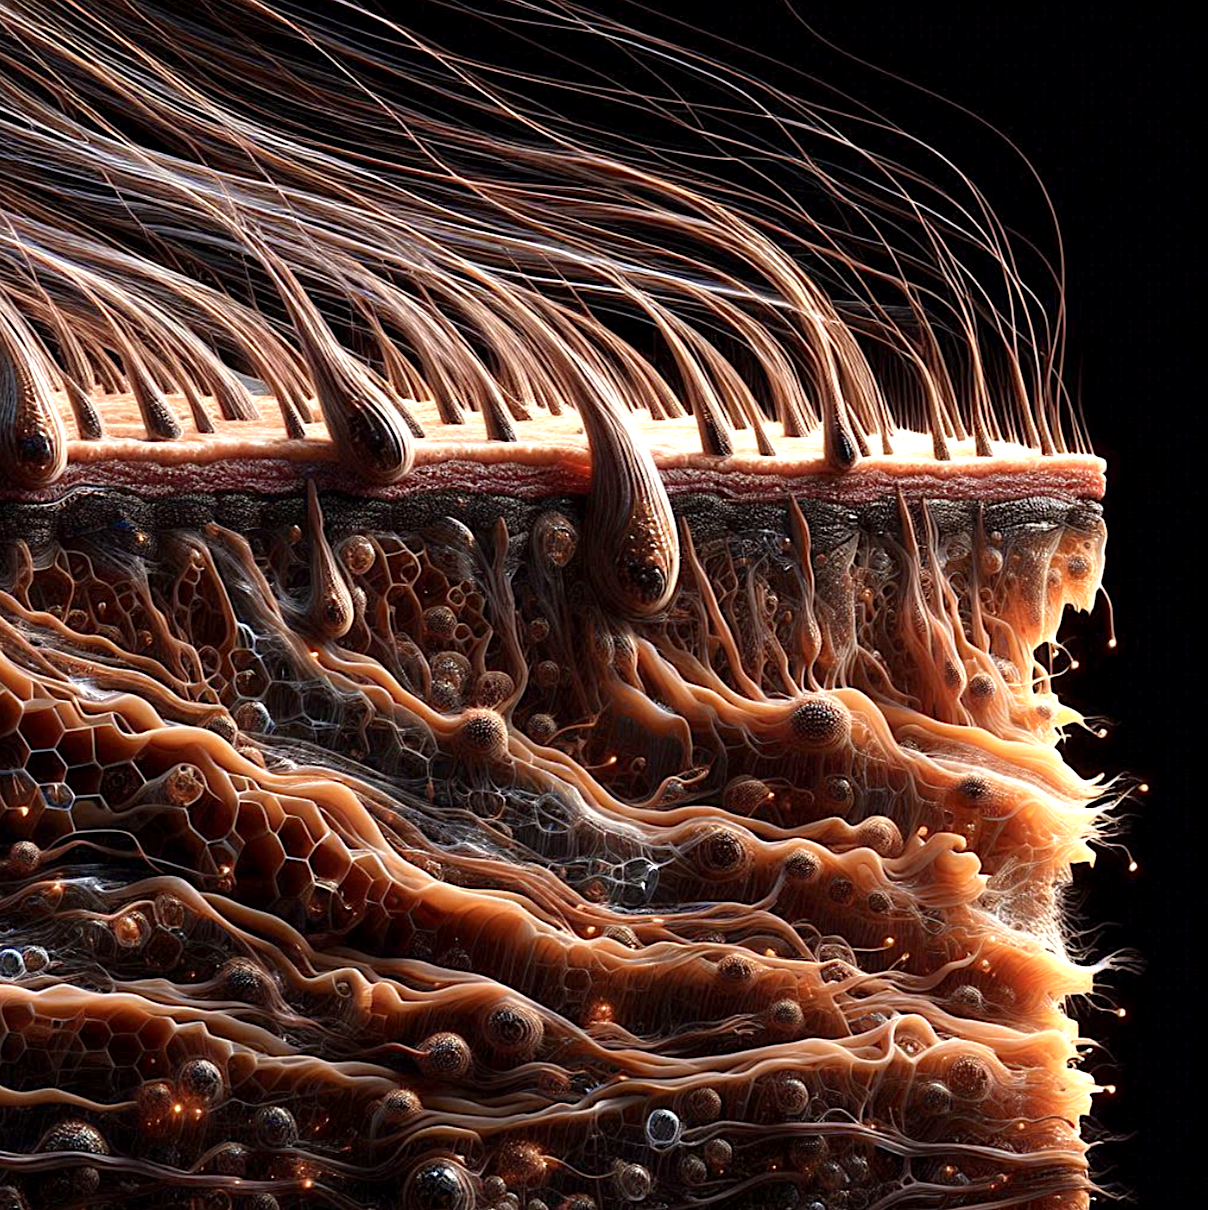
\includegraphics[width=0.7\linewidth]{Images/AI Skin 2025-06-11} 

}

\caption{AI Image of the Skin (Source: Microsoft Designer , Stunning Designs in a Flash, Image Generator, https://designer.microsoft.com/ 2025)}\label{fig:unnamed-chunk-8}
\end{figure}

Image created by Microsoft Designer\textsuperscript{5}.

\newpage

\subsection{The Structure of the Skin}\label{the-structure-of-the-skin}

The skin is composed of three primary layers: the \textbf{epidermis},
the \textbf{dermis}, and the \textbf{hypodermis} (also known as the
subcutaneous fat layer). Each layer performs specific functions
essential to maintaining homeostasis, immunity and overall health.

\subsubsection{The Epidermis}\label{the-epidermis}

The \textbf{epidermis} is the outermost layer of the skin and is
primarily composed of keratinocytes, which are specialised cells
responsible for the synthesis of keratin, cytokines, growth factors and
interleukins. This layer provides the first line of defence against
environmental pathogegns and is organised into four distinct strata,
arranged from superficial to deep.

\begin{itemize}
\tightlist
\item
  \emph{The Stratum corneum}
\item
  \emph{The Stratum granulosum}
\item
  \emph{The Stratum spinosum}
\item
  \emph{The Stratum basale} (also referred to as the \emph{stratum
  germinativum} or the basal cell layer).
\end{itemize}

An illustrative representation of the epidermis is provided
below\textsuperscript{6}.

\begin{figure}

{\centering 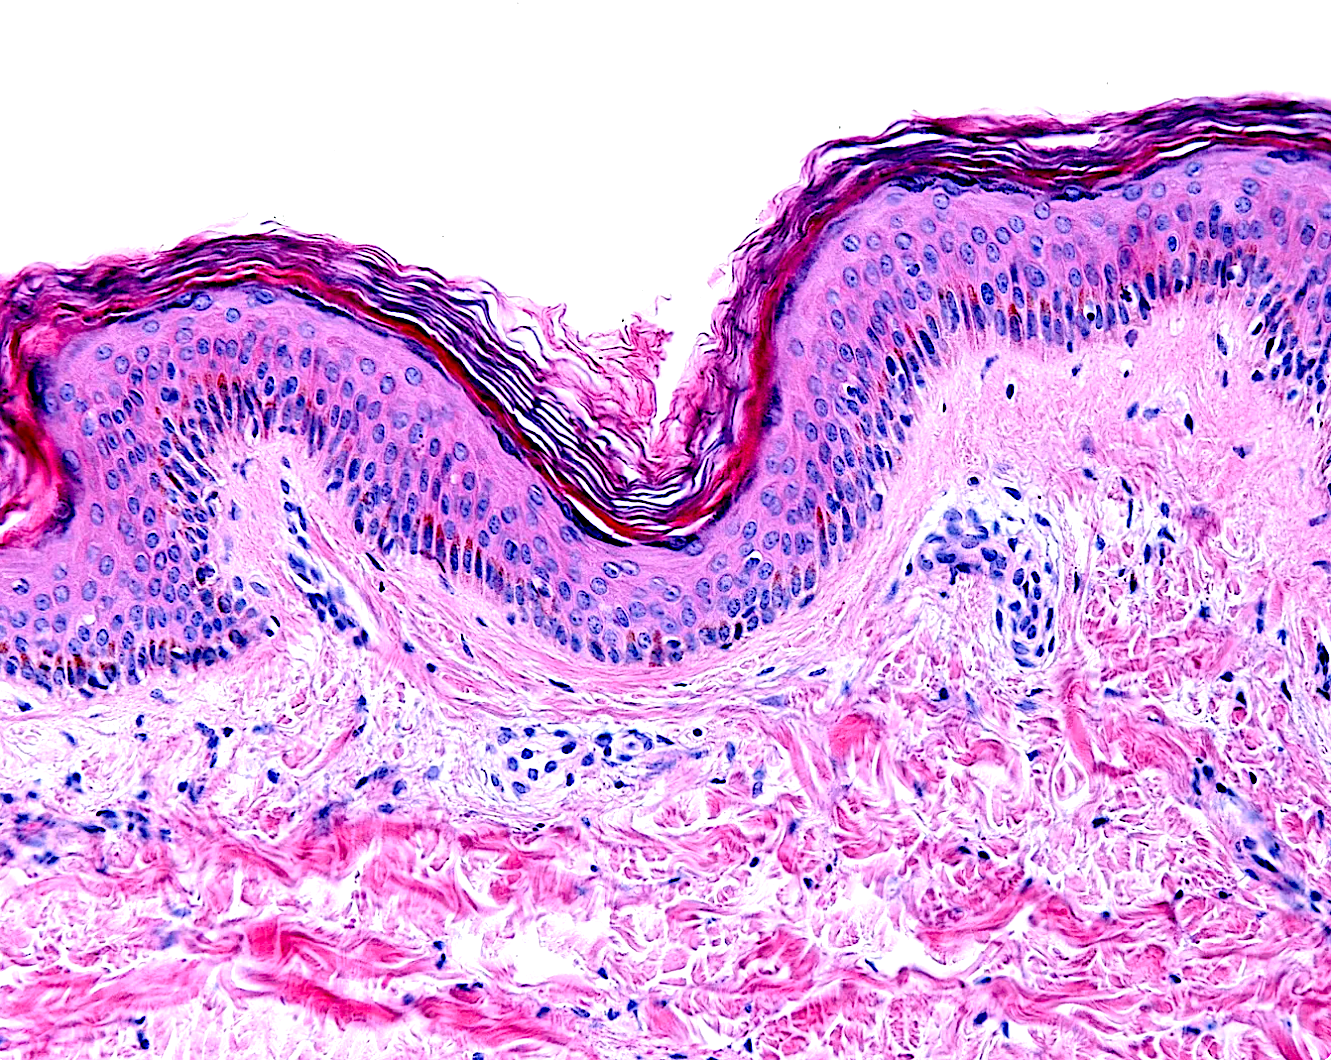
\includegraphics[width=0.9\linewidth]{Images/Epidermis} 

}

\caption{Structure of the epidermis with the different strata, resting on the dermis (Source: Shuttershock.com, Jose Luis Calvo, News Medical 2025)}\label{fig:unnamed-chunk-9}
\end{figure}

The \textbf{stratum corneum} consists of \emph{terminally
differentiated} keratinocytes. Terminally differentiated cells exit the
cell cycle as they can no longer divide. The keratinocytes become
corneocytes in the stratum corneum. \emph{Corneocytes} are non-viable,
enucleated cells\textsuperscript{7}.

The corneocytes function to minimise transepidermal water loss and
provide protection against mechanical and microbial damage. Keratin
produced in the underlying layers accumulates in the corneocytes, which
are eventually shed through a natural process known as desquamation.

The skin surface is interspersed with pores, which serve as conduits for
the excretion of sweat and sebum via eccrine and sebaceous glands,
respectively\textsuperscript{4}.

The \textbf{stratum spinosum}, or \emph{prickle cell layer}, lies above
the stratum basale and consists of keratinocytes connected by
desmosomes, which provide structural support. In this layer,
keratinocytes begin producing cytokeratins that form tonofibrils.
Langerhans cells, involved in immune defence, are also present in this
layer.

The \textbf{stratum granulosum} contains flattened keratinocytes that
undergo terminal differentiation. Keratinocytes accumulate keratohyalin
granules,involved in keratin aggregation, and lamellar bodies, which
secrete lipids that form a barrier to water loss. Keratinocytes in this
layer begin to lose their nuclei and organelles as they prepare for
transformation into dead corneocytes of the uppermost layer ;the stratum
corneum.

The \textbf{stratum basale} (or stratum germinativum) is the deepest
layer of the epidermis and plays a central role in skin regeneration.
This layer has mitotically active keratinocytes, which divide to
replenish the upper layers. In addition to keratinocytes, several other
specialised cells are found within this layer :

\begin{itemize}
\item
  \textbf{Melanocytes}, which produce melanin, the pigment responsible
  for skin colour and protection against ultraviolet (UV)
  radiation\textsuperscript{8}.
\item
  \textbf{Langerhans Cells}, (LCs) a type of dendritic cell (DC) that
  originate from hematopoietic stem cells in the bone marrow. They have
  a role in immune surveillance by recognising antigens and initiating
  T-cell responses\textsuperscript{7}.
\item
  \textbf{Merkel cells}, which are mechanoreceptors involved in the
  sensation of touch.
\item
  \textbf{Dendritic cells}, which also play a defence role in the immune
  response as they differentiate into macrophages\textsuperscript{7}.
\end{itemize}

Within the \textbf{stratum basale} UV radiation stimulates the
conversion of provitamin \(D_{3}\) into pre-vitamin \(D_{3}\) that
initiates the cutaneous synthesis of vitamin D. Subsequent hydroxylation
in the liver and kidneys leads to the production of the active form of
vitamin D\textsuperscript{7}.

The epidermis is not only a structural barrier but also a site of
pathological relevance. Several dermatological and systemic conditions
occur in this layer including \textbf{seborrhoeic dermatitis}
(dandruff), \textbf{psoriasis}, \textbf{atopic dermatitis} (eczema),
melanoma, \textbf{acne vulgaris }, \textbf{actinic keratosis} and
pressure ulcers (decubitus ulcers)\textsuperscript{4}.

\newpage

\subsubsection{The Dermis}\label{the-dermis}

The dermis is the middle layer of the skin, situated beneath the
epidermis, and serves as the primary site of structural and functional
support. It contains many essential components including blood vessels
such as capillaries\textsuperscript{7}, lymphatic vessels, sweat glands
, sebaceous glands, hair follicles, nerve endings, and specialised
sensory receptors. The dermis is primarily composed of \textbf{collagen}
and \textbf{elastin}, two fibrous proteins that confer tensile strength
and elasticity, respectively.

The dermis is subdivided into two distinct layers:

\begin{itemize}
\item
  \textbf{The papillary dermis}, the superficial layer, which is
  composed of loose connective tissue and contains capillaries and
  sensory neurons.
\item
  \textbf{The reticular dermis}, the deeper layer, composed of dense
  irregular connective tissue rich in collagen and elastin fibres,
  glands, hair follicles, and larger blood vessels.
\end{itemize}

The dermis contains sweat glands, sebaceous glands, blood vessels,
lymphatic vessels, and other structures critical to skin function. These
glands play essential roles in thermoregulation, lubrication, and
excretion. The eccrine glands are responsible for sweat production,
while the sebaceous glands secrete sebum to maintain skin hydration and
barrier function. Both are embedded within the dermal layer and are
regulated by hormonal and neural signals.

The dermis contains sweat glands, sebaceous glands, blood vessels,
lymphatic vessels, and other structures critical to skin function. These
glands play essential roles in thermoregulation, lubrication, and
excretion. The eccrine glands are responsible for sweat production,
while the sebaceous glands secrete sebum to maintain skin hydration and
barrier function. Both are embedded within the dermal layer and are
regulated by hormonal and neural signals.

Fibroblasts, the predominant cell type in the dermis, are responsible
for synthesising collagen proteins, and other components of the
extracellular matrix, which maintains the structural framework of
connective tissues. In addition to their structural role, fibroblasts
are actively involved in \textbf{wound healing} through production of
signalling molecules and matrix proteins\textsuperscript{9}.

Collagen is the most abundant protein in the human body and is found not
only in the skin but also in muscles, bones, tendons, ligaments, blood
vessels, internal organs and the gastrointestinal
lining\textsuperscript{10}. The primary amino acids in collagen include
glycine, proline and hydroxyproline, which assemble into a
characteristic triple-helix structure to form collagen fibrils. The
biosynthesis of this structure requires several cofactors, including
\textbf{vitamin C}, \textbf{zinc}, \textbf{copper} and
\textbf{manganese}\textsuperscript{10}.

Among the specialised mechanoreceptors in the dermis are Meissner's
corpuscles and Pacinian corpuscles, which detect mechanical stimuli such
as touch, pressure, and vibration. These corpuscles are multicellular
structures (of multiple cell types) consisting of a sensory nerve ending
surrounded by specialised Schwann cells.

The vascular network within the dermis plays a crucial role in
thermoregulation by adjusting blood flow in response to temperature
changes\textsuperscript{7}. The nerve endings transmit sensory
information such as touch, pain, and temperature\textsuperscript{7}.
Dermal Immune cells contribute to the inflammatory response following
injury or infection.

The dermis contains a diverse population of cells, including
fibroblasts, immune dendritic cells, macrophages, T lymphocytes, mast
cells, innate lymphoid cells, neutrophils, eosinophils, and natural
killer cells, neuronal cells and endothelial cells\textsuperscript{11}.

Among the immune cells, T lymphocytes are predominantly located in close
proximity to blood vessels, vessels, hair follicles and sweat glands
within the dermis. Subsets of T cells perform distinct immunological
functions: \textbf{Th1 cells } secrete cytokines that enhance the
capacity of other immune cells to target and eliminate pathogens l
however, dysregulation of Th1 activity may contribute to the development
of autoimmune disorders\textsuperscript{11}. \textbf{Th2 cells} are
primarily involved in the mediation of allergic responses. \textbf{Th17
cells} play a crucial role in defending against bacterial and fungal
infections and are implicated in the pathogenesis of inflammatory skin
diseases such as eczema and psoriasis.

In contrast, \textbf{regulatory T cells (Tregs)} modulate immune
responses by suppressing excessive inflammation through the release of
inhibitory signals and by eliminating over-active immune cells, thereby
maintaining immune homeostasis with the dermis\textsuperscript{11} .

Several conditions originate within the dermis, including wrinkles (due
to collagen degradation), cellulitis (a bacterial skin infection),
dermoid cysts (which may contain hair or teeth), sebaceous cysts, and
dermatofibromas.

An illustrative representation of the dermis containing sweat glands,
sebaceous glands, blood vessels, lymphatic vessels is shown
below\textsuperscript{12}.

\begin{figure}

\hfill{}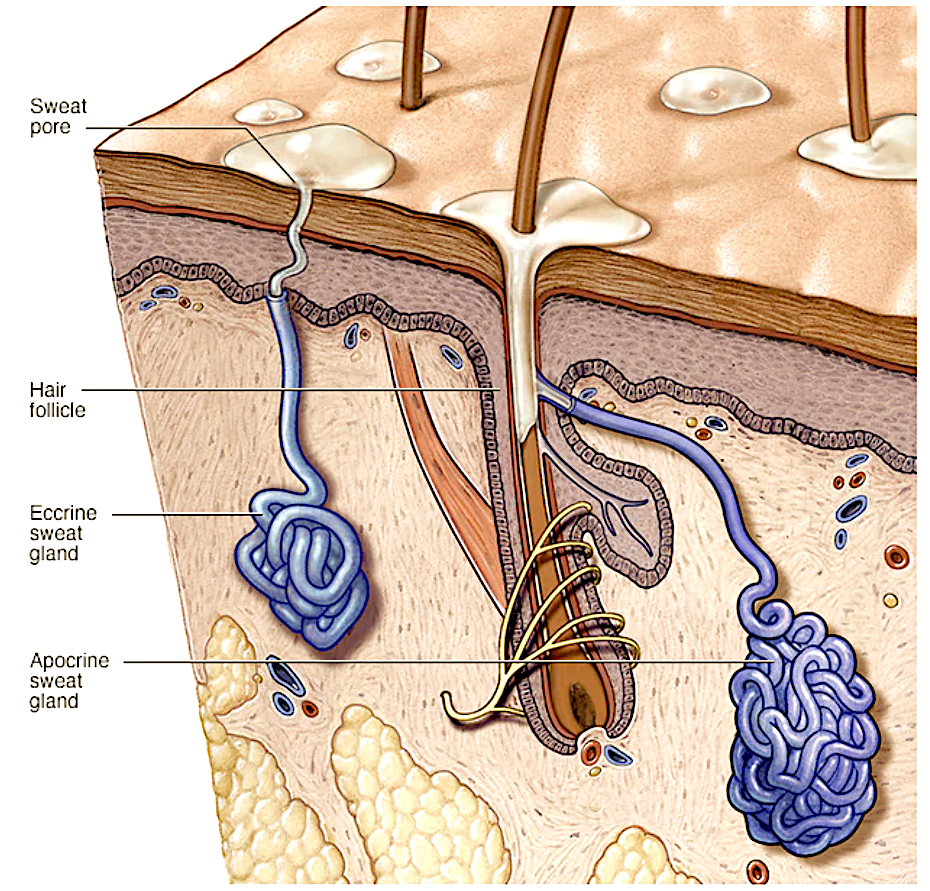
\includegraphics[width=0.8\linewidth]{Images/Glands} 

\caption{Eccrine \& sebaceous glands in the dermis (Source: Mayo Foundation, 2025)}\label{fig:unnamed-chunk-10}
\end{figure}

\subsubsection{The Hypodermis}\label{the-hypodermis}

The \textbf{hypodermis}, also known as the subcutaneous layer of fat,
lies beneath the dermis and primarily consists of adipose tissue. This
layer is composed of lipocytes that function to insulate the body,
maintain thermoregulation, and serve as an energy reserve. The
hypodermis also plays a crucial role in absorbing mechanical shock and
protecting underlying muscles and organs.

Structurally, the hypodermis includes the following key components:

\begin{itemize}
\item
  Fibroblasts: Cells responsible for the production of
  collagen\textsuperscript{13}. They also regulate the immune response
  to producing cytokines and chemokines\textsuperscript{11}.
\item
  Adipose tissue: Specialised are fatty tissues composed of
  lipocytes\textsuperscript{13}
\item
  Connective tissue: A network of collagen and elastin fibres that
  support and anchors, and gives structure to other
  tissues\textsuperscript{13}.
\item
  Blood vessels: Including arteries, veins and capillaries that supply
  the skin with oxygen rich blood and nutrients, while facilitating
  thermoregulation\textsuperscript{13}.
\item
  Lymphatic vessels: Structures involved in maintaining fluid
  homeostasis and transporting lymph, a fluid containing immune cells
  and waste products\textsuperscript{13}.
\item
  Hair follicles: Structures that anchor individual hair shafts and are
  associated with sebaceous glands and nerve endings.
\item
  Nerve fibres: Sensory neurons the body's sense of position and
  movement in space.
\end{itemize}

The hypodermis functions as a supportive and protective layer and has
important vascular, immune and sensory roles.

\begin{center}\rule{0.5\linewidth}{0.5pt}\end{center}

\newpage

\section{Streptococcus pyogenes}\label{streptococcus-pyogenes}

\subsection{Streptococcus pyogenes:Taxonomy, Morphology \& Clinical
Relevance}\label{streptococcus-pyogenestaxonomy-morphology-clinical-relevance}

\emph{Streptococcus pyogenes} is a Gram-positive, anaerobic bacterium
commonly referred to as Group A Streptococcus(GAS)\textsuperscript{15}.

The Gram-positive nature is due to a thick peptidoglycan layer in its
cell wall, which retains the crystal violet stain.

Structurally, \emph{S.pyogenes} is characterised by its beta-hemolytic
activity, meaning it causes complete lysis of red blood cells on blood
agar plates. Morphologically, the cells are small, spherical, and
typically arranged in chains, a feature that distinguishes them from
other bacterial species\textsuperscript{15}.

Taxonomically, \emph{S.pyogenes} is classified as follows:

\begin{itemize}
\item
  \textbf{Domain}: \emph{Bacteria}
\item
  \textbf{Kingdom}: \emph{Bacillati}
\item
  \textbf{Phylum}: \emph{Bacillota}
\item
  \textbf{Class}: \emph{Bacilli}
\item
  \textbf{Order}: \emph{Lactobacillales}
\item
  \textbf{Family}: \emph{Streptococcaceae}
\item
  \textbf{Genus}: \emph{Streptococcus }
\item
  \textbf{Species}: \emph{S.pyogenes}\textsuperscript{15}
\end{itemize}

As a highly adaptable pathogen, \emph{S.pyogenes} is capable of causing
a wide range of clinical diseases, from mild superficial infections to
severe invasive conditions. Its chain-like cellular arrangement and
distinct beta-hemolytic properties are key identifiers in both clinical
and microbiological contexts.

\subsection{Infection of Human Skin}\label{infection-of-human-skin}

\emph{Streptococcus pyogenes} is a significant pathogen responsible for
a wide spectrum of clinical diseases. Prompt diagnosis and treatment of
\emph{S.pyogenes} infections are critical due to the organism's capacity
to cause both superficial and systemic illnesses.

Skin infections caused by \emph{S.pyogenes} range from localised
conditions such as impetigo to more severe and invasive diseases,
including necrotising fasciitis, a life-threatening infection of the
deep dermal and subcutaneous tissues\textsuperscript{15}.

In addition to skin infections, \emph{S.pyogenes} is known to cause
pharyngitis, pneumonia, scarlet fever, acute post-streptococcal
glomerulonephritis, and the autoimmune condition rheumatic fever. In
chronic cases,\emph{S.pyogenes} may also contribute to the development
of rheumatic heart disease.

\begin{figure}

{\centering 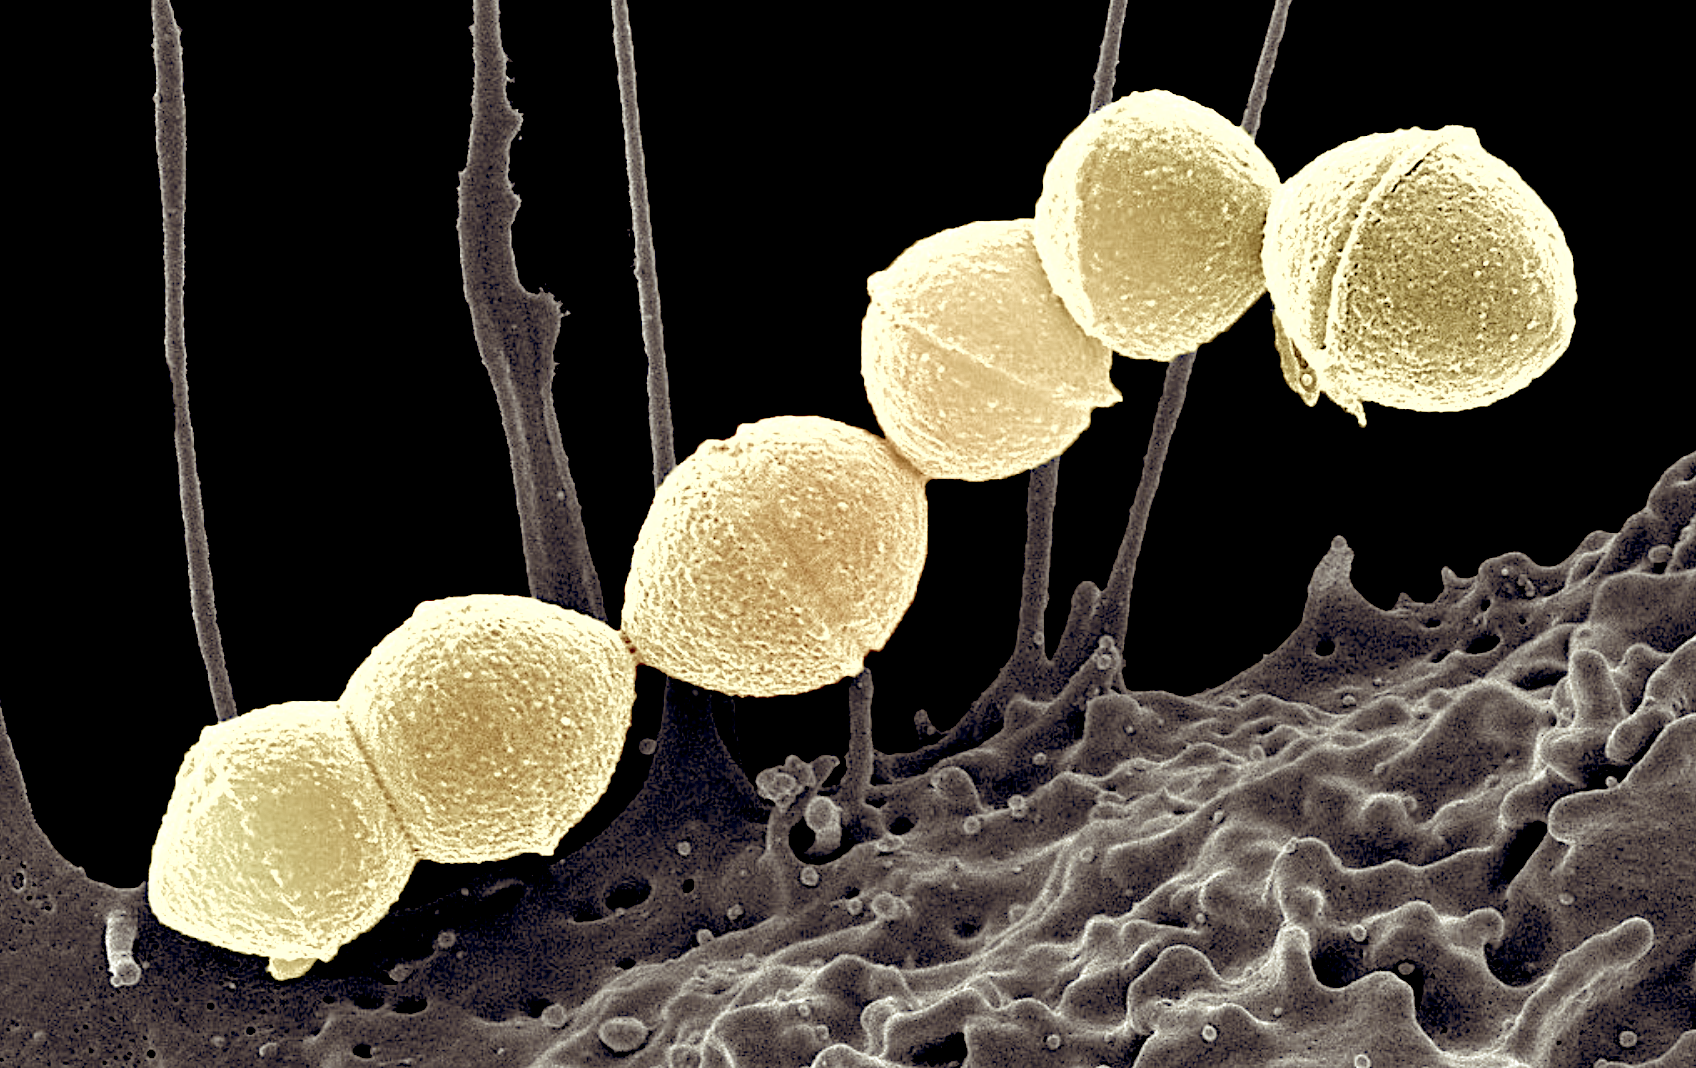
\includegraphics[width=0.9\linewidth]{Images/pyogenes2} 

}

\caption{Streptococcus pyogenes (Source:National Institute of Allergy and Infectious Diseases (NIAID), Flickr, December 29, 2022)}\label{fig:unnamed-chunk-11}
\end{figure}

\subsection{Virulence Factors of Streptococcus
pyogenes}\label{virulence-factors-of-streptococcus-pyogenes}

Virulence factors are molecules produced by pathogens that facilitate
infection, survival and damage within the host. \emph{S.pyogenes}
expresses a diverse array of virulence factors that enable its
pathogenicity, immune system invasion, and tissue
invasion\textsuperscript{15}.

\textbf{1. Capsules} The bacterium produces a capsule that protects it
from being engulfed by the host immune cells.

\textbf{2. Adherence Factors} Adherence factors (Adhesins), including
lipoteichoic acid (LTA) and fibronectin-binding proteins help the
bacterium to attach to host epithelial cells and tissues.

\textbf{3. Surface Proteins} Surface proteins such as M protein and
related members (e.g.~Mrp and Enn) play crucial roles in immune evasion.
These proteins have variable antigens which allow the pathogen to avoid
recognition by the host immune system.

\textbf{4. Enzymes} \emph{S.pyogenes} secretes several enzymes that
degrade host tissues and promote bacterial invasion. These include:

\begin{itemize}
\item
  \textbf{Streptokinase:} Converts plasminogen to plasmin, aiding in the
  breakdown of fibrin blood clots.
\item
  \textbf{Hyaluronidase:} Degrades hyaluronic acid in connective tissue,
  facilitating bacterial spread.
\item
  \textbf{DNases:} Break down extracellular DNA.
\end{itemize}

\textbf{5. Toxins} \emph{S.pyogenes} produces streptolysins (SLO and
SLS), exotoxins that lyse red blood cells and other host cells.
Additionally, streptococcal pyrogenic exotoxins (SPEs) are
super-antigens that activate T cells and induce a massive immune
response. At least three distinct SPEs have been
identified\textsuperscript{15}.

\subsubsection{The M Protein}\label{the-m-protein}

The M protein is a major virulence factor encoded by the emm gene
family, which is present in all \emph{S.pyogenes}
strains\textsuperscript{14}. These surface-anchored proteins are
involved in adherence, immune evasion, and resistance to phagocytosis.

The M protein is considered one of the most important virulence factors.

\begin{itemize}
\item
  \textbf{Structure:} The M protein is a coiled-coil molecule anchored
  in the bacterial membrane, with a highly variable N-terminal region
  responsible for antigenic diversity.
\item
  \textbf{Function:} It interferes with opsonisation and complement
  activation, making it a key player in immune system evasion. The
  M-protein changes surface antigens to make it harder for the host to
  recognise the pathogen.
\item
  \textbf{Variants:} M-related proteins such as Mrp and Enn, along with
  fibronectin-binding proteins, are also expressed and contribute to
  pathogenicity.
\end{itemize}

\subsubsection{F proteins}\label{f-proteins}

F proteins are another group of surface adhesins produced by
\emph{S.pyogenes}. These include fibrinogen-binding and
fibronectin-binding proteins, which facilitate tight adherence to host
tissues and are critical in the early stages of infection.

\subsubsection{Streptolysins and
Exotoxins}\label{streptolysins-and-exotoxins}

\begin{itemize}
\item
  Streptolysin O (SLO) and Streptolysin S (SLS) are cytolytic toxins
  that cause hemolysis and contribute to tissue damage during infection.
\item
  Streptococcal pyrogenic exotoxins (SPEs) are potent super-antigens
  activate T cells and stimulate a massive immune response, often
  leading to severe systemic symptoms.
\end{itemize}

\subsubsection{Lipoteichoic Acid and Vaccine
Targets}\label{lipoteichoic-acid-and-vaccine-targets}

Lipoteichoic acid is a key surface molecule involved in adherence and
immune activation, and it is under investigation as a potential target
for vaccine development\textsuperscript{15}.

\subsection{Antimicrobial Resistance}\label{antimicrobial-resistance}

\emph{S.pyogenes} also harbours genes associated with antimicrobial
resistance. Notable among these are:

\begin{itemize}
\tightlist
\item
  \textbf{lmrP:} Encodes a multidrug efflux pump
\item
  \textbf{tetM and tetL:} Confer resistance to tetracyclines.
\item
  \textbf{tgfT:} involved in resistance to specific antimicrobial
  agents\textsuperscript{17}.
\end{itemize}

These resistance genes highlight the need for continuous surveillance
and prudent use of antibiotics in treating \emph{S.pyogenes} infections.

\subsection{Biofilm Formation and Quorum Sensing in Streptococcus
pyogenes}\label{biofilm-formation-and-quorum-sensing-in-streptococcus-pyogenes}

Biofilms are structured microbial communities encased within a
self-produced extracellular matrix. In \emph{Streptococcus pyogenes},
biofilm formation facilitates communication between cells and
contributes to bacterial surviva, particularly under host immune
response and exposure to antibiotics. This communication is mediated by
a mechanism known as quorum sensing, which regulates gene expression in
response to cell density.

In \emph{S.pyogenes}, one of the key quorum sensing pathways involved in
biofilm development is the Rgg2/3 pathway.This pathway controls the
expression of genes involved in biofilm formation through the modulation
of short hydrophobic peptides, which act as quorum sensing pheromones,
also referred to as autoinducers.

Short hydrophobic peptides are initially synthesised in an immature form
within the bacterial cell. To become functionally active, these peptides
undergo a two-step processing mechanism. First, an intracellular
metalloprotease enzyme processes the SHPS. Subsequently, they undergo
further processing in the extracellular environment to reach their
mature, biologically active form.

The specific transport mechanism responsible for the SHP export and the
identity of the extracellular processing factor(s) remain to be
elucidated.

The Rgg2/3 pathway is essential for biofilm maturation and plays a
central role in \emph{S.pyogenes} pathogenesis, particularly in
facilitating persistent infections by enhancing resistance to host
immune defences and antimicrobial agents.

\newpage

\section{Melanoma}\label{melanoma}

\subsection{Introduction to Melanoma}\label{introduction-to-melanoma}

Melanoma is a highly prevalent form of skin cancer originating from the
melanocytes\textsuperscript{21}.

As mentioned in the earlier section, Melanocytes are cells that
contribute to skin colouration due to the creation of
melanin\textsuperscript{22}. A tumour occurs when the DNA mutates inside
of the Melanocyte cells\textsuperscript{23}. Melanoma is notable for its
high metastatic potential\textsuperscript{24}.

Melanoma has several distinct subtypes, including Acral
Melanoma\textsuperscript{25}, Mucosal Melanoma and Uveal Melanoma, each
arising in different anatomical sites and with unique molecular
profiles\textsuperscript{23}. In contrast to keratinocyte carcinomas
which include basal cell carcinoma and squamous cell carcinoma, these
melanomas originate from melanocytes\textsuperscript{25}.

\subsection{Related Skin Cancers}\label{related-skin-cancers}

Other rare cutaneous malignancies include Sebaceous Carcinoma and
Apocrine Adenocarcinoma, as well as Merkel Cell Carcinoma, a
neuroendocrine tumour strongly linked with exposure to ultraviolet
light. Although these cancers are less common than melanoma, they use
similar methods for diagnosis and molecular testing.

\begin{figure}

{\centering 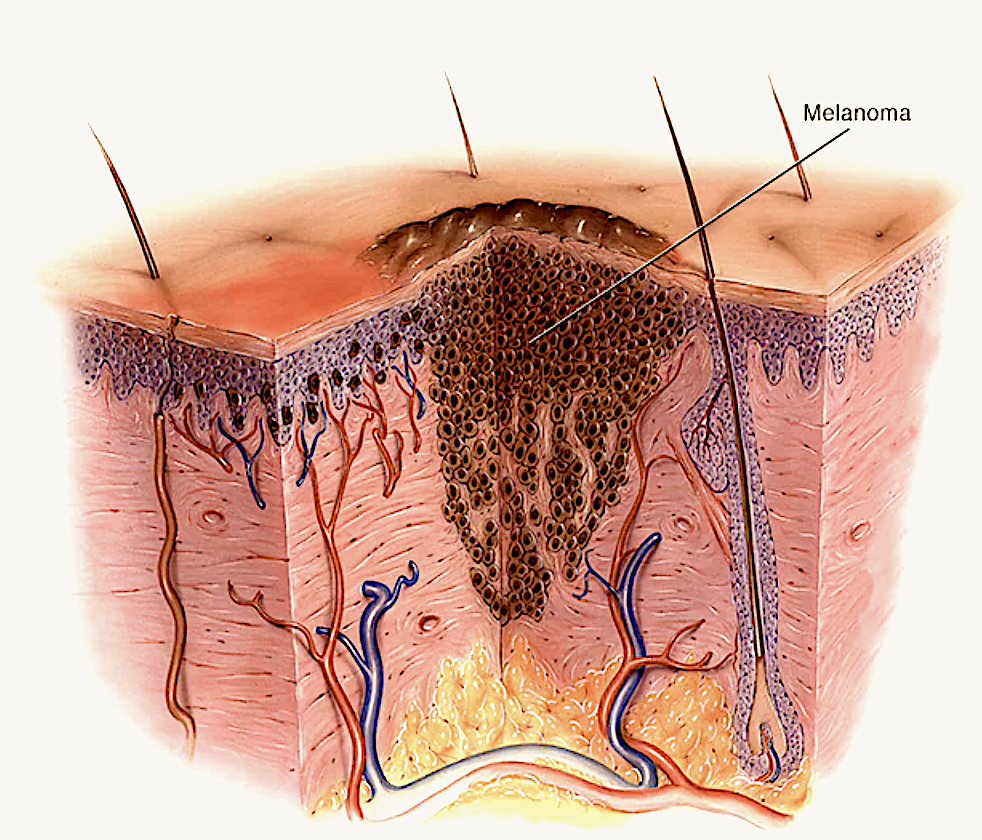
\includegraphics[width=0.9\linewidth]{Images/melanoma} 

}

\caption{Melanoma , Diseases and Conditons (Source Mayo Clinic, June 2025)}\label{fig:unnamed-chunk-12}
\end{figure}

\subsection{Melanocyte Development and Key
Pathways}\label{melanocyte-development-and-key-pathways}

The development of Melanocytes from neural crest cells (NCCs) is
regulated by a network of growth factors and intracellular signalling
pathways\textsuperscript{8}.

The most important regulatory molecules are endothelins and stem cell
factors. Stem cell factors are ligands for the c-Kit receptor. Other
critical growth factors include members of the Wnt protein family and
Neuregulin-1 (NRG1).

\subsubsection{Neuregulin-1}\label{neuregulin-1}

Neuregulin-1 (NRG1) is a growth factor that is known for its pleiotropic
effects\textsuperscript{18}. In addition to its role in melanocyte
biology, NRG1 is a key growth factor within the nervous system. It
promotes development of Schwann cells, glial cells that form the myselin
sheath, while also supporting neuron growth and enhancing synaptic
plasticity.

Furthermore, Neuregulin-1 contributes to the repair of the cardiac and
vascular tissues and acts via ErbB receptors.

\subsubsection{The Mitogen-Activated Protein Kinase (MAPK) signalling
pathway}\label{the-mitogen-activated-protein-kinase-mapk-signalling-pathway}

The Mitogen-Activated Protein Kinase (MAPK) signalling pathway is
central to the development of melanocytes\textsuperscript{21}. This
pathways plays a fundamental role in cell survival, proliferation and
differentiation. Signalling pathways are cascades of protein
interactions that respond to growth factors to direct the cells.

The MAPK pathway is activated when stem cell factors bind to the c-Kit
receptors on the melanoblast cell surface. The binding event initiates a
signalling cascade that leads to the activation of extracellular
signal-regulated kinases (ERKs). These kinases move to into the nucleus
and activate gene expression processes required for melanocyte
development and melanin biosynthesis.

Understanding how melanocytes normally develop is important for figuring
out how melanoma begins and spreads, since problems in these signalling
pathways are often involved in the disease process.

\subsection{Diagnosis and Imaging
Techniques}\label{diagnosis-and-imaging-techniques}

Magnetic Resonance Imaging (MRI) is the primary diagnostic tool for
Melanoma. MRI can be conducted with or without the use of contrast
agents to enhance lesion visualisation. In cases where imaging results
are inconclusive or suspicious, a biopsy is performed to obtain a tissue
sample for histological and molecular examination\textsuperscript{19}.

Histopathological analysis typically involves immunohistochemical
staining protocols, where tissue samples are incubated in biotin and
stained used haematoxylin blue/black nuclear stain and eosin pink
cytoplasmic stain to highlight cellular architecture and
pathology\textsuperscript{19}. To preserve biological integrity for
subsequent analyses, the specimen are often cryopreserved.

\subsection{Molecular and Genetic
Characterisation}\label{molecular-and-genetic-characterisation}

The identification of genetic mutations and molecular pathways involved
in melanoma is pivotal for both diagnosis and the development of
targeted therapies. Several genes are recognised as therapeutic
biomarkers and are investigated for the presence of
mutations\textsuperscript{19}.

Minimal Residual Disease (MRD) relates to the small number of cancer
cells that may remain in the body during or after treatment for Melanoma
and potentially lead to recurrence. Minimal Residual Disease is
typically assessed via liquid biopsy, a minimally invasive technique
that analyses circulating tumour DNA (ctDNA) in cerebrospinal fluid,
blood or urine.

This ctDNA analysis is referred to as fragmentomics and it uses advanced
techniques such as Digital PCR (dPCR) and Droplet Digital PCR (ddPCR) to
detect mutations.

Micro-RNAs (microRNA) also play a significant role in melanoma
pathogenesis. For example, miR-21 is often up-regulated in patients with
Melanoma and breast cancer. These non-coding RNAs are regulators of gene
expression and may serve as diagnostic and prognostic
biomarkers\textsuperscript{19}.

\subsection{Omics Approaches in Melanoma
Research}\label{omics-approaches-in-melanoma-research}

Comprehensive molecular profiling using omics based technologies has
changed the classification and understanding of
melanoma\textsuperscript{18}. Transcriptomics, which investigates the
full range of RNA transcripts expressed in tumour cells, provides
insight into the functional state of cancerous
tissues\textsuperscript{18}. Methylomics, focusing on DNA methylation
patterns reveals epigenetic modifications that contribute to the
oncogenesis and may serve as early diagnostic indicators. Microarray
based transcription profiling is employed for high throughput analysis
of gene expression, while cell surface proteomic analysis enables the
identification of differentially expressed membrane proteins.

\subsection{Molecular Subtyping and Future
Directions}\label{molecular-subtyping-and-future-directions}

Molecular subtyping of melanoma has become a cornerstone of personalised
oncology. By integrating data from genomics, transcriptomics and
proteomics, clinicians and researchers can classify tumours into
subtypes that inform prognosis and therapeutic response. This systems
biology approach not only enhances diagnostic precision but also opens
up avenues for novel targeted treatments\textsuperscript{26}.
Bioinformatics studies may provide a clearer understanding of the
molecular mechanisms behind melanoma metastasis\textsuperscript{26}.

Further insights into the overlap between cutaneous and Uveal Melanoma
have been gained through bioinformatics approaches which identify shared
gene expression signature and signalling pathways\textsuperscript{23}.
Such comparative analyses deepen the understanding of melanoma
heterogeneity and path the way for cross-subtype therapeutic
strategies\textsuperscript{26}.

\newpage

\section{Chapter III : RESEARCH
METHODS}\label{chapter-iii-research-methods}

\subsection{Overview of Research
Design}\label{overview-of-research-design}

This thesis investigates two biologically distinct but methodologically
complementary topics:

\begin{itemize}
\item
  The analysis of gene expression and immune-related pathways in
  melanoma
\item
  The genomic and structural analysis of virulence genes in
  Streptococcus pyogenes.
\end{itemize}

Despite being different biological systems, both studies rely on
bioinformatics and integrative genomic approaches.

\section{Topic I: Melanoma --- Gene Expression and Pathway
Analysis}\label{topic-i-melanoma-gene-expression-and-pathway-analysis}

\subsubsection{Topic 1: Melanoma Data and
Methods}\label{topic-1-melanoma-data-and-methods}

\subsubsection{Data Sources}\label{data-sources}

\begin{itemize}
\tightlist
\item
  National Centre for Biotechnology Information (NCBI) Gene Expression
  Omnibus (GEO) dataset
\end{itemize}

The data used in this study were obtained from publicly available
databases and include the \emph{Cutaneous Malignant Melanoma} dataset.
Specifically, I utilized gene expression data and associated clinical
information from tumour samples available through the National Centre
for Biotechnology Information (NCBI) Gene Expression Omnibus (GEO).

\begin{itemize}
\tightlist
\item
  Clinical information, GPL96 Affymetrix Microarray Data, gene
  expression
\end{itemize}

\begin{figure}

{\centering 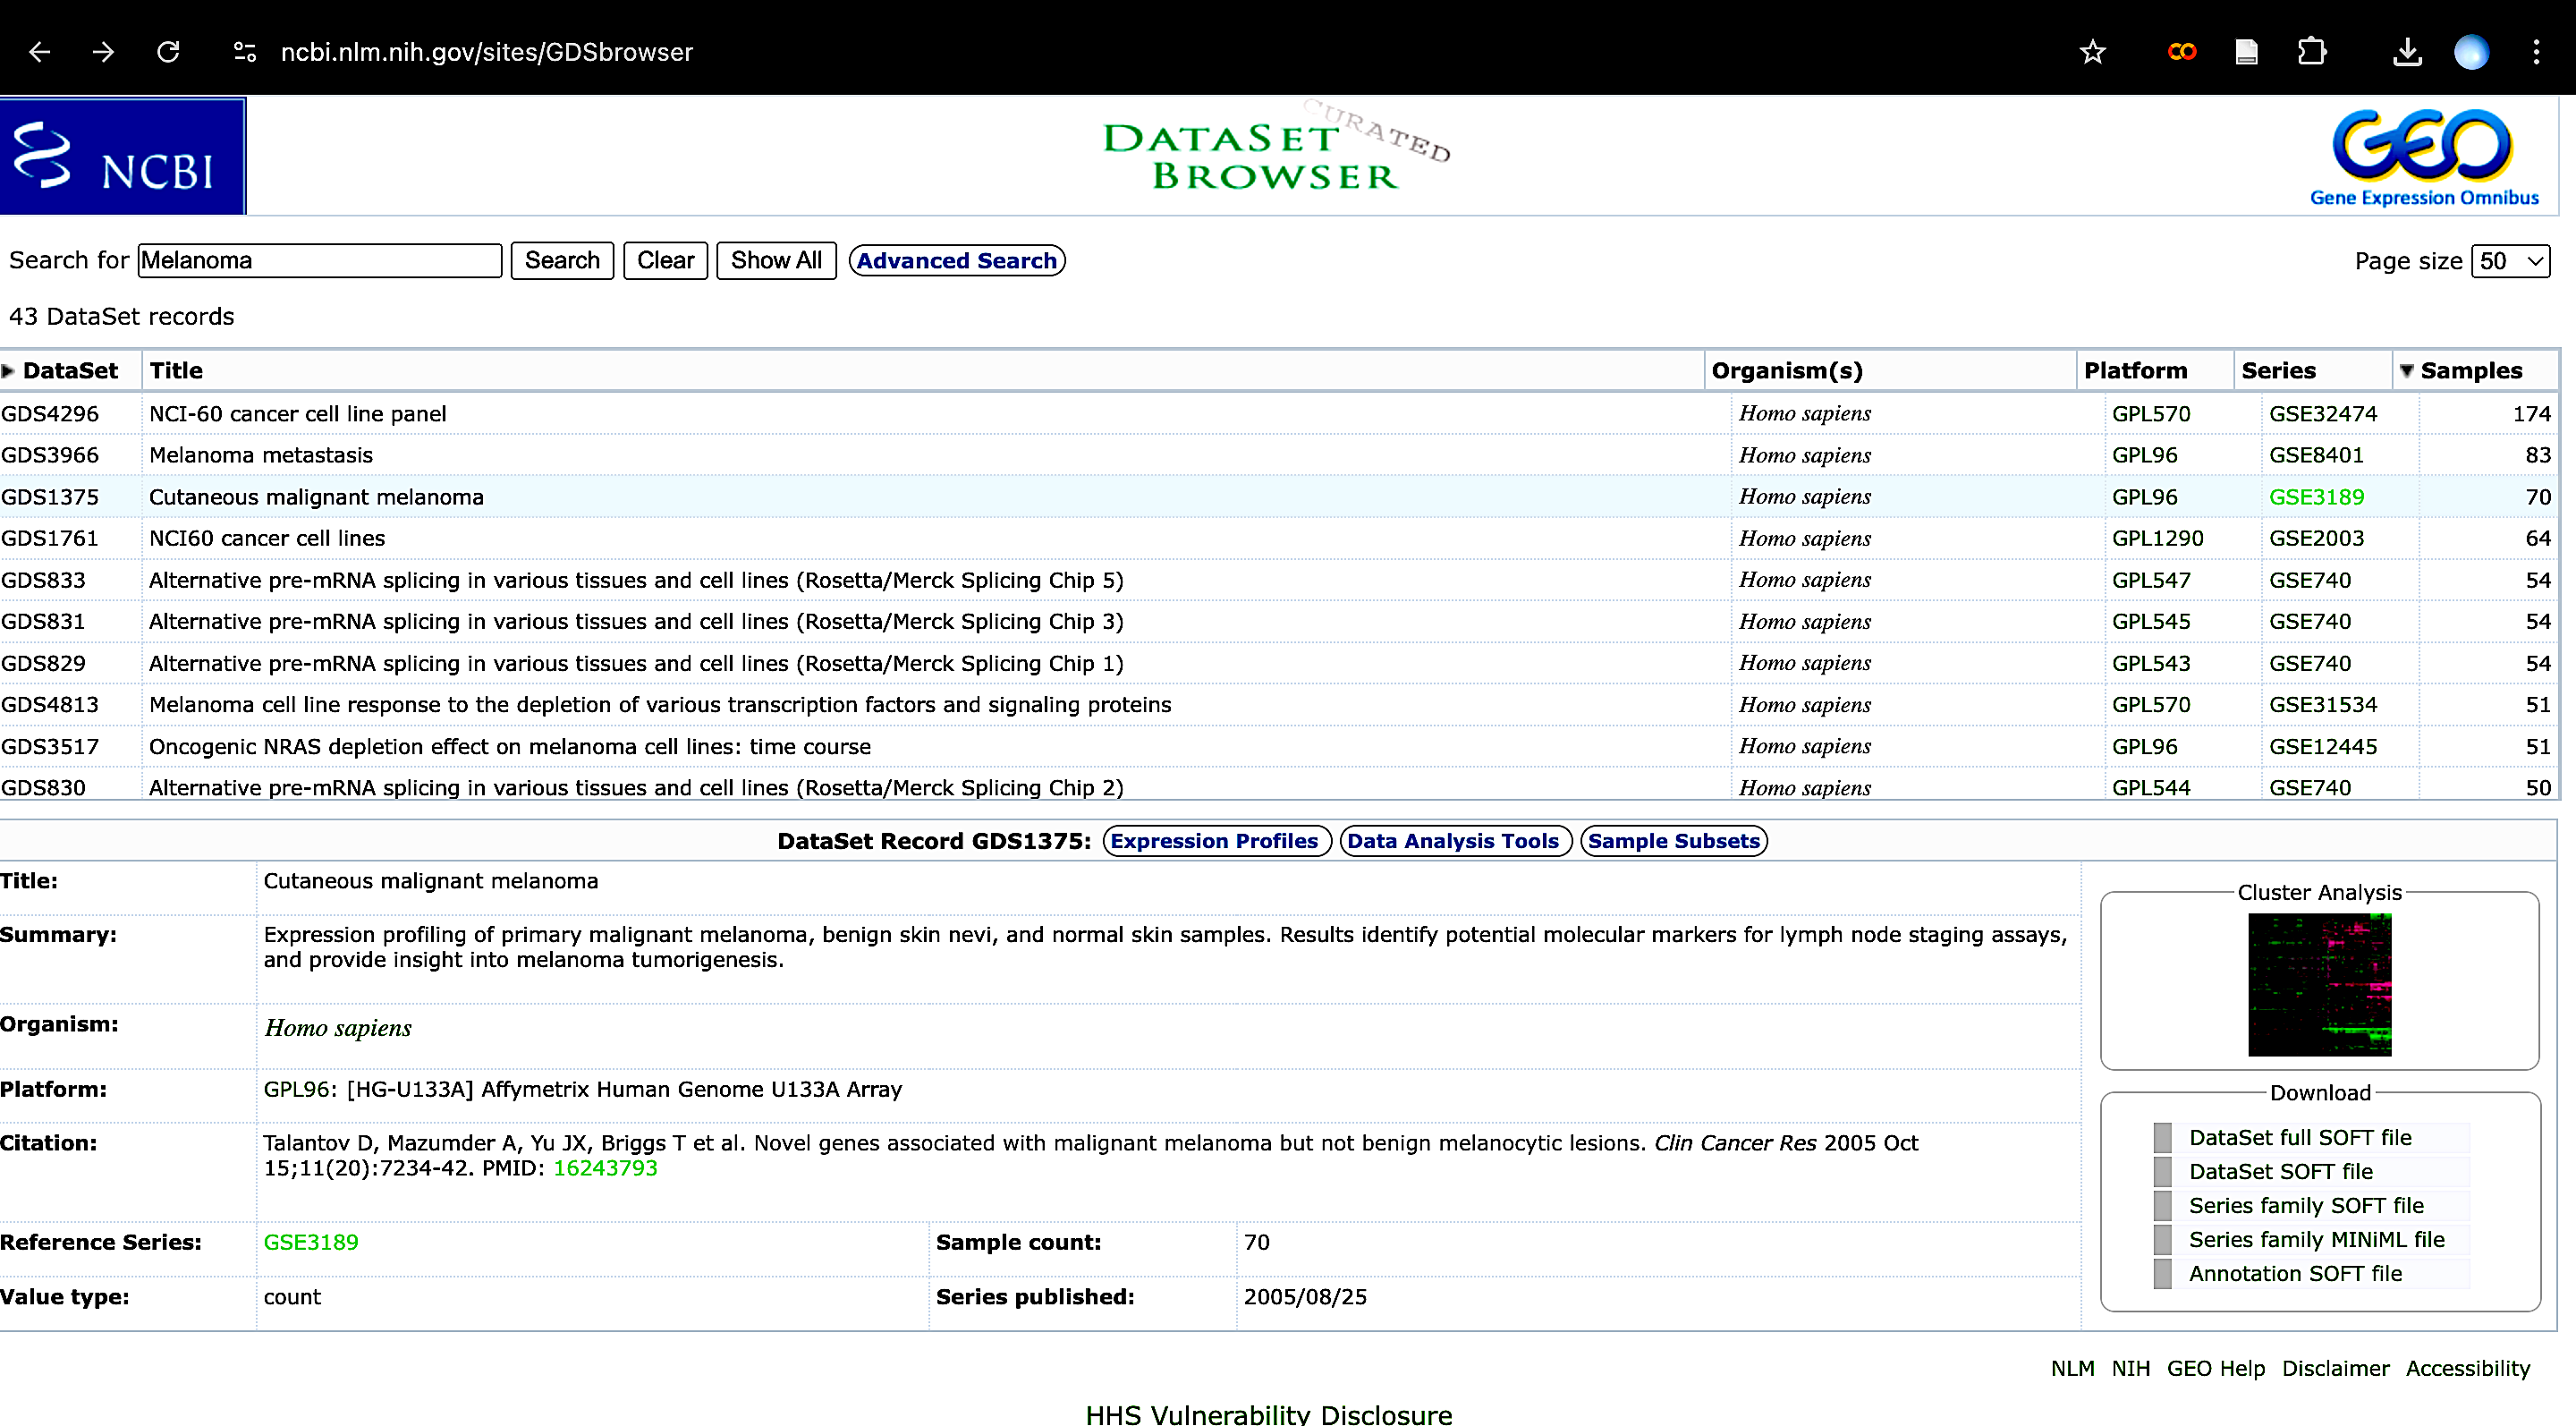
\includegraphics[width=0.9\linewidth]{Images/GEO_Data_2025-06-18 at 10.07.32} 

}

\caption{Cutaneous Malignant Melanoma dataset (Source:GDS Browser, 2025)}\label{fig:unnamed-chunk-14}
\end{figure}

\subsubsection{Data Preprocessing}\label{data-preprocessing}

Normalization, filtering, preprocessing tools

\subsubsection{Analytical Methods}\label{analytical-methods}

\begin{itemize}
\item
  Linear Models for Microarray and Omics Data (LIMMA) : Differential
  Gene Expression
\item
  Principal Component Analysis
\item
  KEGG/Pathway analysis
\item
  GSVA / ssGSEA
\item
  Tumour Analysis using the ESTIMATE package
\end{itemize}

\begin{center}\rule{0.5\linewidth}{0.5pt}\end{center}

\section{Topic II: Streptococcus pyogenes --- Virulence Gene \& Protein
Analysis}\label{topic-ii-streptococcus-pyogenes-virulence-gene-protein-analysis}

\subsubsection{Data Sources}\label{data-sources-1}

\begin{itemize}
\item
  Public databases (National Center for Biotechnology Information (NCBI)
  , AlphaFold)
\item
  Genomic Data Acquisition (FASTA files)
\item
  Download of genomic and protein sequence data of multiple S. pyogenes
  strains from NCBI.
\item
  Standardized file naming and merging into emm.fasta.
\item
  Include Table of emm genes and strains.
\end{itemize}

The genomic sequence data for this study was obtained from the National
Centre for Biotechnology Information (NCBI) GenBank database. The
complete coding sequences of several emm genes encoding the M protein
from \emph{Streptococcus pyogenes} of various strains were downloaded.
These DNA sequences were originally submitted to GenBank by Murayama et
al.~from the Laboratory of Molecular Cell Biology, School of Pharmacy,
Nihon University, Japan and subsequently published in the database.

These sequences represent a linear bacterial DNA fragment. Each fragment
contains the complete coding sequence for the M protein, a major
virulence factor of \emph{Streptococcus pyogenes}\textsuperscript{27}.

\subsubsection{Data Preparation}\label{data-preparation}

\begin{itemize}
\item
  Renaming FASTA files
\item
  Merging into emm.fasta (unix commands)
\end{itemize}

\subsubsection{Analytical Methods}\label{analytical-methods-1}

\begin{itemize}
\item
  MUSCLE alignment of emm genes
\item
  WebLogo Motif Analysis
\item
  Phylogenetic Tree Construction
\item
  Use aligned sequences to infer phylogeny and strain relationships.
\item
  Evaluate whether emm-type clusters correlate with virulence gene
  presence.
\item
  Protein Structure Prediction

  \begin{itemize}
  \tightlist
  \item
    Use Swiss-Model and PyMOL to model M protein structure
  \end{itemize}
\end{itemize}

\begin{center}\rule{0.5\linewidth}{0.5pt}\end{center}

\newpage

\section{Chapter IV: RESULTS AND
ANALYSIS}\label{chapter-iv-results-and-analysis}

\section{RESULTS - Topic I: Melanoma}\label{results---topic-i-melanoma}

\subsection{Overview of the Dataset}\label{overview-of-the-dataset}

The dataset selected for this study is the \emph{Cutaneous Malignant
Melanoma} dataset, identified by GEO Data Set (GDS) accession number
\textbf{GDS1375} and series number \textbf{GSE3189}, comprised of a
total of 70 samples. This dataset was made publicly available on the
25th day of August in 2005. It consists of microarray gene expression
profiles from three distinct sample groups: 45 malignant melanoma
samples, 18 benign skin nevus samples and 7 normal skin samples.

For the purposes of this analysis, the SOFT file was downloaded and both
the phenotype data and gene expression counts were extracted and
processed.From the full dataset, a subset was selected for differential
analysis, comprising of 21 malignant melanoma samples and 14 skin nevus
samples. The 7 normal skin samples were excluded from this comparative
analysis.

\begin{figure}

{\centering 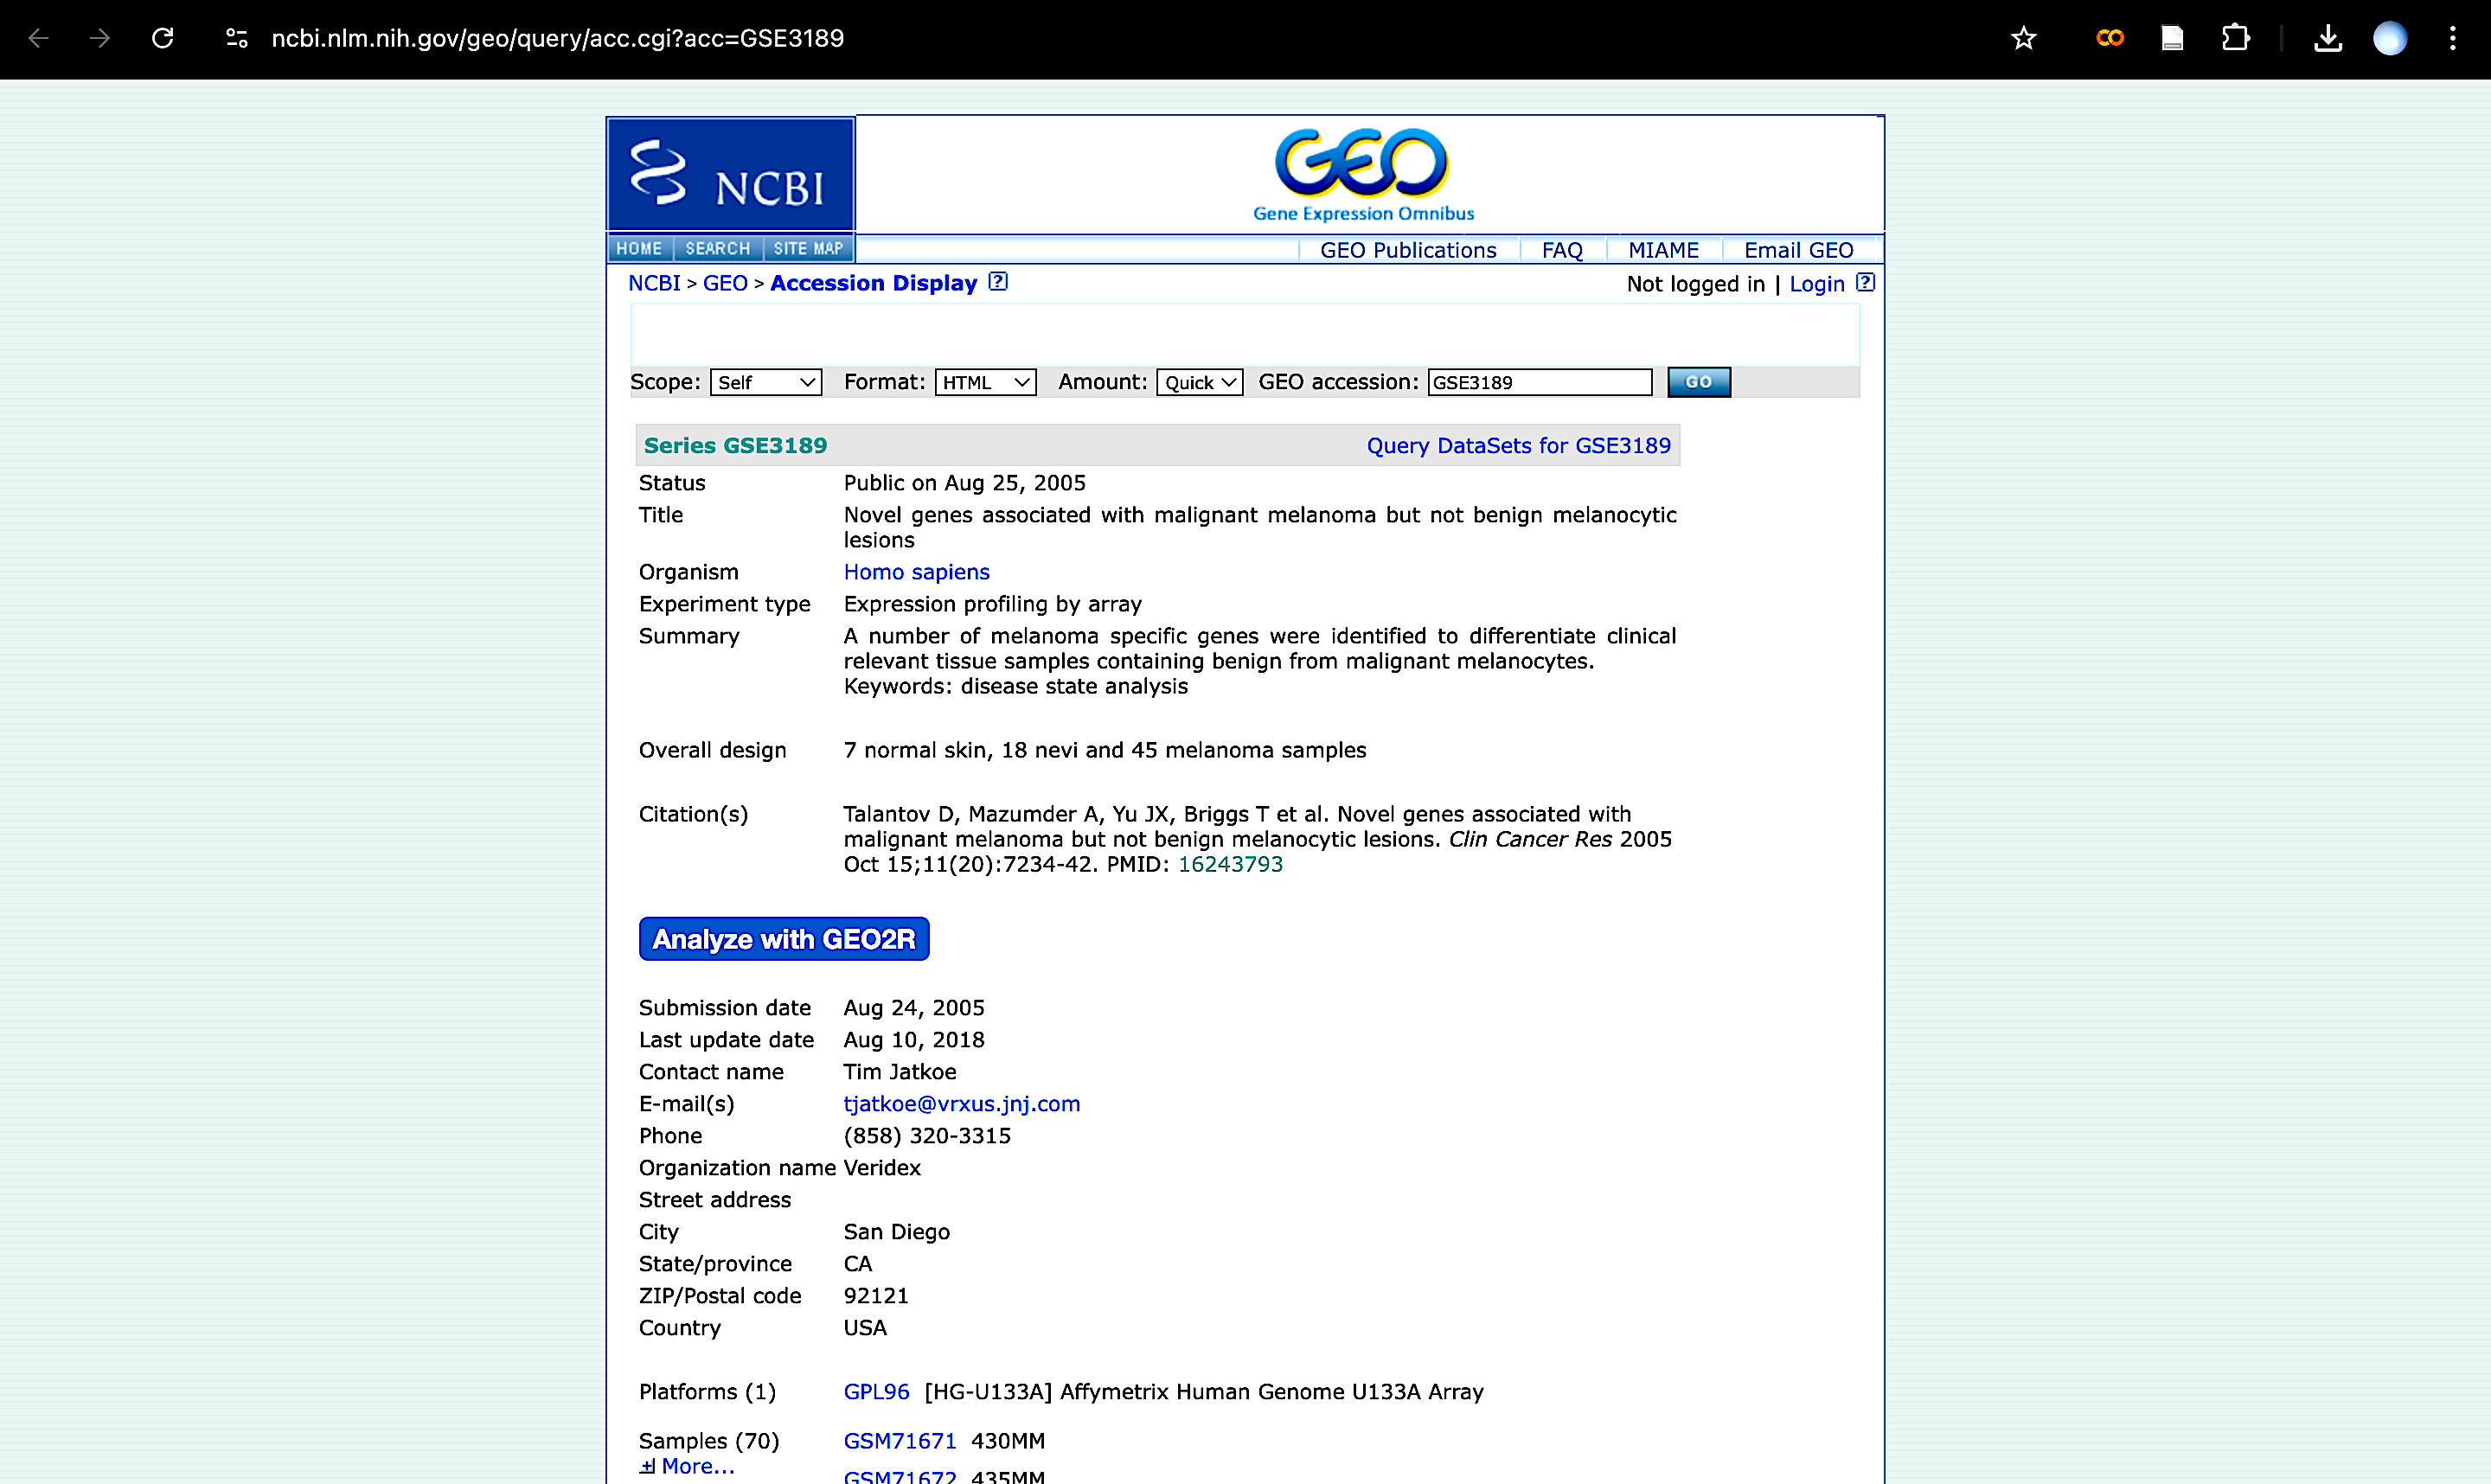
\includegraphics[width=0.9\linewidth]{Images/Gene_Expression_Omnibus2025-06-18 at 10.07.49} 

}

\caption{Selection of GSE3189 Series Data (Source:GDS Browser, 2025)}\label{fig:unnamed-chunk-15}
\end{figure}
\newpage

\newpage

\subsection{Differential Gene
Expression}\label{differential-gene-expression}

\subsubsection{Mean-variance trend}\label{mean-variance-trend}

\includegraphics{Thesis_Report_I_files/figure-latex/unnamed-chunk-21-1.pdf}

This is a diagnostic plot where each point represents a gene. The x-axis
shows the average log2-counts per million (logCPM) for each gene. The
y-axis shows the estimated variance (or square root of standard
deviation) of the log2 expression values for each gene. The trend line
is plotted over the points to estimate the mean-variance relationship in
the dataset. The mean-variance trend shows a relatively stable variance
across expression levels, indicating the normalization and statistical
modelling are appropriate for differential expression analysis.

\newpage

\begin{longtable}[]{@{}
  >{\raggedright\arraybackslash}p{(\columnwidth - 8\tabcolsep) * \real{0.4054}}
  >{\raggedright\arraybackslash}p{(\columnwidth - 8\tabcolsep) * \real{0.1081}}
  >{\raggedright\arraybackslash}p{(\columnwidth - 8\tabcolsep) * \real{0.1351}}
  >{\raggedright\arraybackslash}p{(\columnwidth - 8\tabcolsep) * \real{0.1757}}
  >{\raggedright\arraybackslash}p{(\columnwidth - 8\tabcolsep) * \real{0.1757}}@{}}
\caption{(Table of Top 20 Significantly Up-regulated
Genes)}\tabularnewline
\toprule\noalign{}
\begin{minipage}[b]{\linewidth}\raggedright
Gene Symbol
\end{minipage} & \begin{minipage}[b]{\linewidth}\raggedright
Log FC
\end{minipage} & \begin{minipage}[b]{\linewidth}\raggedright
Ave Expr
\end{minipage} & \begin{minipage}[b]{\linewidth}\raggedright
P-Value
\end{minipage} & \begin{minipage}[b]{\linewidth}\raggedright
Adj P-Value
\end{minipage} \\
\midrule\noalign{}
\endfirsthead
\toprule\noalign{}
\begin{minipage}[b]{\linewidth}\raggedright
Gene Symbol
\end{minipage} & \begin{minipage}[b]{\linewidth}\raggedright
Log FC
\end{minipage} & \begin{minipage}[b]{\linewidth}\raggedright
Ave Expr
\end{minipage} & \begin{minipage}[b]{\linewidth}\raggedright
P-Value
\end{minipage} & \begin{minipage}[b]{\linewidth}\raggedright
Adj P-Value
\end{minipage} \\
\midrule\noalign{}
\endhead
\bottomrule\noalign{}
\endlastfoot
NTRK3 & 5.574 & 5.693 & 0.0000129 & 0.0001071 \\
WFDC1 & 5.222 & 4.888 & 0.0000264 & 0.0001952 \\
HEY1 & 5.047 & 4.436 & 0.0000000 & 0.0000000 \\
GDF15 & 4.964 & 5.666 & 0.0000000 & 0.0000000 \\
NTRK3 & 4.946 & 5.498 & 0.0001644 & 0.0009026 \\
PHACTR1 & 4.654 & 4.232 & 0.0000001 & 0.0000024 \\
NTRK3 & 4.639 & 5.913 & 0.0000029 & 0.0000314 \\
SPP1 & 4.363 & 5.332 & 0.0000000 & 0.0000004 \\
ABHD2 & 4.228 & 4.999 & 0.0000002 & 0.0000035 \\
NTRK3 & 3.960 & 6.619 & 0.0000000 & 0.0000011 \\
KIF23 & 3.849 & 2.064 & 0.0001005 & 0.0005954 \\
MIR6872 /// SEMA3B & 3.819 & 3.665 & 0.0000005 & 0.0000077 \\
RNFT2 & 3.800 & 1.402 & 0.0000763 & 0.0004709 \\
NTRK3 & 3.792 & 6.718 & 0.0000001 & 0.0000016 \\
RASGRF1 & 3.698 & 1.962 & 0.0044561 & 0.0144427 \\
NTRK3 & 3.668 & 6.624 & 0.0000001 & 0.0000014 \\
UBE2S & 3.557 & 5.534 & 0.0000000 & 0.0000003 \\
ATP6V0E2 & 3.540 & 6.915 & 0.0000000 & 0.0000000 \\
BCL2A1 & 3.531 & 4.655 & 0.0000000 & 0.0000000 \\
ARHGAP8 /// PRR5-ARHGAP8 & 3.522 & 2.658 & 0.0147619 & 0.0385832 \\
\end{longtable}

\begin{longtable}[]{@{}
  >{\raggedright\arraybackslash}p{(\columnwidth - 8\tabcolsep) * \real{0.3731}}
  >{\raggedright\arraybackslash}p{(\columnwidth - 8\tabcolsep) * \real{0.1194}}
  >{\raggedright\arraybackslash}p{(\columnwidth - 8\tabcolsep) * \real{0.1493}}
  >{\raggedright\arraybackslash}p{(\columnwidth - 8\tabcolsep) * \real{0.1642}}
  >{\raggedright\arraybackslash}p{(\columnwidth - 8\tabcolsep) * \real{0.1940}}@{}}
\caption{(Table of Top 20 Significantly Down-regulated
Genes)}\tabularnewline
\toprule\noalign{}
\begin{minipage}[b]{\linewidth}\raggedright
Gene Symbol
\end{minipage} & \begin{minipage}[b]{\linewidth}\raggedright
Log FC
\end{minipage} & \begin{minipage}[b]{\linewidth}\raggedright
Ave Expr
\end{minipage} & \begin{minipage}[b]{\linewidth}\raggedright
P-Value
\end{minipage} & \begin{minipage}[b]{\linewidth}\raggedright
Adj P-Value
\end{minipage} \\
\midrule\noalign{}
\endfirsthead
\toprule\noalign{}
\begin{minipage}[b]{\linewidth}\raggedright
Gene Symbol
\end{minipage} & \begin{minipage}[b]{\linewidth}\raggedright
Log FC
\end{minipage} & \begin{minipage}[b]{\linewidth}\raggedright
Ave Expr
\end{minipage} & \begin{minipage}[b]{\linewidth}\raggedright
P-Value
\end{minipage} & \begin{minipage}[b]{\linewidth}\raggedright
Adj P-Value
\end{minipage} \\
\midrule\noalign{}
\endhead
\bottomrule\noalign{}
\endlastfoot
KRT15 & -8.013 & 3.912 & 0.0000000 & 0.0000000 \\
KRT14 & -7.298 & 6.514 & 0.0000000 & 0.0000000 \\
LOR & -6.931 & 5.048 & 0.0000000 & 0.0000000 \\
LGALS7 /// LGALS7B & -6.740 & 5.159 & 0.0000000 & 0.0000000 \\
KRT1 & -6.686 & 6.289 & 0.0000000 & 0.0000000 \\
SERPINB5 & -6.510 & 3.593 & 0.0000000 & 0.0000000 \\
PKP1 & -6.493 & 3.489 & 0.0000002 & 0.0000028 \\
KRT5 & -6.399 & 6.329 & 0.0000000 & 0.0000000 \\
LY6D & -6.246 & 3.688 & 0.0000000 & 0.0000000 \\
S100A7 & -6.224 & 4.062 & 0.0000008 & 0.0000109 \\
FGFR3 & -6.213 & 3.892 & 0.0000002 & 0.0000035 \\
HOPX & -6.075 & 4.480 & 0.0000000 & 0.0000000 \\
AQP3 & -5.998 & 5.094 & 0.0000000 & 0.0000000 \\
SFN & -5.965 & 3.973 & 0.0000000 & 0.0000010 \\
TACSTD2 & -5.873 & 5.161 & 0.0000000 & 0.0000000 \\
PPL & -5.805 & 3.711 & 0.0000000 & 0.0000000 \\
SPRR1A & -5.713 & 2.635 & 0.0031335 & 0.0107551 \\
CHL1 & -5.709 & 3.169 & 0.0000000 & 0.0000000 \\
DSP & -5.691 & 5.536 & 0.0000000 & 0.0000000 \\
FLG & -5.622 & 4.183 & 0.0000002 & 0.0000032 \\
\end{longtable}

\newpage

\subsubsection{Volcano Plot}\label{volcano-plot}

\begin{figure}

{\centering 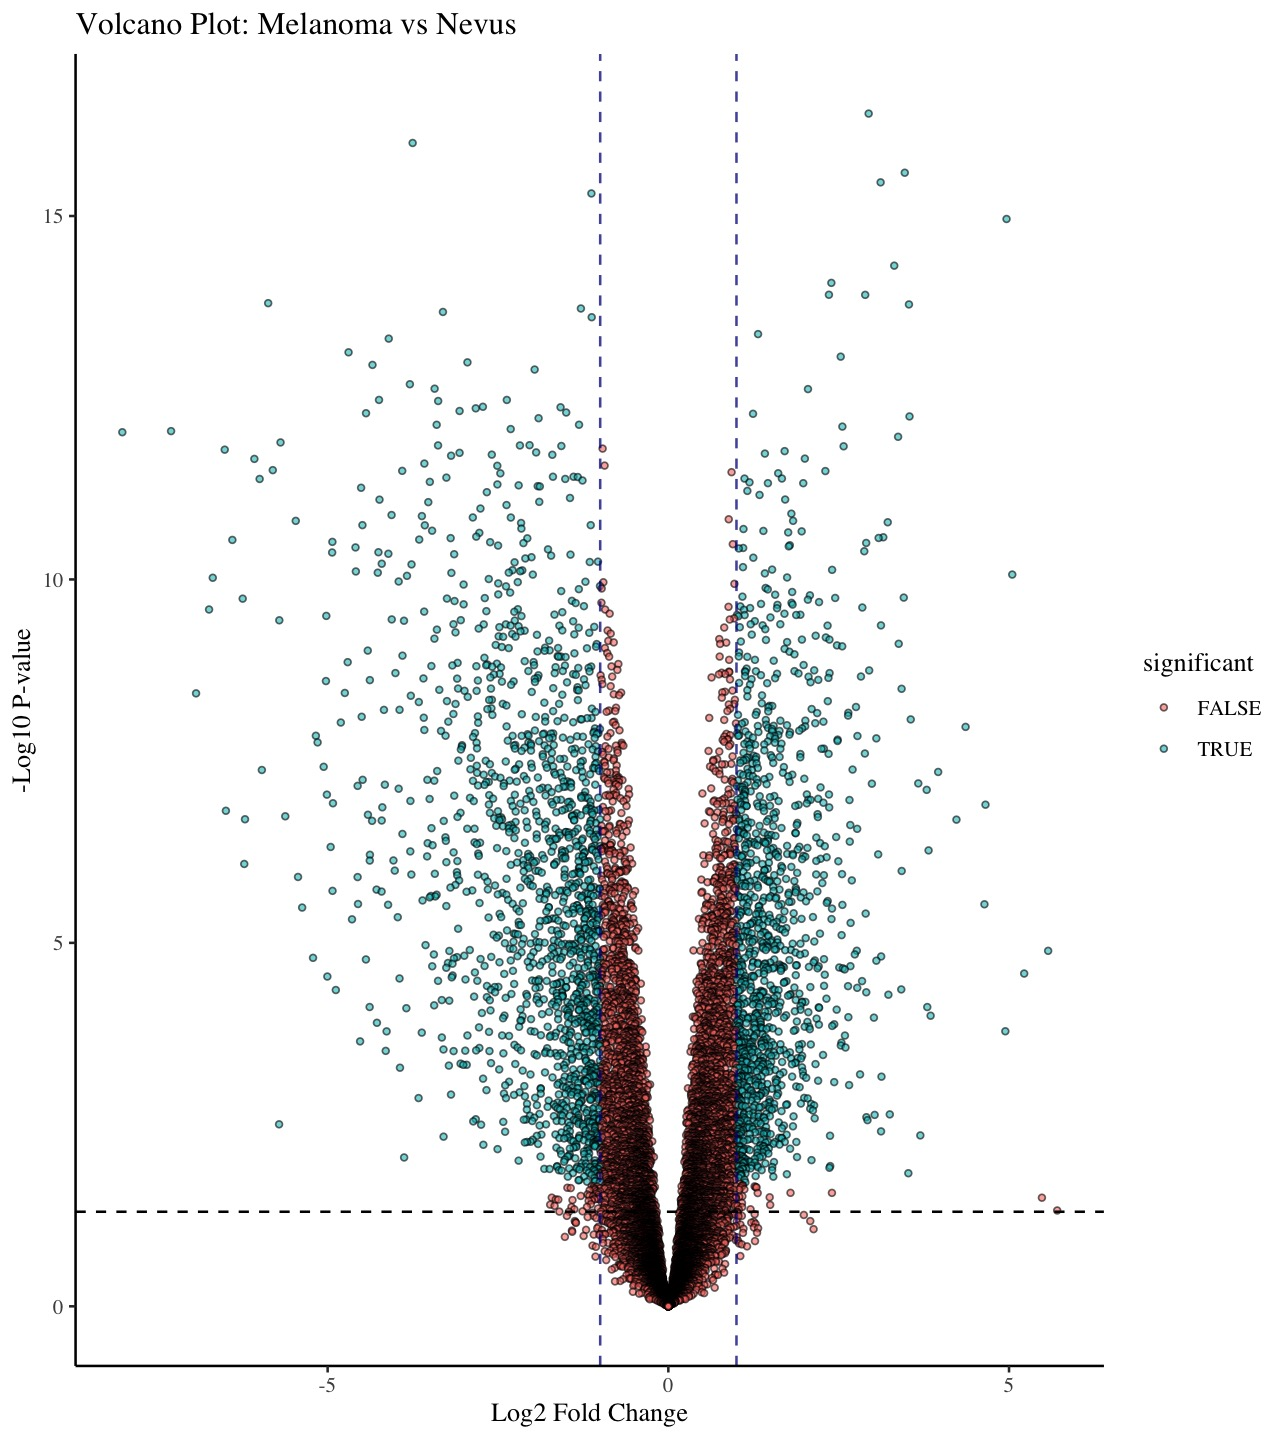
\includegraphics[width=0.8\linewidth]{Images/Volcano_Plot} 

}

\caption{Volcano Plot I }\label{fig:unnamed-chunk-23}
\end{figure}

\begin{figure}

{\centering 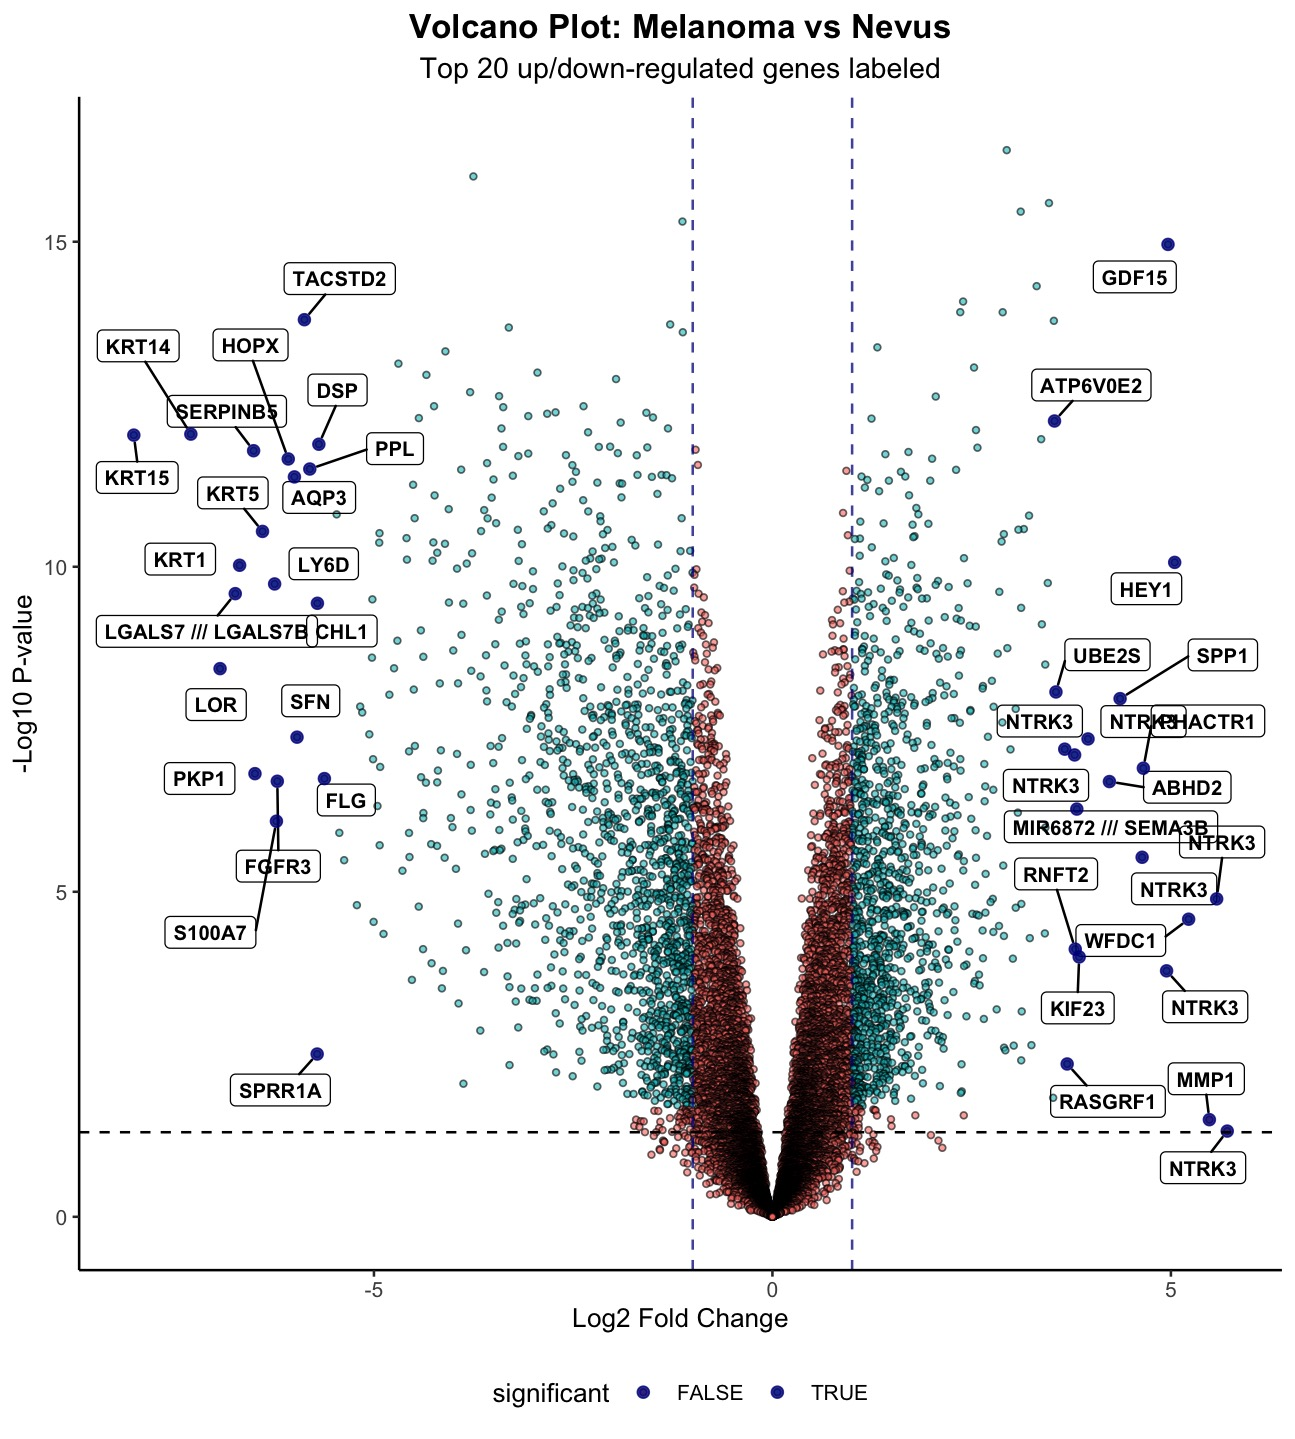
\includegraphics[width=0.8\linewidth]{Images/Volcano_Labelled} 

}

\caption{Volcano Plot II}\label{fig:unnamed-chunk-24}
\end{figure}

\newpage

\subsubsection{MA Plot}\label{ma-plot}

\begin{figure}

{\centering 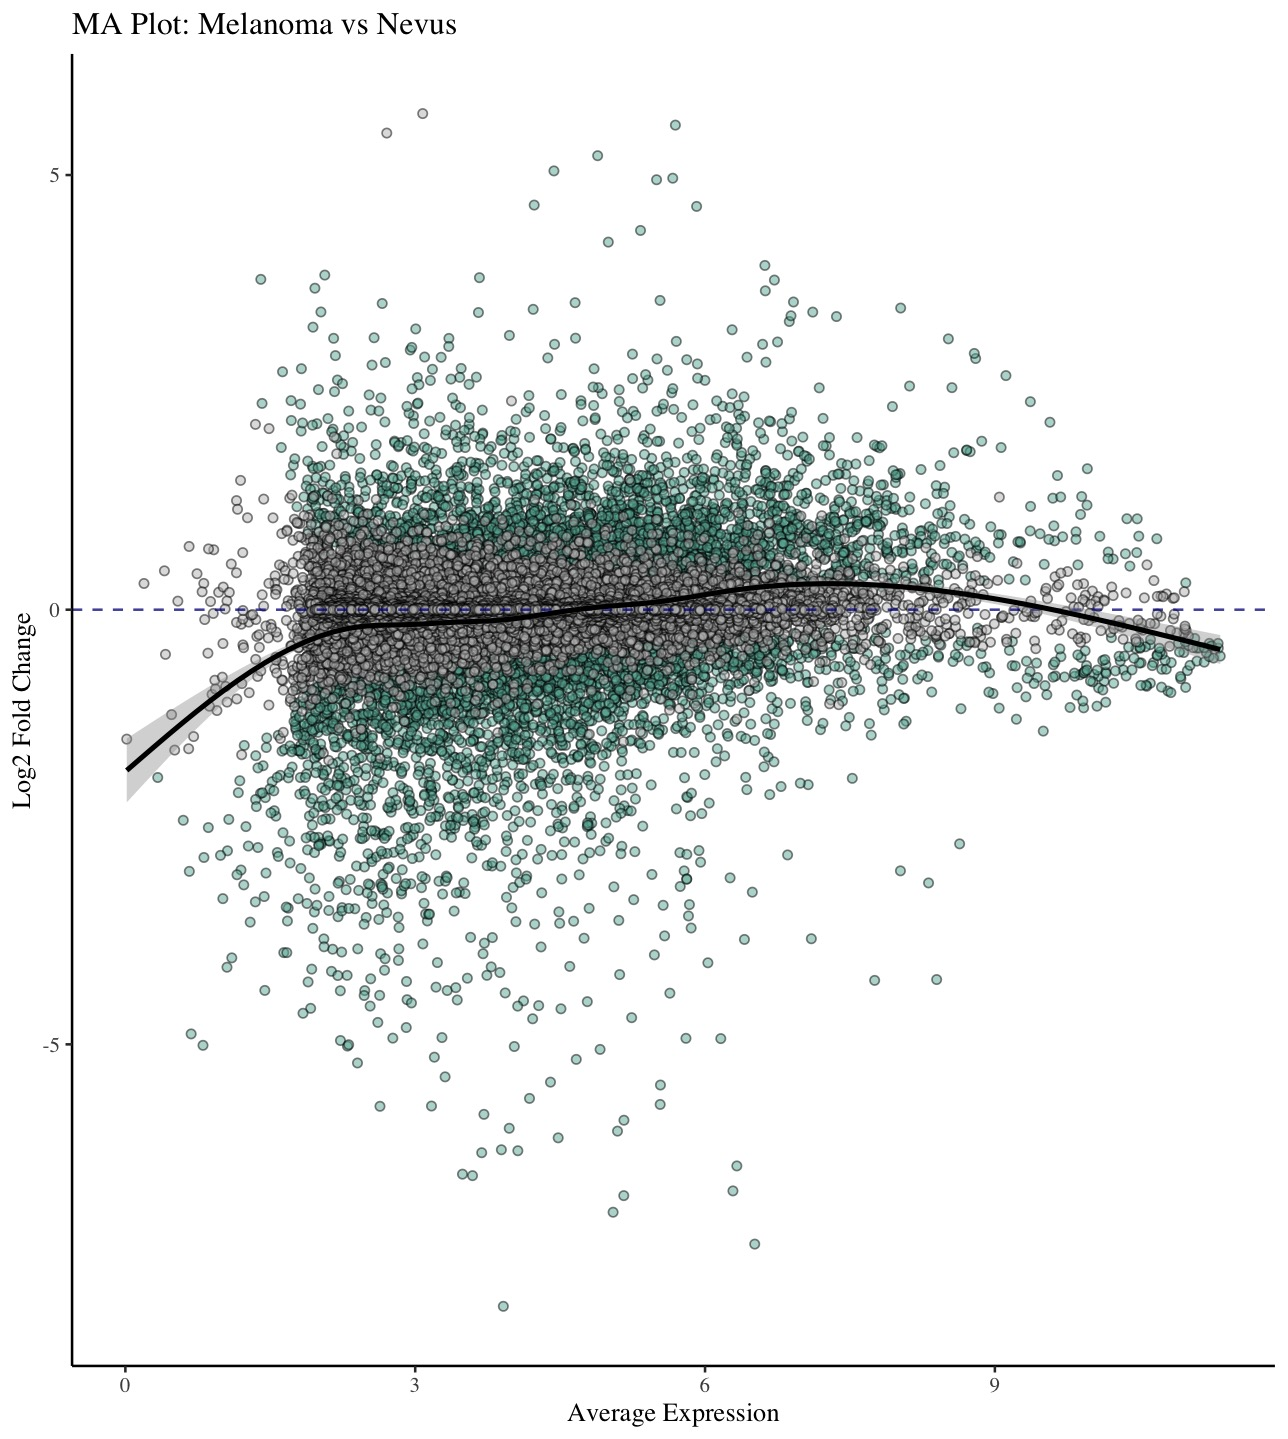
\includegraphics[width=0.8\linewidth]{Images/MA_Plot} 

}

\caption{MA Plot}\label{fig:unnamed-chunk-25}
\end{figure}

\newpage

\subsection{Principal Component Analysis (PCA) \&
Clustering}\label{principal-component-analysis-pca-clustering}

\subsubsection{Sample Correlation
Heatmap}\label{sample-correlation-heatmap}

\begin{figure}

{\centering 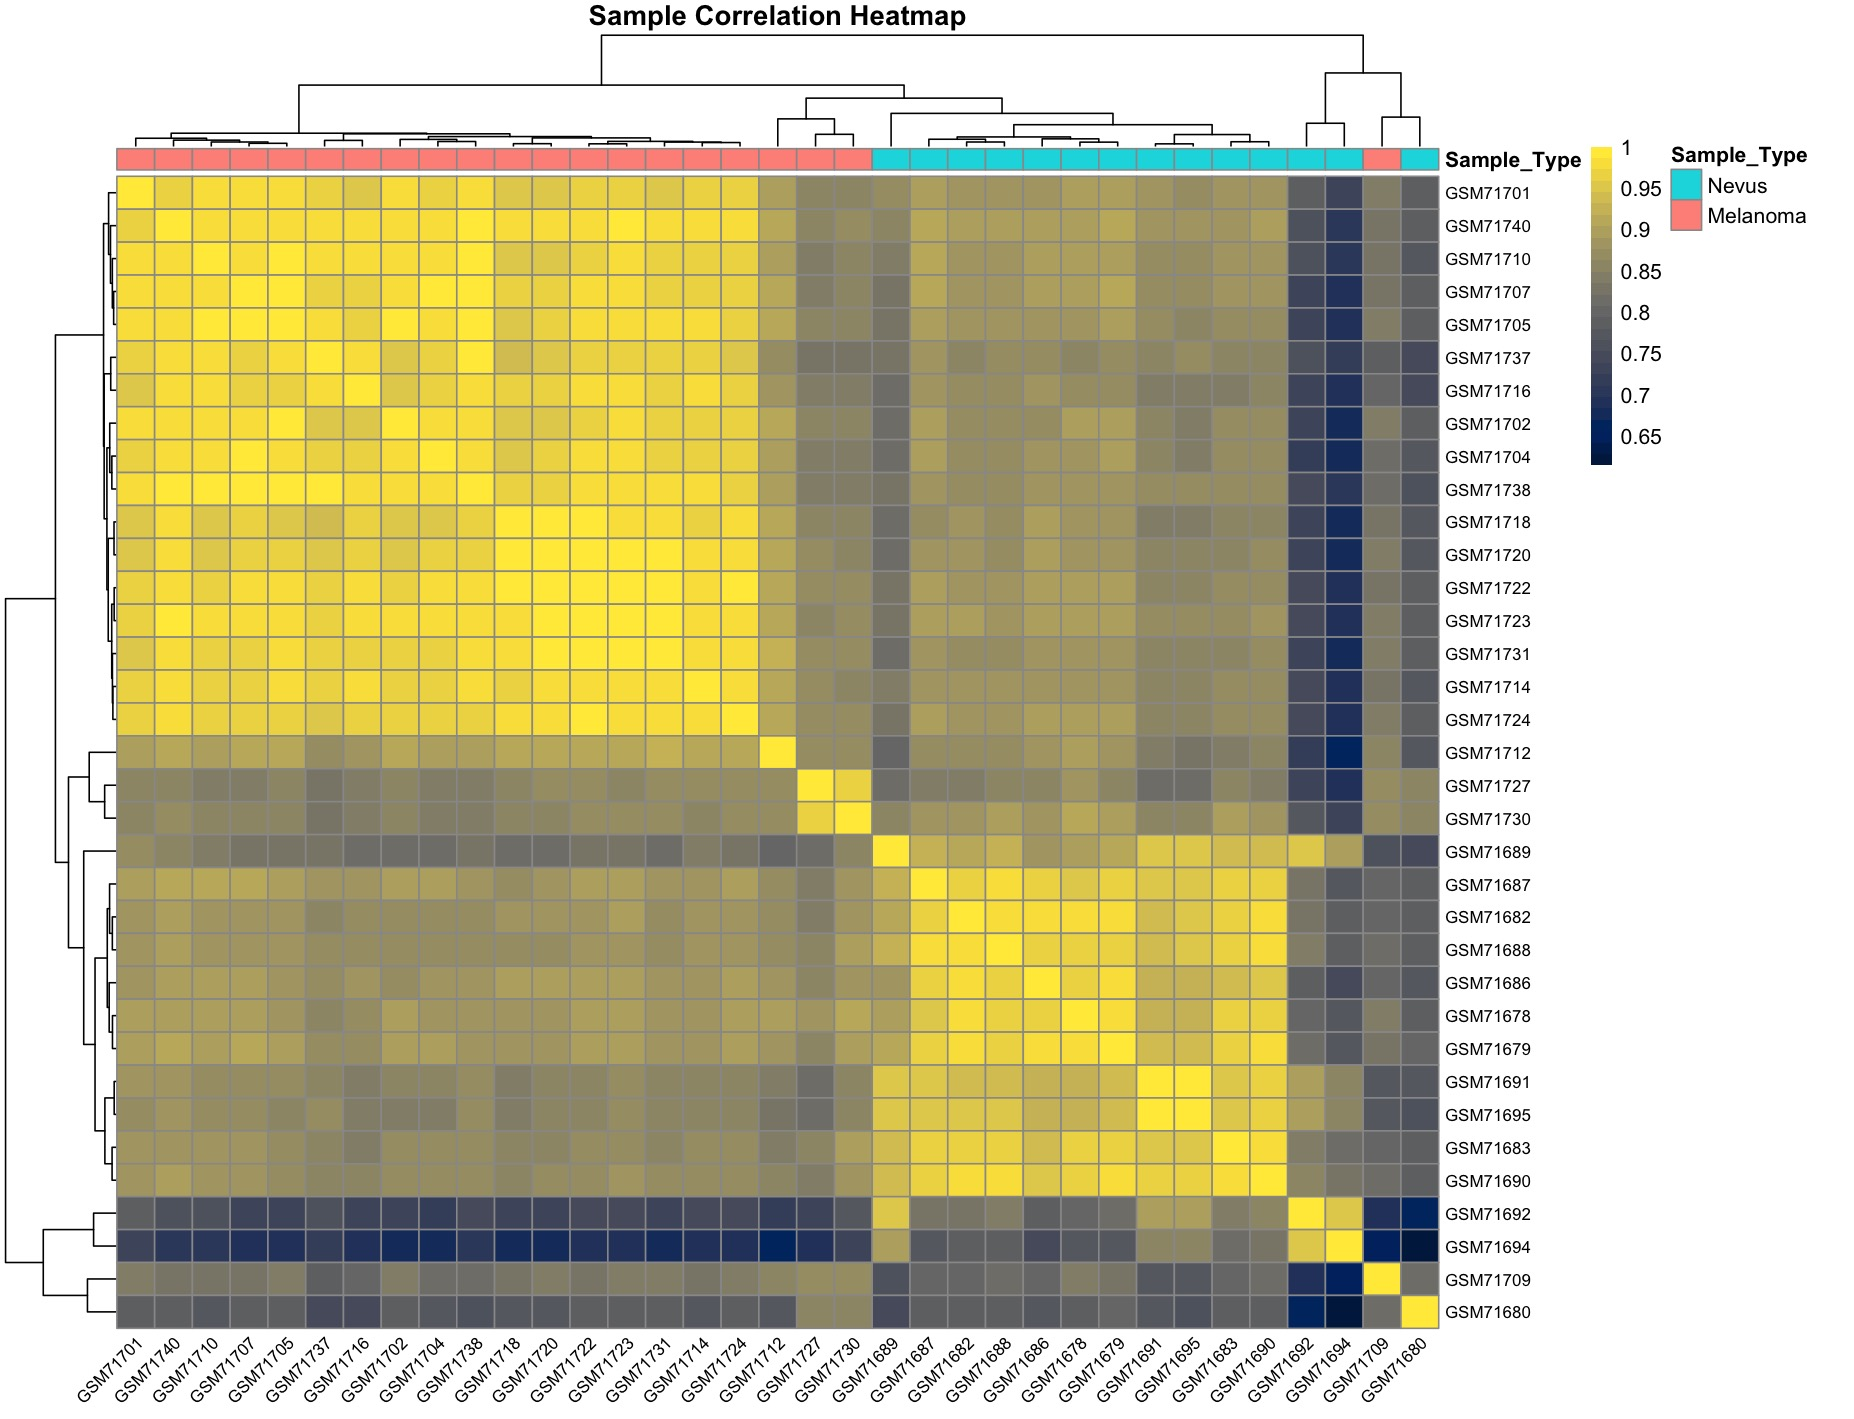
\includegraphics[width=1\linewidth]{Images/Heatmap} 

}

\caption{Sample Correlation Heatmap}\label{fig:unnamed-chunk-26}
\end{figure}

This heatmap shows the pairwise correlations between the samples in the
dataset.Yellow signifies a strong correlation and blue signifies no
correlation. The rows and columns represent the same set of samples.
Samples are hierarchically clustered based on their correlation. Similar
samples are grouped together. However, there is 1 melanoma sample that
is clustering with the nevi skin samples.

\subsubsection{Principal Component Analysis
(PCA)}\label{principal-component-analysis-pca}

\begin{figure}

{\centering 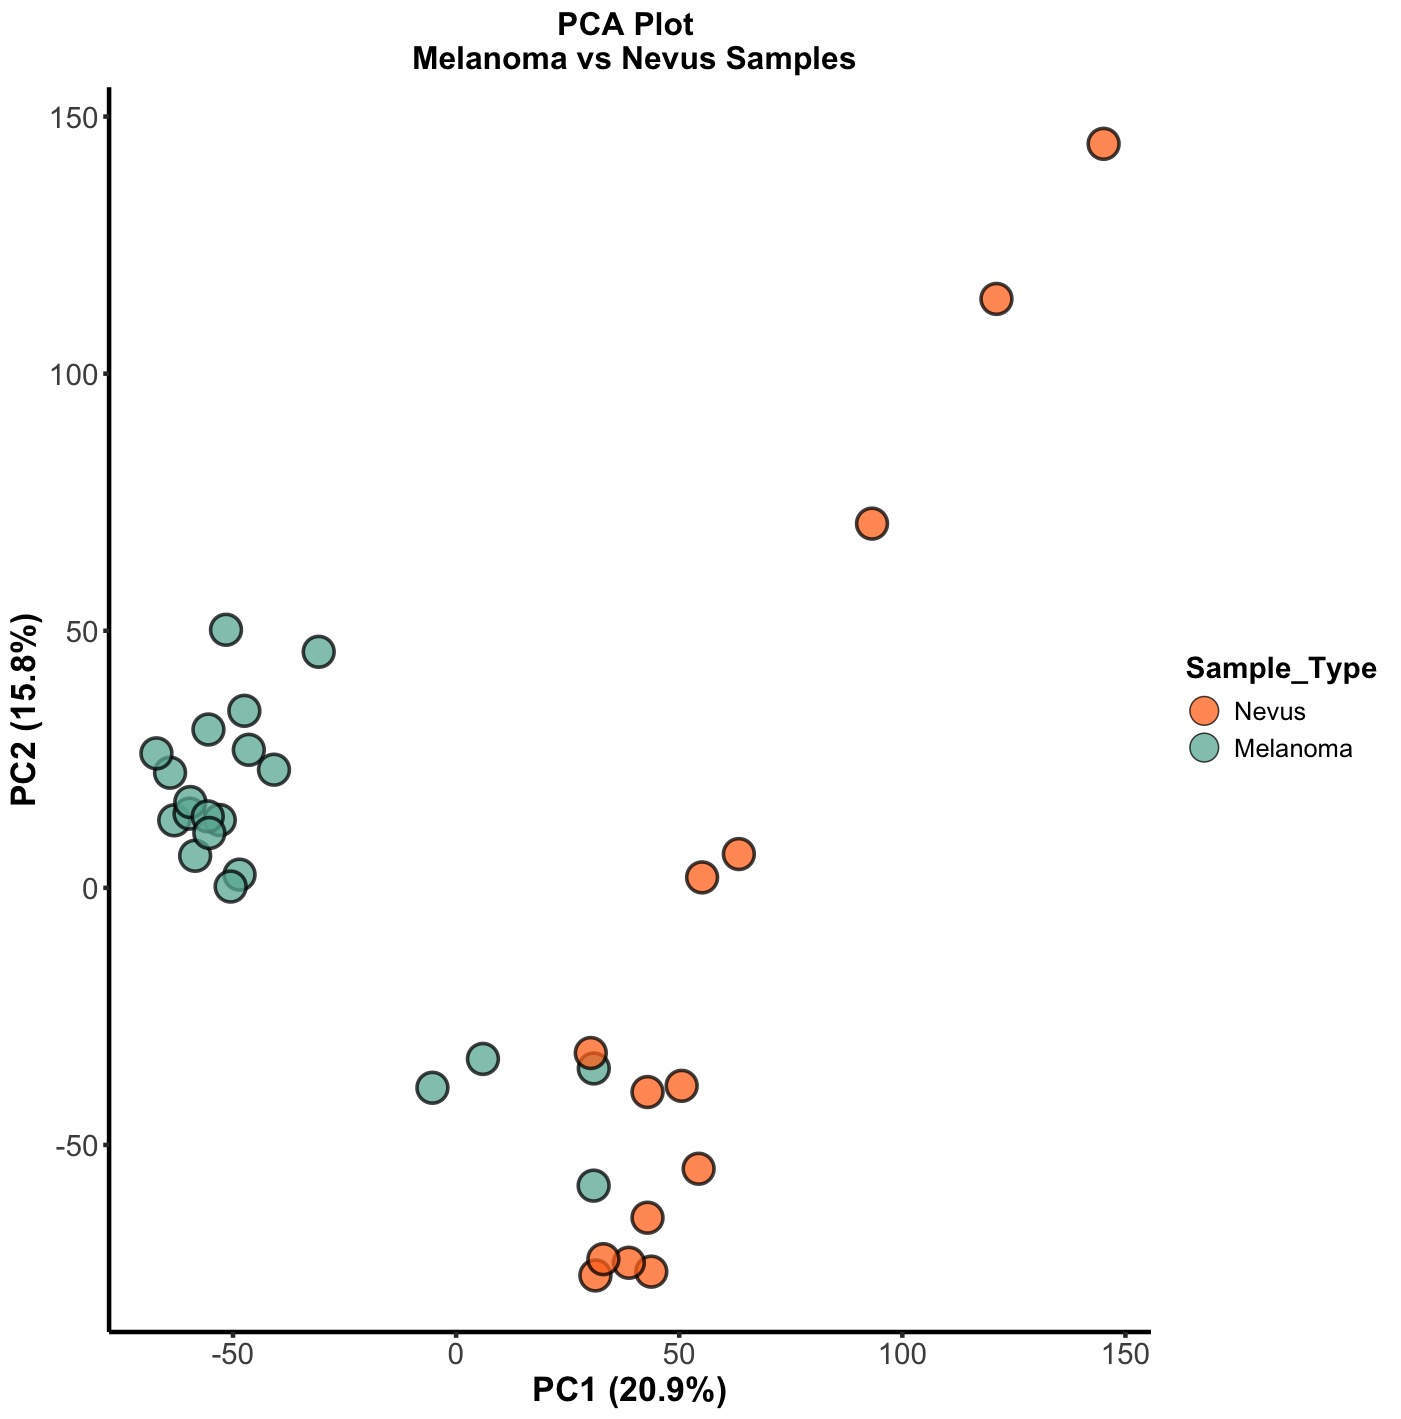
\includegraphics[width=0.6\linewidth]{Images/PCA_I.png} 

}

\caption{Principal Component Analysis (PCA)}\label{fig:unnamed-chunk-27}
\end{figure}

Principal Component Analysis (PCA) is a dimensionality reduction
technique used to simplify complex datasets by transforming correlated
variables into a smaller set of uncorrelated variables called principal
components.

\begin{figure}

{\centering 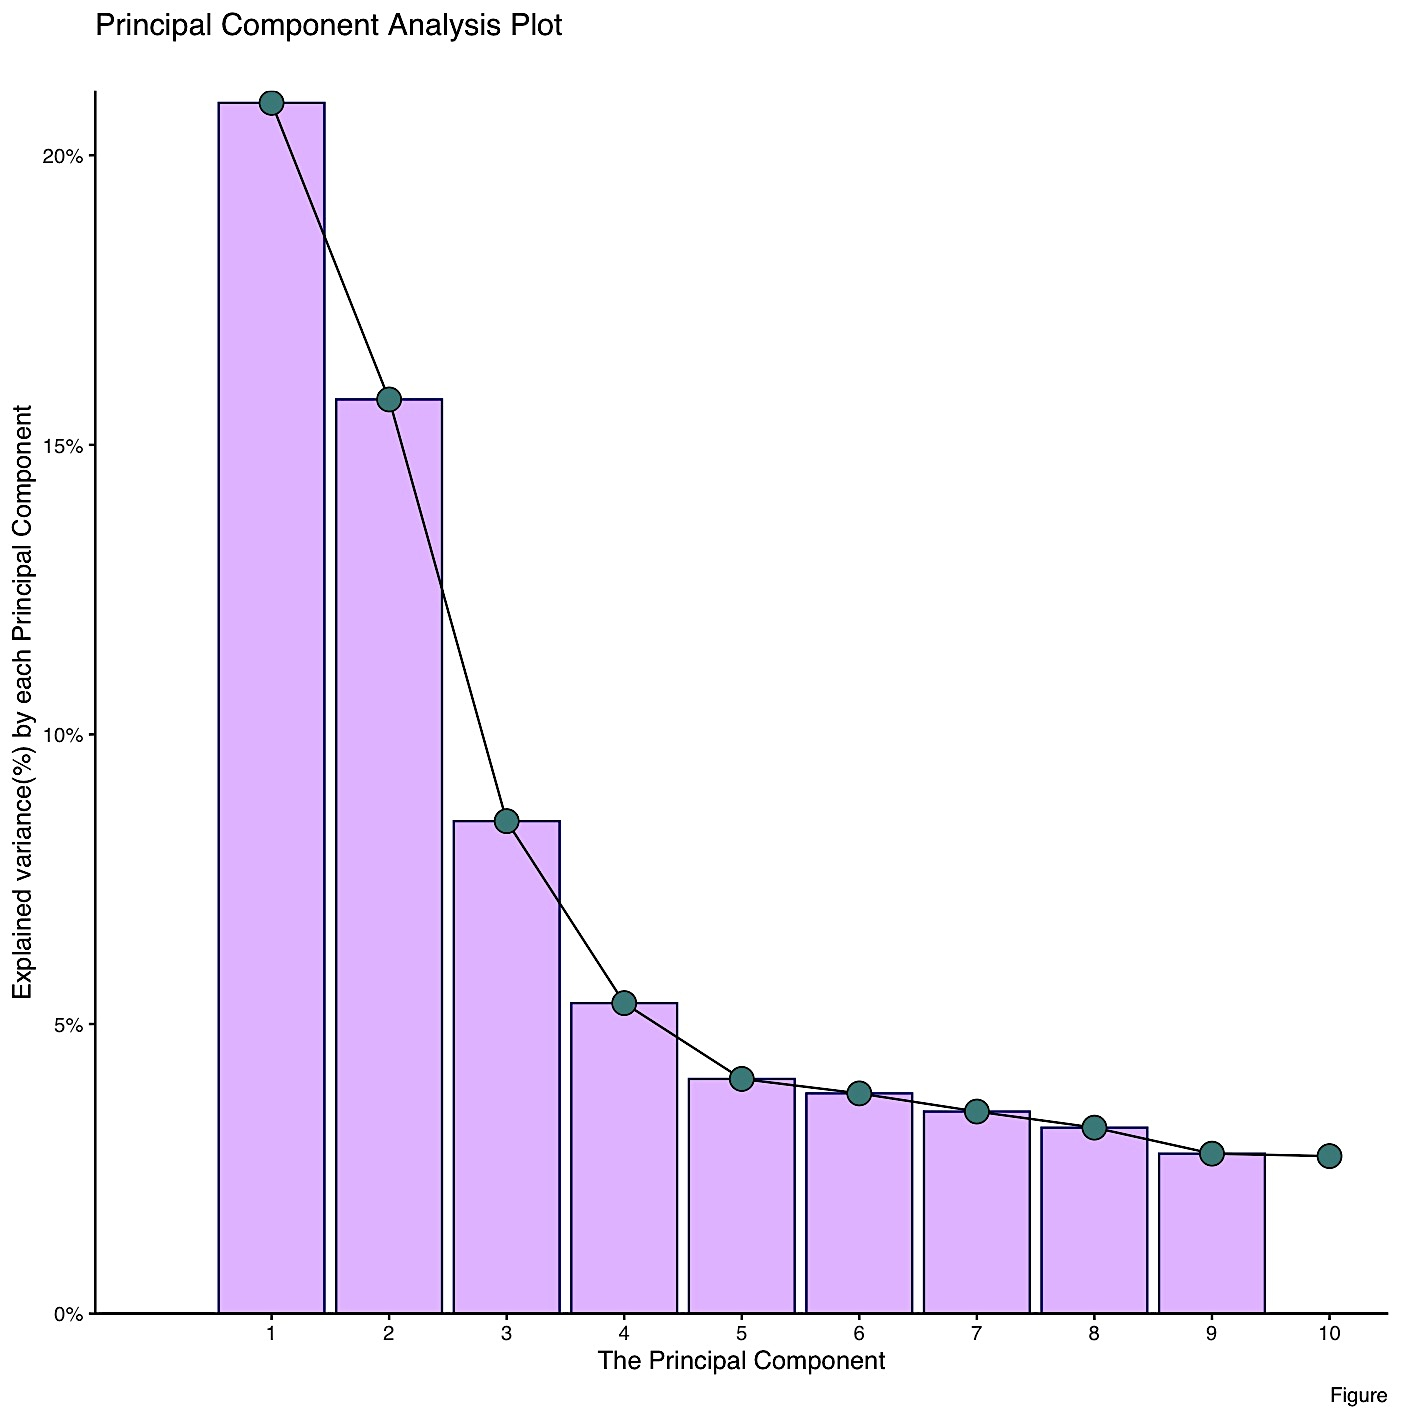
\includegraphics[width=0.5\linewidth]{Images/Scree.png} 

}

\caption{Scree Plot}\label{fig:unnamed-chunk-28}
\end{figure}
\newpage

\subsubsection{Uniform Manifold Approximation and Projection
(UMAP)}\label{uniform-manifold-approximation-and-projection-umap}

\begin{figure}

{\centering 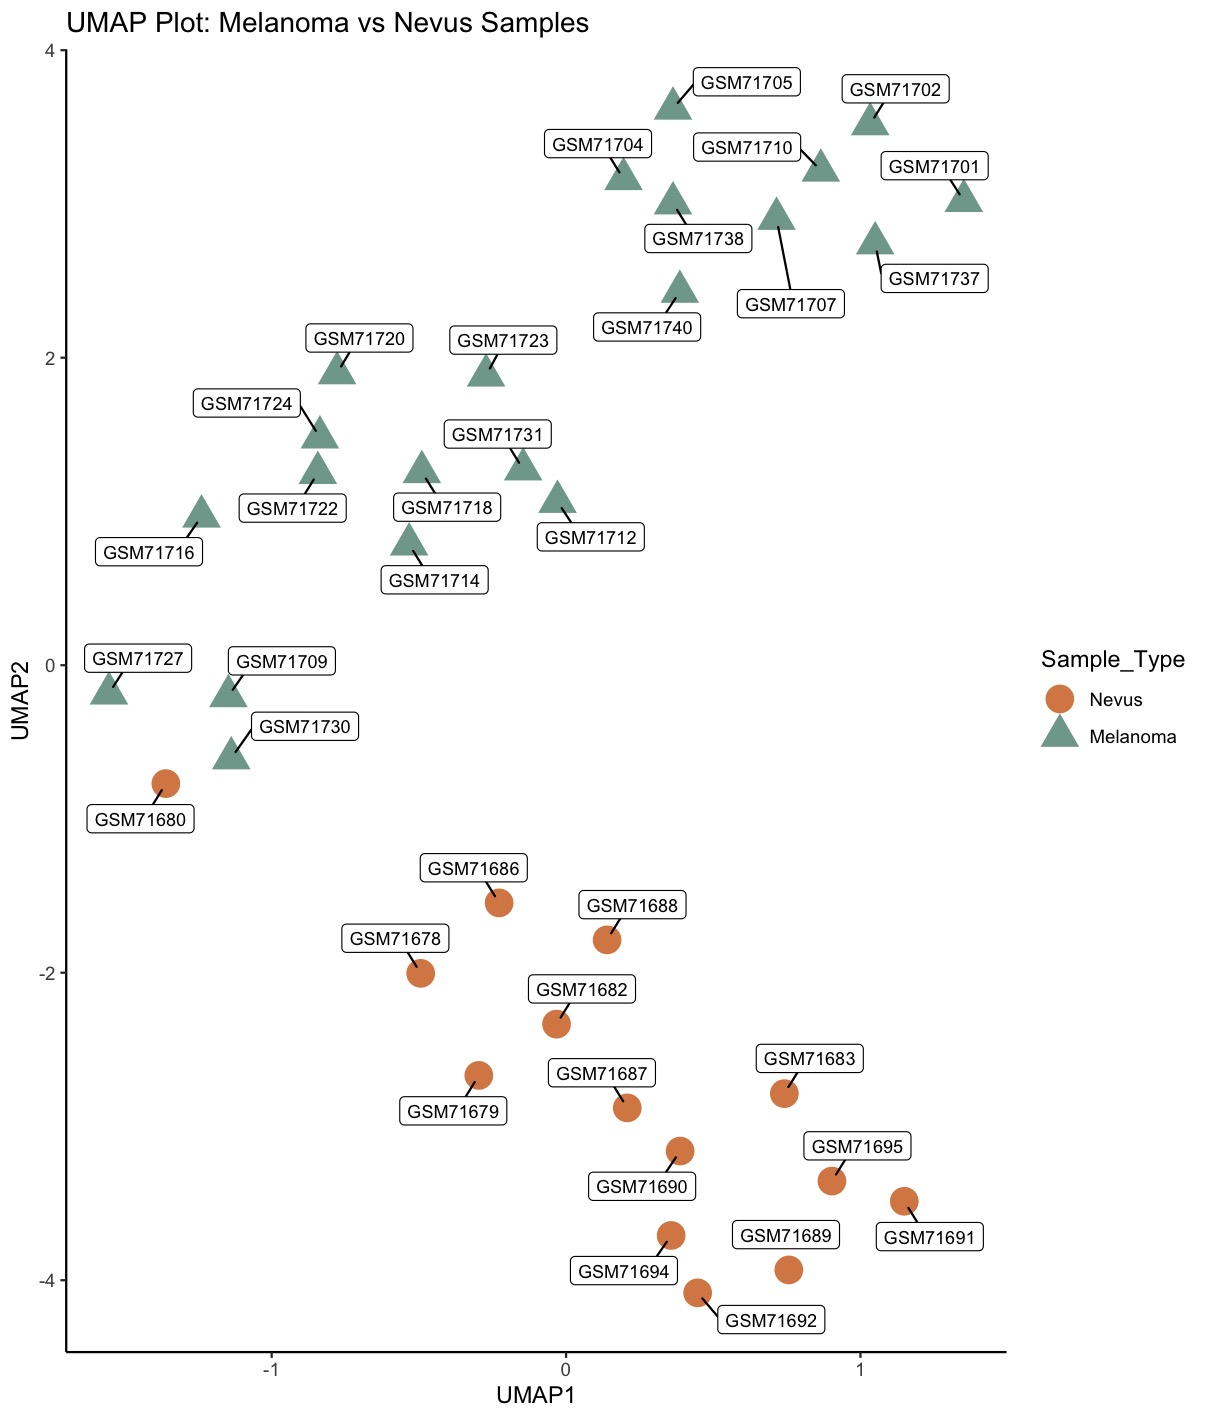
\includegraphics[width=0.8\linewidth]{Images/Umap} 

}

\caption{Uniform Manifold Approximation and Projection}\label{fig:unnamed-chunk-29}
\end{figure}

\newpage

\subsection{Pathway Analysis}\label{pathway-analysis}

KEGG / GO enrichment KEGG pathways identified to look at genes in
melanoma samples Biological Process and Pathway Analysis

The clusterProfiler package was used for pathway analysis.

\subsubsection{Top GO Biological
Processes}\label{top-go-biological-processes}

\begin{figure}

{\centering 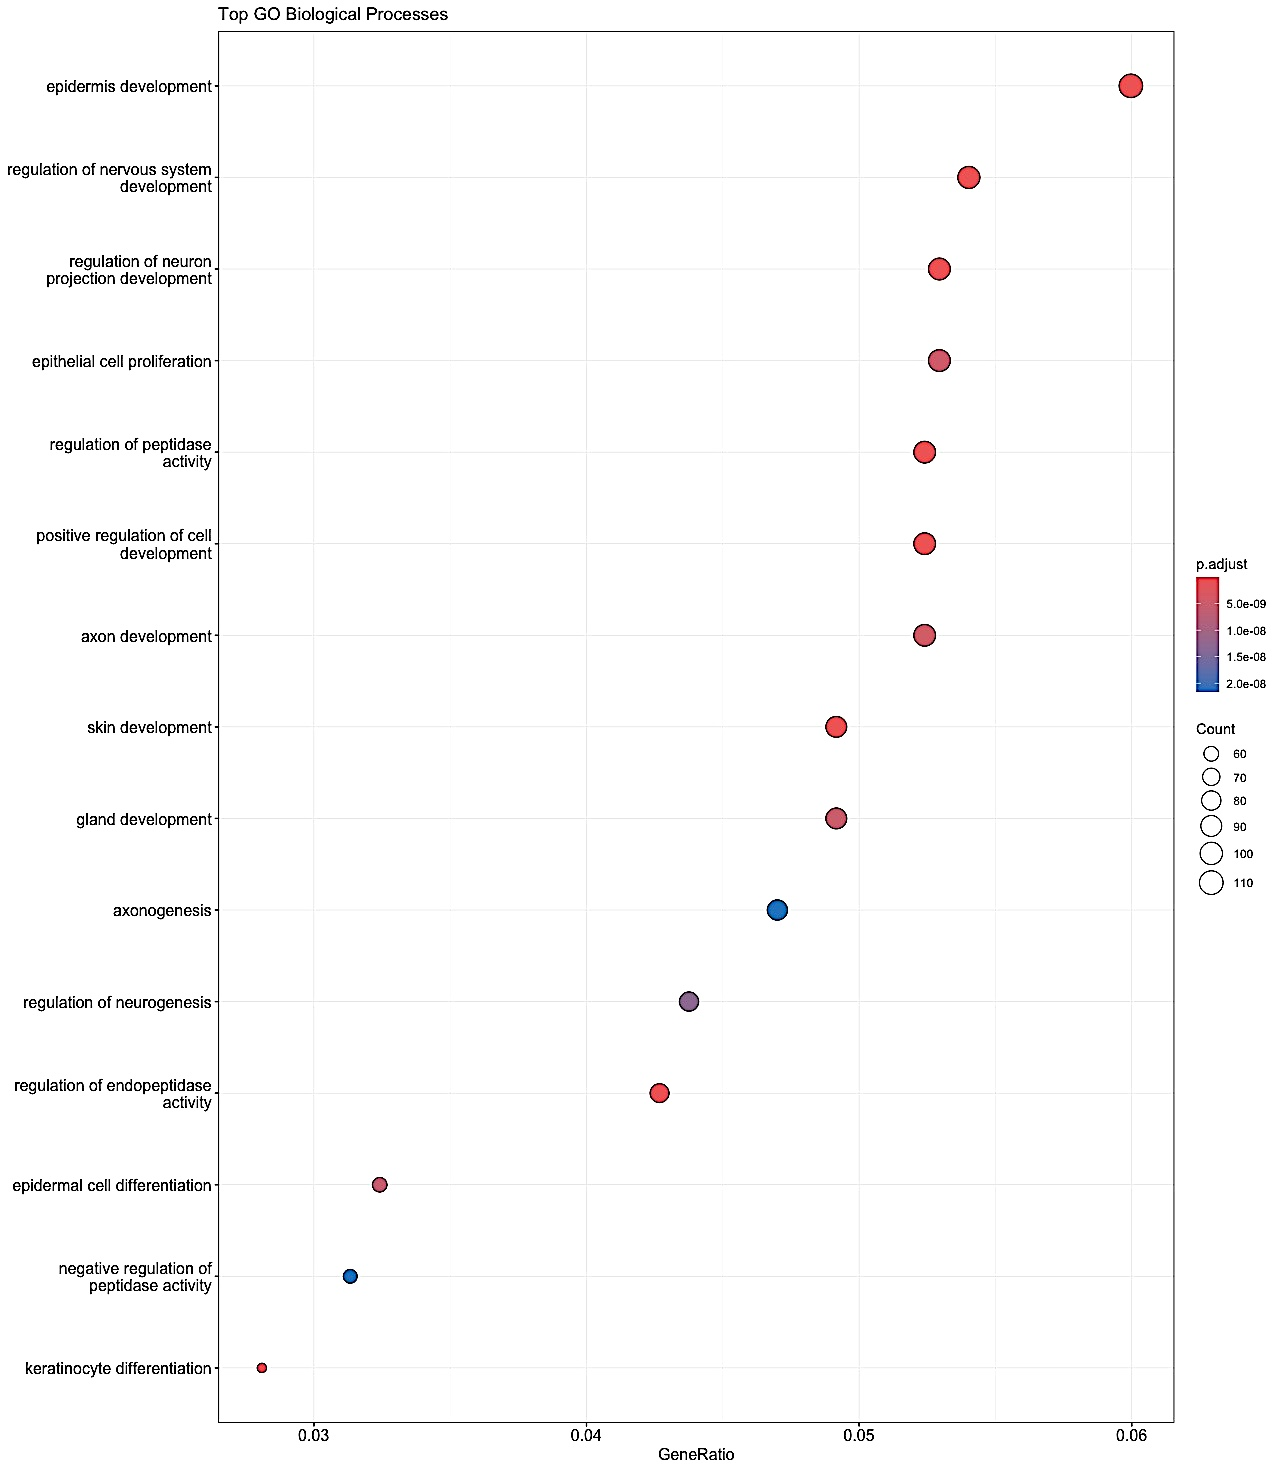
\includegraphics[width=0.8\linewidth]{Images/Top_GO_Biological_Processes} 

}

\caption{Gene Ontology Biological Processes}\label{fig:unnamed-chunk-30}
\end{figure}

\newpage

\subsubsection{Top KEGG Pathways}\label{top-kegg-pathways}

\begin{figure}

{\centering 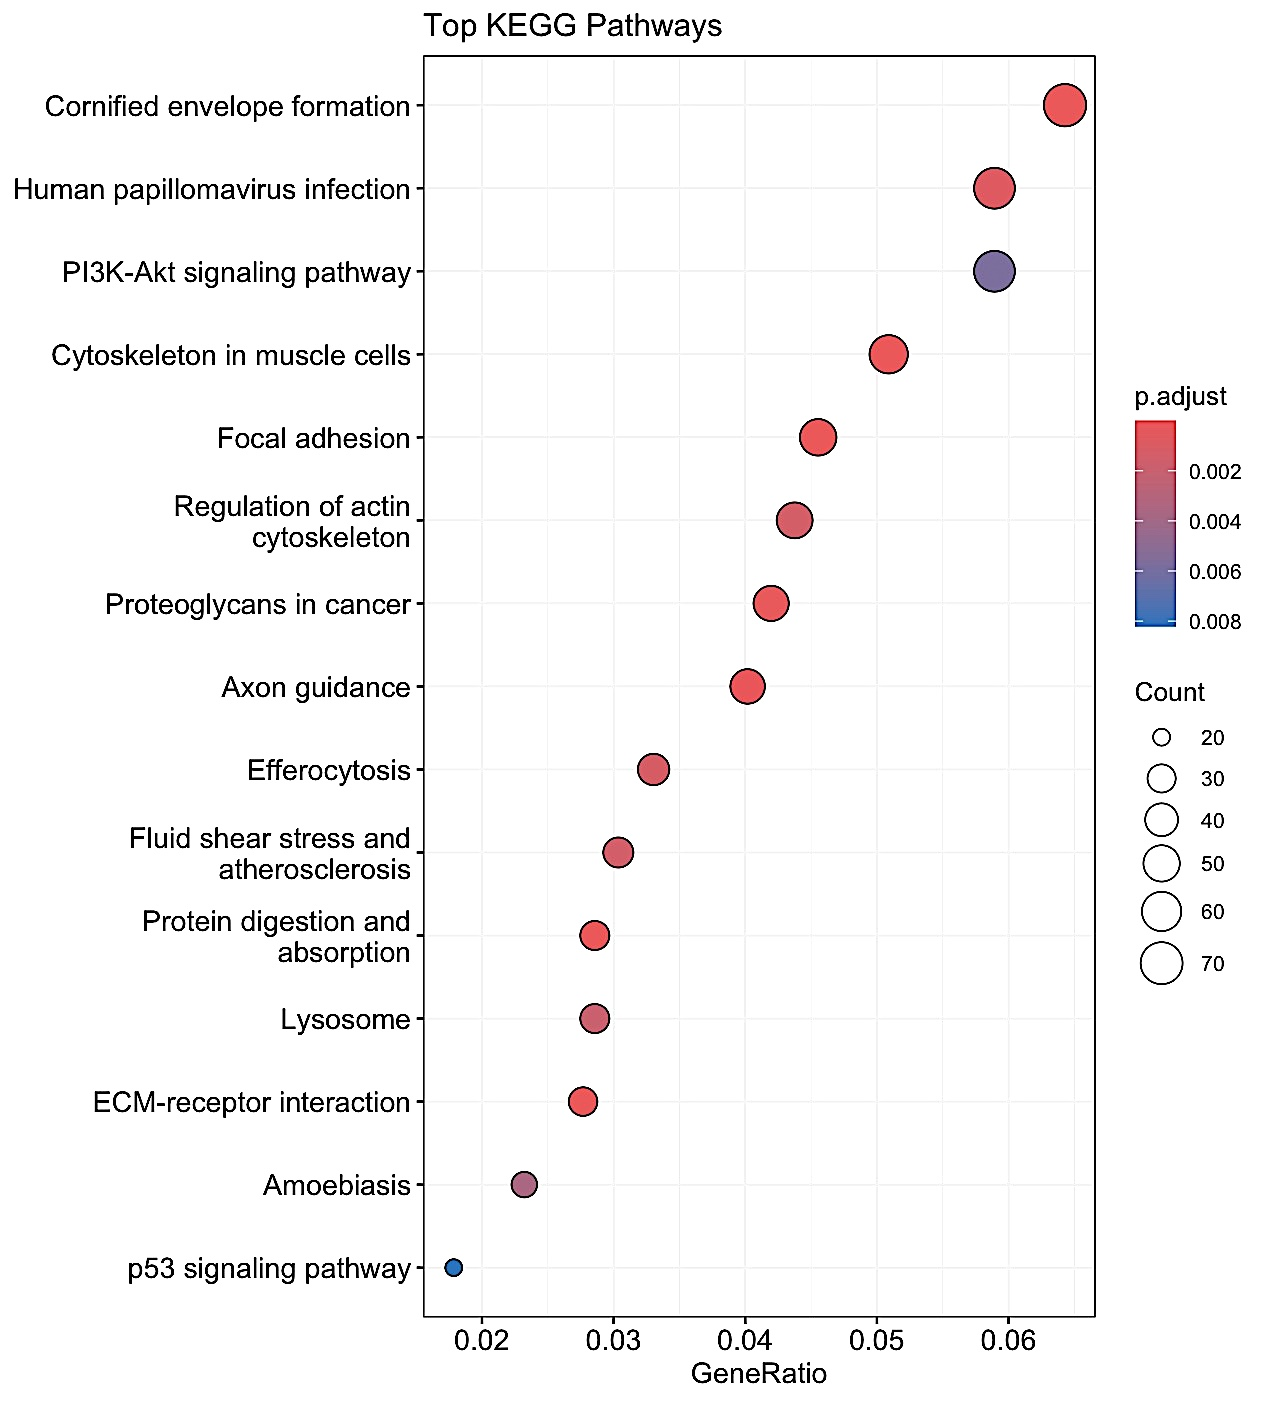
\includegraphics[width=0.8\linewidth]{Images/KEGG_pathways} 

}

\caption{KEGG Pathways}\label{fig:unnamed-chunk-31}
\end{figure}

\newpage

\subsection{Gene Signature Enrichment}\label{gene-signature-enrichment}

\begin{itemize}
\item
  GSVA / ssGSEA results
\item
  GSVA to perform ssGSEA analysis on signature genes with GSVA Package.
\end{itemize}

\begin{longtable}[]{@{}
  >{\raggedright\arraybackslash}p{(\columnwidth - 8\tabcolsep) * \real{0.1970}}
  >{\raggedright\arraybackslash}p{(\columnwidth - 8\tabcolsep) * \real{0.2197}}
  >{\raggedright\arraybackslash}p{(\columnwidth - 8\tabcolsep) * \real{0.1212}}
  >{\raggedright\arraybackslash}p{(\columnwidth - 8\tabcolsep) * \real{0.1364}}
  >{\raggedright\arraybackslash}p{(\columnwidth - 8\tabcolsep) * \real{0.3258}}@{}}
\caption{(ssGSEA Enrichment Summary)}\tabularnewline
\toprule\noalign{}
\begin{minipage}[b]{\linewidth}\raggedright
Gene Set
\end{minipage} & \begin{minipage}[b]{\linewidth}\raggedright
Mean Difference (Mel-Nevus)
\end{minipage} & \begin{minipage}[b]{\linewidth}\raggedright
P-value
\end{minipage} & \begin{minipage}[b]{\linewidth}\raggedright
Adjusted P-value
\end{minipage} & \begin{minipage}[b]{\linewidth}\raggedright
Significance
\end{minipage} \\
\midrule\noalign{}
\endfirsthead
\toprule\noalign{}
\begin{minipage}[b]{\linewidth}\raggedright
Gene Set
\end{minipage} & \begin{minipage}[b]{\linewidth}\raggedright
Mean Difference (Mel-Nevus)
\end{minipage} & \begin{minipage}[b]{\linewidth}\raggedright
P-value
\end{minipage} & \begin{minipage}[b]{\linewidth}\raggedright
Adjusted P-value
\end{minipage} & \begin{minipage}[b]{\linewidth}\raggedright
Significance
\end{minipage} \\
\midrule\noalign{}
\endhead
\bottomrule\noalign{}
\endlastfoot
Melanoma Upreg Top20 & 0.524 & 1.51e-14 & 4.53e-14 & Higher enrichment
in Melanoma \\
Melanoma Downreg Top20 & -0.7301 & 1.12e-10 & 1.68e-10 & Lower
enrichment in Melanoma \\
All Top DE Genes & -0.0661 & 1.08e-02 & 1.08e-02 & Lower enrichment in
Melanoma (small diff) \\
\end{longtable}

\begin{figure}

{\centering 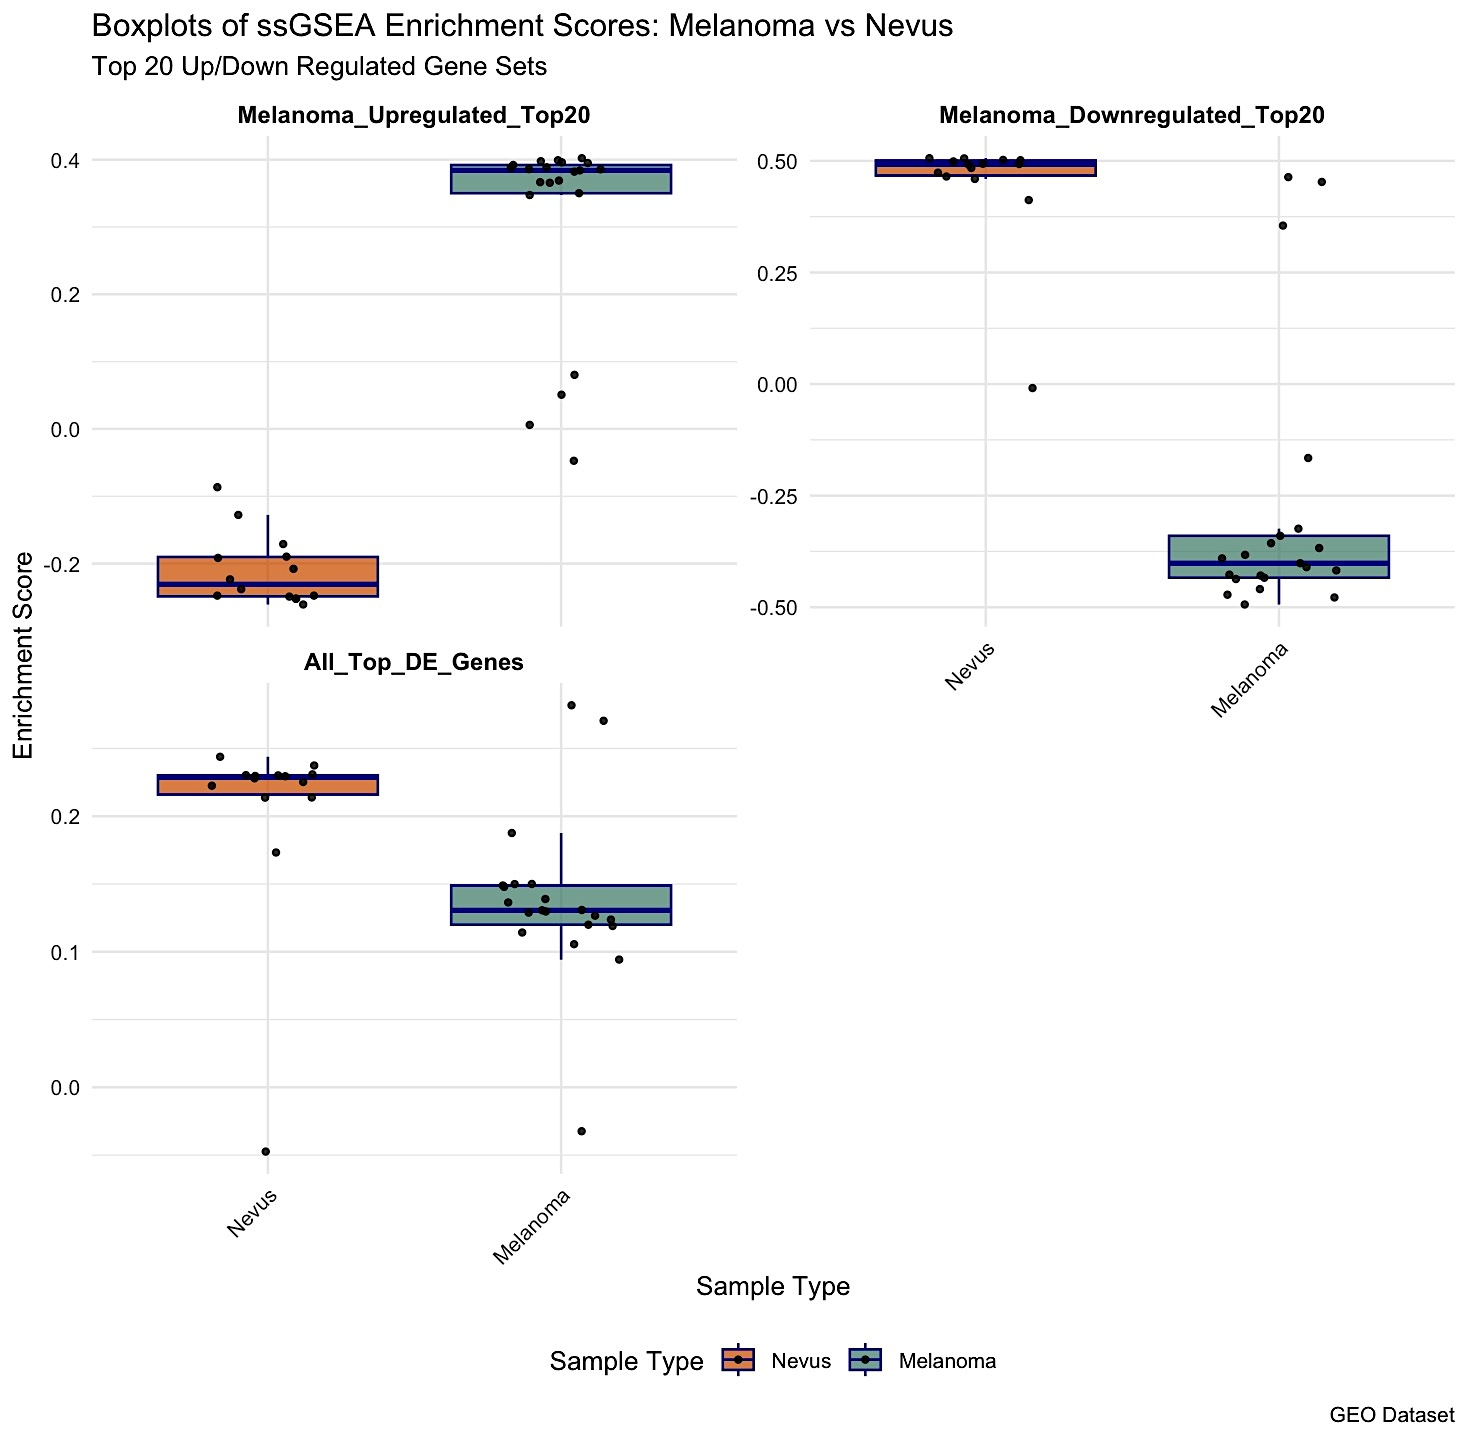
\includegraphics[width=0.8\linewidth]{Images/Boxplots of ssGSEA} 

}

\caption{ssGSEA Enrichment Scoress}\label{fig:unnamed-chunk-32}
\end{figure}

\begin{figure}

{\centering 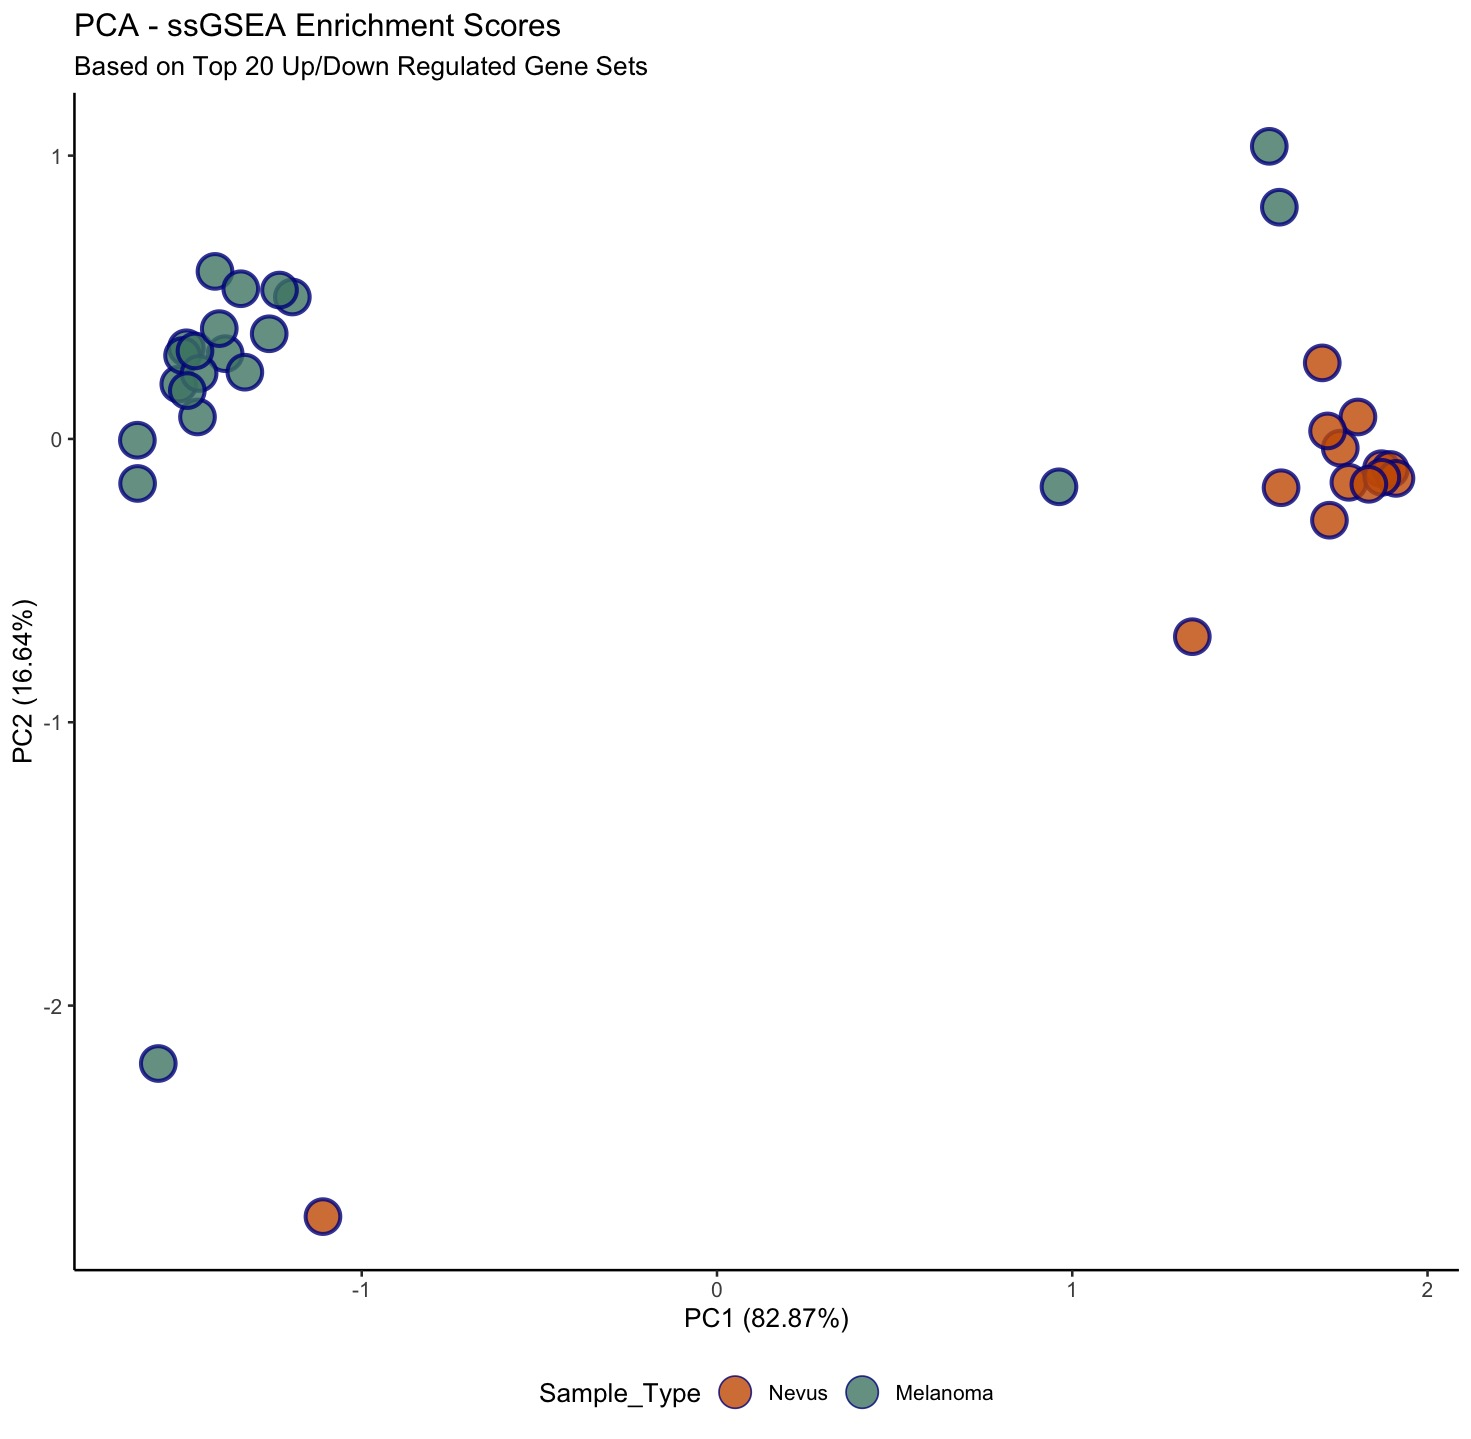
\includegraphics[width=0.9\linewidth]{Images/ssGSEA_PCA} 

}

\caption{PCA from GSVA}\label{fig:unnamed-chunk-33}
\end{figure}

\newpage

\subsection{Tumor Purity Estimation for Melanoma vs Nevus
Samples}\label{tumor-purity-estimation-for-melanoma-vs-nevus-samples}

\begin{longtable}[]{@{}llll@{}}
\caption{(ESTIMATE Score Comparison: Melanoma vs Nevus)}\tabularnewline
\toprule\noalign{}
Score & Melanoma\_Mean & Nevus\_Mean & P\_Value \\
\midrule\noalign{}
\endfirsthead
\toprule\noalign{}
Score & Melanoma\_Mean & Nevus\_Mean & P\_Value \\
\midrule\noalign{}
\endhead
\bottomrule\noalign{}
\endlastfoot
StromalScore & -602.188 & -486.441 & 0.6347 \\
ImmuneScore & -302.864 & -505.272 & 0.5063 \\
ESTIMATEScore & -905.052 & -991.713 & 0.8710 \\
TumorPurity & 0.869 & 0.879 & 0.8334 \\
\end{longtable}

\begin{figure}

{\centering 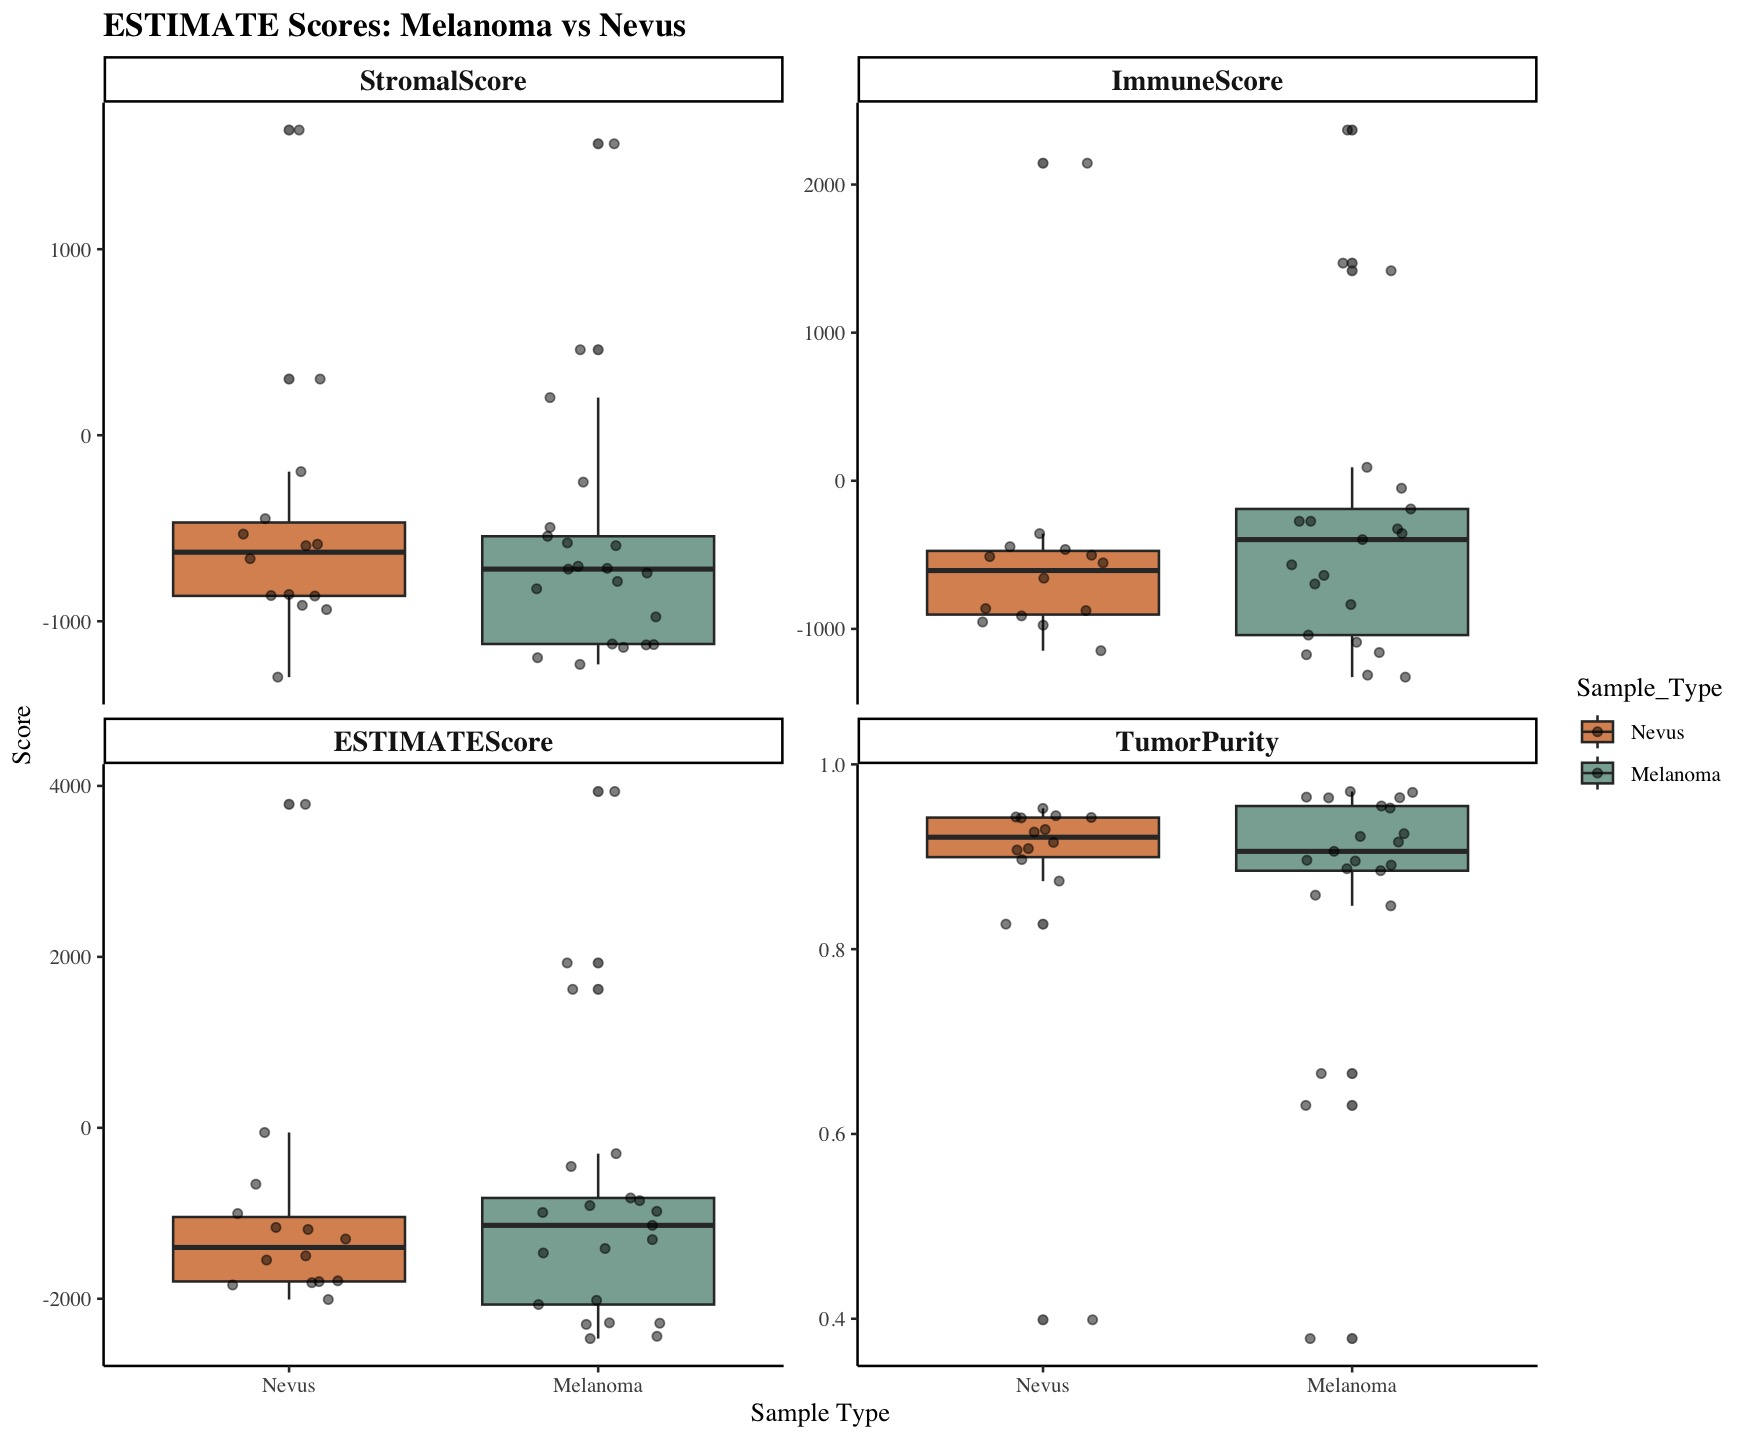
\includegraphics[width=0.9\linewidth]{Images/ESTIMATE} 

}

\caption{ESTIMATE Scores}\label{fig:unnamed-chunk-34}
\end{figure}

\newpage

\section{RESULTS -- Topic II: Streptococcus
pyogenes}\label{results-topic-ii-streptococcus-pyogenes}

\subsubsection{Sequence Dataset
Overview}\label{sequence-dataset-overview}

Summary table of GAS strains and emm genes.

\begin{longtable}[]{@{}
  >{\raggedright\arraybackslash}p{(\columnwidth - 8\tabcolsep) * \real{0.1238}}
  >{\raggedright\arraybackslash}p{(\columnwidth - 8\tabcolsep) * \real{0.1524}}
  >{\raggedright\arraybackslash}p{(\columnwidth - 8\tabcolsep) * \real{0.0952}}
  >{\raggedright\arraybackslash}p{(\columnwidth - 8\tabcolsep) * \real{0.1619}}
  >{\raggedright\arraybackslash}p{(\columnwidth - 8\tabcolsep) * \real{0.4667}}@{}}
\caption{(Table of \emph{Streptococcus pyogenes}
genomes)}\tabularnewline
\toprule\noalign{}
\begin{minipage}[b]{\linewidth}\raggedright
Name.
\end{minipage} & \begin{minipage}[b]{\linewidth}\raggedright
Accession Number
\end{minipage} & \begin{minipage}[b]{\linewidth}\raggedright
Strain
\end{minipage} & \begin{minipage}[b]{\linewidth}\raggedright
Collection Date
\end{minipage} & \begin{minipage}[b]{\linewidth}\raggedright
Link
\end{minipage} \\
\midrule\noalign{}
\endfirsthead
\toprule\noalign{}
\begin{minipage}[b]{\linewidth}\raggedright
Name.
\end{minipage} & \begin{minipage}[b]{\linewidth}\raggedright
Accession Number
\end{minipage} & \begin{minipage}[b]{\linewidth}\raggedright
Strain
\end{minipage} & \begin{minipage}[b]{\linewidth}\raggedright
Collection Date
\end{minipage} & \begin{minipage}[b]{\linewidth}\raggedright
Link
\end{minipage} \\
\midrule\noalign{}
\endhead
\bottomrule\noalign{}
\endlastfoot
S. Pyogenes & AE014074.1 & MGAS315 & 31-JAN-2014 &
\url{https://www.ncbi.nlm.nih.gov/nuccore/AE014074.1} \\
S. Pyogenes & CP000017.2 & MGAS5005 & 01-APR-2014 &
\url{https://www.ncbi.nlm.nih.gov/nuccore/CP000017.2} \\
S. Pyogenes & CP155740.1 & 1851/03 & 06-AUG-2024 &
\url{https://www.ncbi.nlm.nih.gov/nuccore/CP155740.1} \\
\end{longtable}

\begin{longtable}[]{@{}
  >{\raggedright\arraybackslash}p{(\columnwidth - 6\tabcolsep) * \real{0.1650}}
  >{\raggedright\arraybackslash}p{(\columnwidth - 6\tabcolsep) * \real{0.2524}}
  >{\raggedright\arraybackslash}p{(\columnwidth - 6\tabcolsep) * \real{0.1165}}
  >{\raggedright\arraybackslash}p{(\columnwidth - 6\tabcolsep) * \real{0.4660}}@{}}
\caption{(Table of \emph{Streptococcus pyogenes} emm genes)
\emph{Streptococcus pyogenes} emm gene for M protein, complete cds of
various strains -- Collection Date: 15-JAN-2014}\tabularnewline
\toprule\noalign{}
\begin{minipage}[b]{\linewidth}\raggedright
Accession Number
\end{minipage} & \begin{minipage}[b]{\linewidth}\raggedright
Gene Name
\end{minipage} & \begin{minipage}[b]{\linewidth}\raggedright
Strain
\end{minipage} & \begin{minipage}[b]{\linewidth}\raggedright
Link
\end{minipage} \\
\midrule\noalign{}
\endfirsthead
\toprule\noalign{}
\begin{minipage}[b]{\linewidth}\raggedright
Accession Number
\end{minipage} & \begin{minipage}[b]{\linewidth}\raggedright
Gene Name
\end{minipage} & \begin{minipage}[b]{\linewidth}\raggedright
Strain
\end{minipage} & \begin{minipage}[b]{\linewidth}\raggedright
Link
\end{minipage} \\
\midrule\noalign{}
\endhead
\bottomrule\noalign{}
\endlastfoot
AB548437.1 & emm1 gene for M protein & RE014 &
\url{https://www.ncbi.nlm.nih.gov/nuccore/AB548437.1} \\
AB548438.1 & emm28 gene for M protein & RE015 &
\url{https://www.ncbi.nlm.nih.gov/nuccore/AB548438.1} \\
AB548441.1 & emm1 gene for M protein & RE020 &
\url{https://www.ncbi.nlm.nih.gov/nuccore/AB548441.1} \\
AB548442.1 & emm1 gene for M protein & RE025 &
\url{https://www.ncbi.nlm.nih.gov/nuccore/AB548442.1} \\
AB548444.1 & emm28 gene for M protein & RE031 &
\url{https://www.ncbi.nlm.nih.gov/nuccore/AB548444.1} \\
AB548445.1 & emm1 gene for M protein & RE032 &
\url{https://www.ncbi.nlm.nih.gov/nuccore/AB548445.1} \\
AB548446.1 & emm49 gene for M protein & RE037 &
\url{https://www.ncbi.nlm.nih.gov/nuccore/AB548446.1} \\
AB548447.1 & emm49 gene for M protein & RE039 &
\url{https://www.ncbi.nlm.nih.gov/nuccore/AB548447.1} \\
AB548448.1 & emm28 gene for M protein & RE041 &
\url{https://www.ncbi.nlm.nih.gov/nuccore/AB548448.1} \\
AB548449.1 & emm89 gene for M protein & RE050 &
\url{https://www.ncbi.nlm.nih.gov/nuccore/AB548449.1} \\
AB548450.1 & emm1 gene for M protein & RE059 &
\url{https://www.ncbi.nlm.nih.gov/nuccore/AB548450.1} \\
AB548451.1 & emm12 gene for M protein & RE066 &
\url{https://www.ncbi.nlm.nih.gov/nuccore/AB548451.1} \\
AB548452.1 & emm49 gene for M protein & RE076 &
\url{https://www.ncbi.nlm.nih.gov/nuccore/AB548452.1} \\
AB548453.1 & emm49 gene for M protein & RE080 &
\url{https://www.ncbi.nlm.nih.gov/nuccore/AB548453.1} \\
AB548454.1 & emm49 gene for M protein & RE104 &
\url{https://www.ncbi.nlm.nih.gov/nuccore/AB548454.1} \\
AB548456.1 & emm49 gene for M protein & RE121 &
\url{https://www.ncbi.nlm.nih.gov/nuccore/AB548456.1} \\
AB548503.1 & emm4 gene for M protein & RE342 &
\url{https://www.ncbi.nlm.nih.gov/nuccore/AB548503.1} \\
AB548508.1 & emm12 gene for M protein & RE366 &
\url{https://www.ncbi.nlm.nih.gov/nuccore/AB548508.1} \\
AB548516.1 & emm75 gene for M protein & RE436 &
\url{https://www.ncbi.nlm.nih.gov/nuccore/AB548516.1} \\
AB549960.1 & emm58 gene for M protein & RE614 &
\url{https://www.ncbi.nlm.nih.gov/nuccore/AB549960.1} \\
\end{longtable}

\begin{longtable}[]{@{}
  >{\raggedright\arraybackslash}p{(\columnwidth - 6\tabcolsep) * \real{0.1717}}
  >{\raggedright\arraybackslash}p{(\columnwidth - 6\tabcolsep) * \real{0.2222}}
  >{\raggedright\arraybackslash}p{(\columnwidth - 6\tabcolsep) * \real{0.1212}}
  >{\raggedright\arraybackslash}p{(\columnwidth - 6\tabcolsep) * \real{0.4848}}@{}}
\caption{(Outgroup: \emph{Streptococcus pyogenes} emm50 type - emm gene
for M protein, partial cds. of various strains -- Collection Date:
26-JUN-2013}\tabularnewline
\toprule\noalign{}
\begin{minipage}[b]{\linewidth}\raggedright
Accession Number
\end{minipage} & \begin{minipage}[b]{\linewidth}\raggedright
Gene Name
\end{minipage} & \begin{minipage}[b]{\linewidth}\raggedright
Strain
\end{minipage} & \begin{minipage}[b]{\linewidth}\raggedright
Link
\end{minipage} \\
\midrule\noalign{}
\endfirsthead
\toprule\noalign{}
\begin{minipage}[b]{\linewidth}\raggedright
Accession Number
\end{minipage} & \begin{minipage}[b]{\linewidth}\raggedright
Gene Name
\end{minipage} & \begin{minipage}[b]{\linewidth}\raggedright
Strain
\end{minipage} & \begin{minipage}[b]{\linewidth}\raggedright
Link
\end{minipage} \\
\midrule\noalign{}
\endhead
\bottomrule\noalign{}
\endlastfoot
JX028641.1 & emm gene, emm50 type & GLS244 &
\url{https://www.ncbi.nlm.nih.gov/nuccore/JX028641} \\
\end{longtable}

\newpage

\subsection{Phylogenetic Analysis using
PAUP}\label{phylogenetic-analysis-using-paup}

The FASTA-formatted gene sequences were initially downloaded and
subsequently renamed according to a standardised naming convention,
incoporating the strain identifier, Genbank accession number, and gene
name. This nomenclature facilitated consistency and traceability
throughout the downstream analysis.

The individual FASTA files were concatenated into a single file using a
Bash shell command as shown below:

\begin{Shaded}
\begin{Highlighting}[]
\FunctionTok{cat} \PreprocessorTok{*} \OperatorTok{\textgreater{}}\NormalTok{ ../emm.fasta}
\end{Highlighting}
\end{Shaded}

The resulting emm.fasta file was then opened in AliView for inspection
and manual verification. During this process sequence headers were
further edited to ensure uniqueness and clarity.

To perform multiple sequence alignment , the software \textbf{MUSCLE}
was employed using the following command:

\begin{Shaded}
\begin{Highlighting}[]
\ExtensionTok{muscle} \AttributeTok{{-}in}\NormalTok{ emm.fasta }\AttributeTok{{-}out}\NormalTok{ emm\_aligned.fasta}
\end{Highlighting}
\end{Shaded}

The aligned sequences (emm\_aligned.fasta) were again viewed in AliView
to assessalignment quality and make any necessary further
adjustments\textsuperscript{28}.

\begin{figure}

{\centering 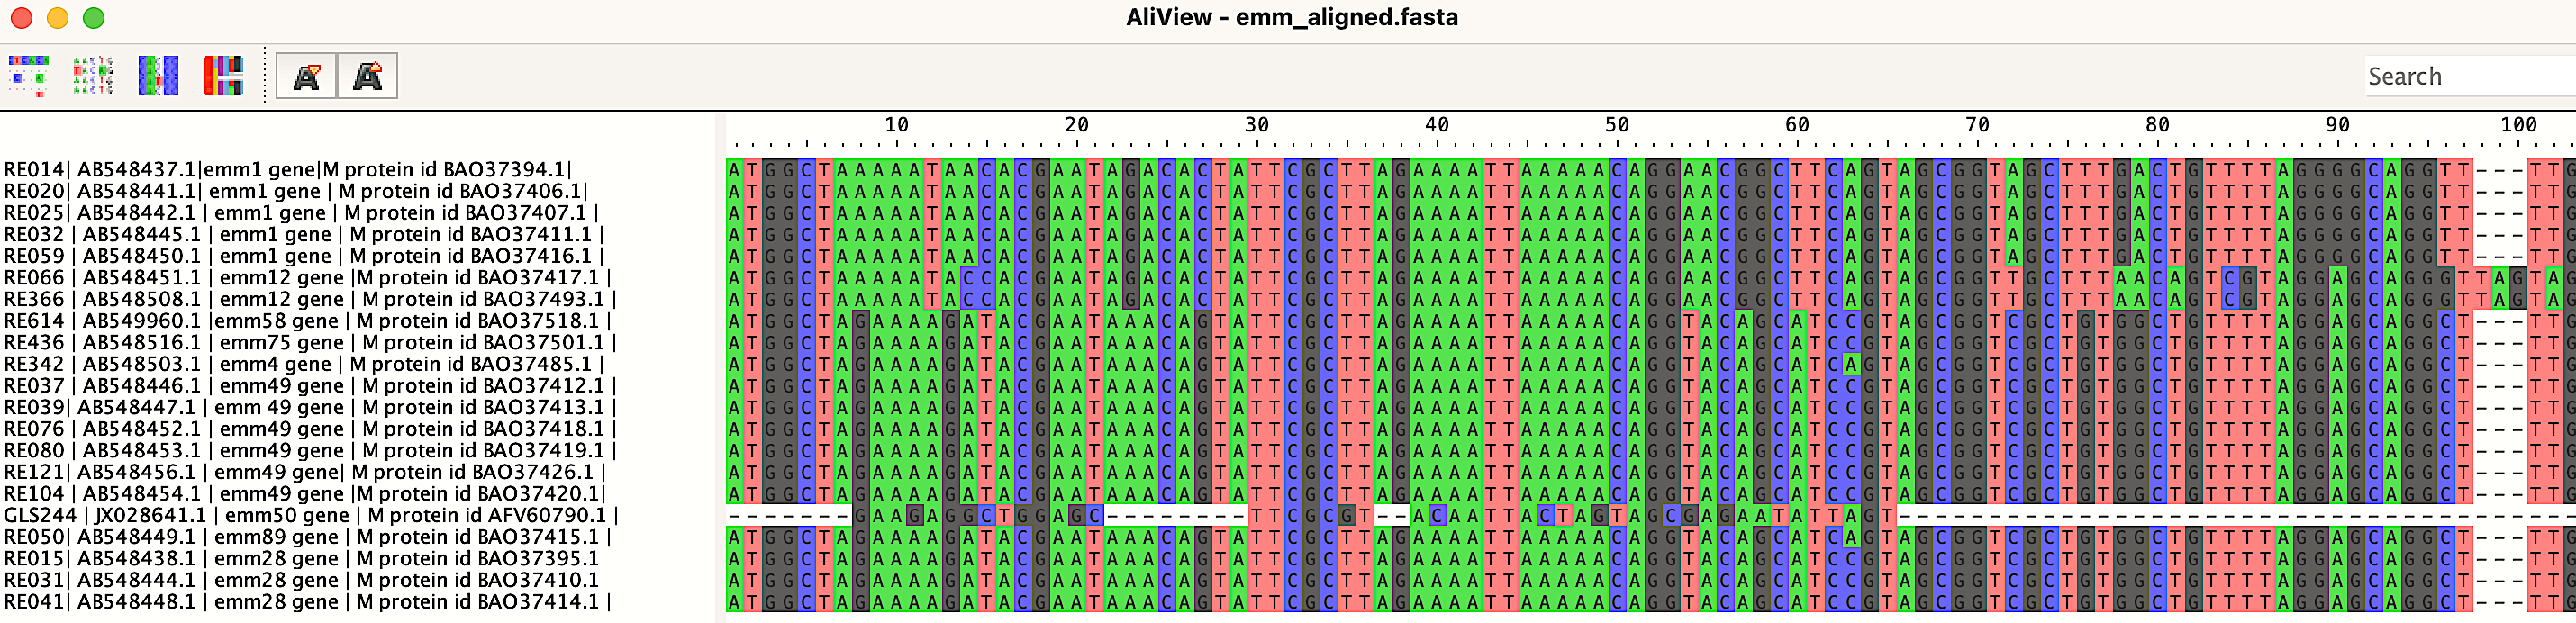
\includegraphics[width=1\linewidth]{Images/AliView} 

}

\caption{AliView}\label{fig:unnamed-chunk-37}
\end{figure}

Following alignment the file was converted into NEXUS format for
phylogenetic analysis using a custom Python script
\texttt{seqconverter.py}\textsuperscript{29} in conjuction with the
\texttt{sequenclib.py} .

The phylogenetic analysis was carried out in PAUP*
software\textsuperscript{30} using the sequence labelled as GLS244 as
the designated outgroup.

\begin{Shaded}
\begin{Highlighting}[]
\ExtensionTok{PAUP}
\ExtensionTok{execute}\NormalTok{ emm.nexus}
\ExtensionTok{showmatrix}
\ExtensionTok{outgroup}\NormalTok{  GLS244}
\end{Highlighting}
\end{Shaded}

A consensus tree was subsequently generated and visualised using
\textbf{FigTree}\textsuperscript{31}, allowing for a clear
interpretation of the evolutionary relationships among the sampled
strains.

\begin{Shaded}
\begin{Highlighting}[]
\BuiltInTok{set}\NormalTok{ root=outgroup outroot=monophyl}
\ExtensionTok{contree}\NormalTok{ all /strict=no majrule=yes percent=50}
\ExtensionTok{savetrees}\NormalTok{ from=1 to=1 file=consensus\_tree.tre format=newick brlens=yes}\KeywordTok{;}
\ExtensionTok{figtree}\NormalTok{ consensus\_tree.tre}
\end{Highlighting}
\end{Shaded}

\begin{figure}

{\centering 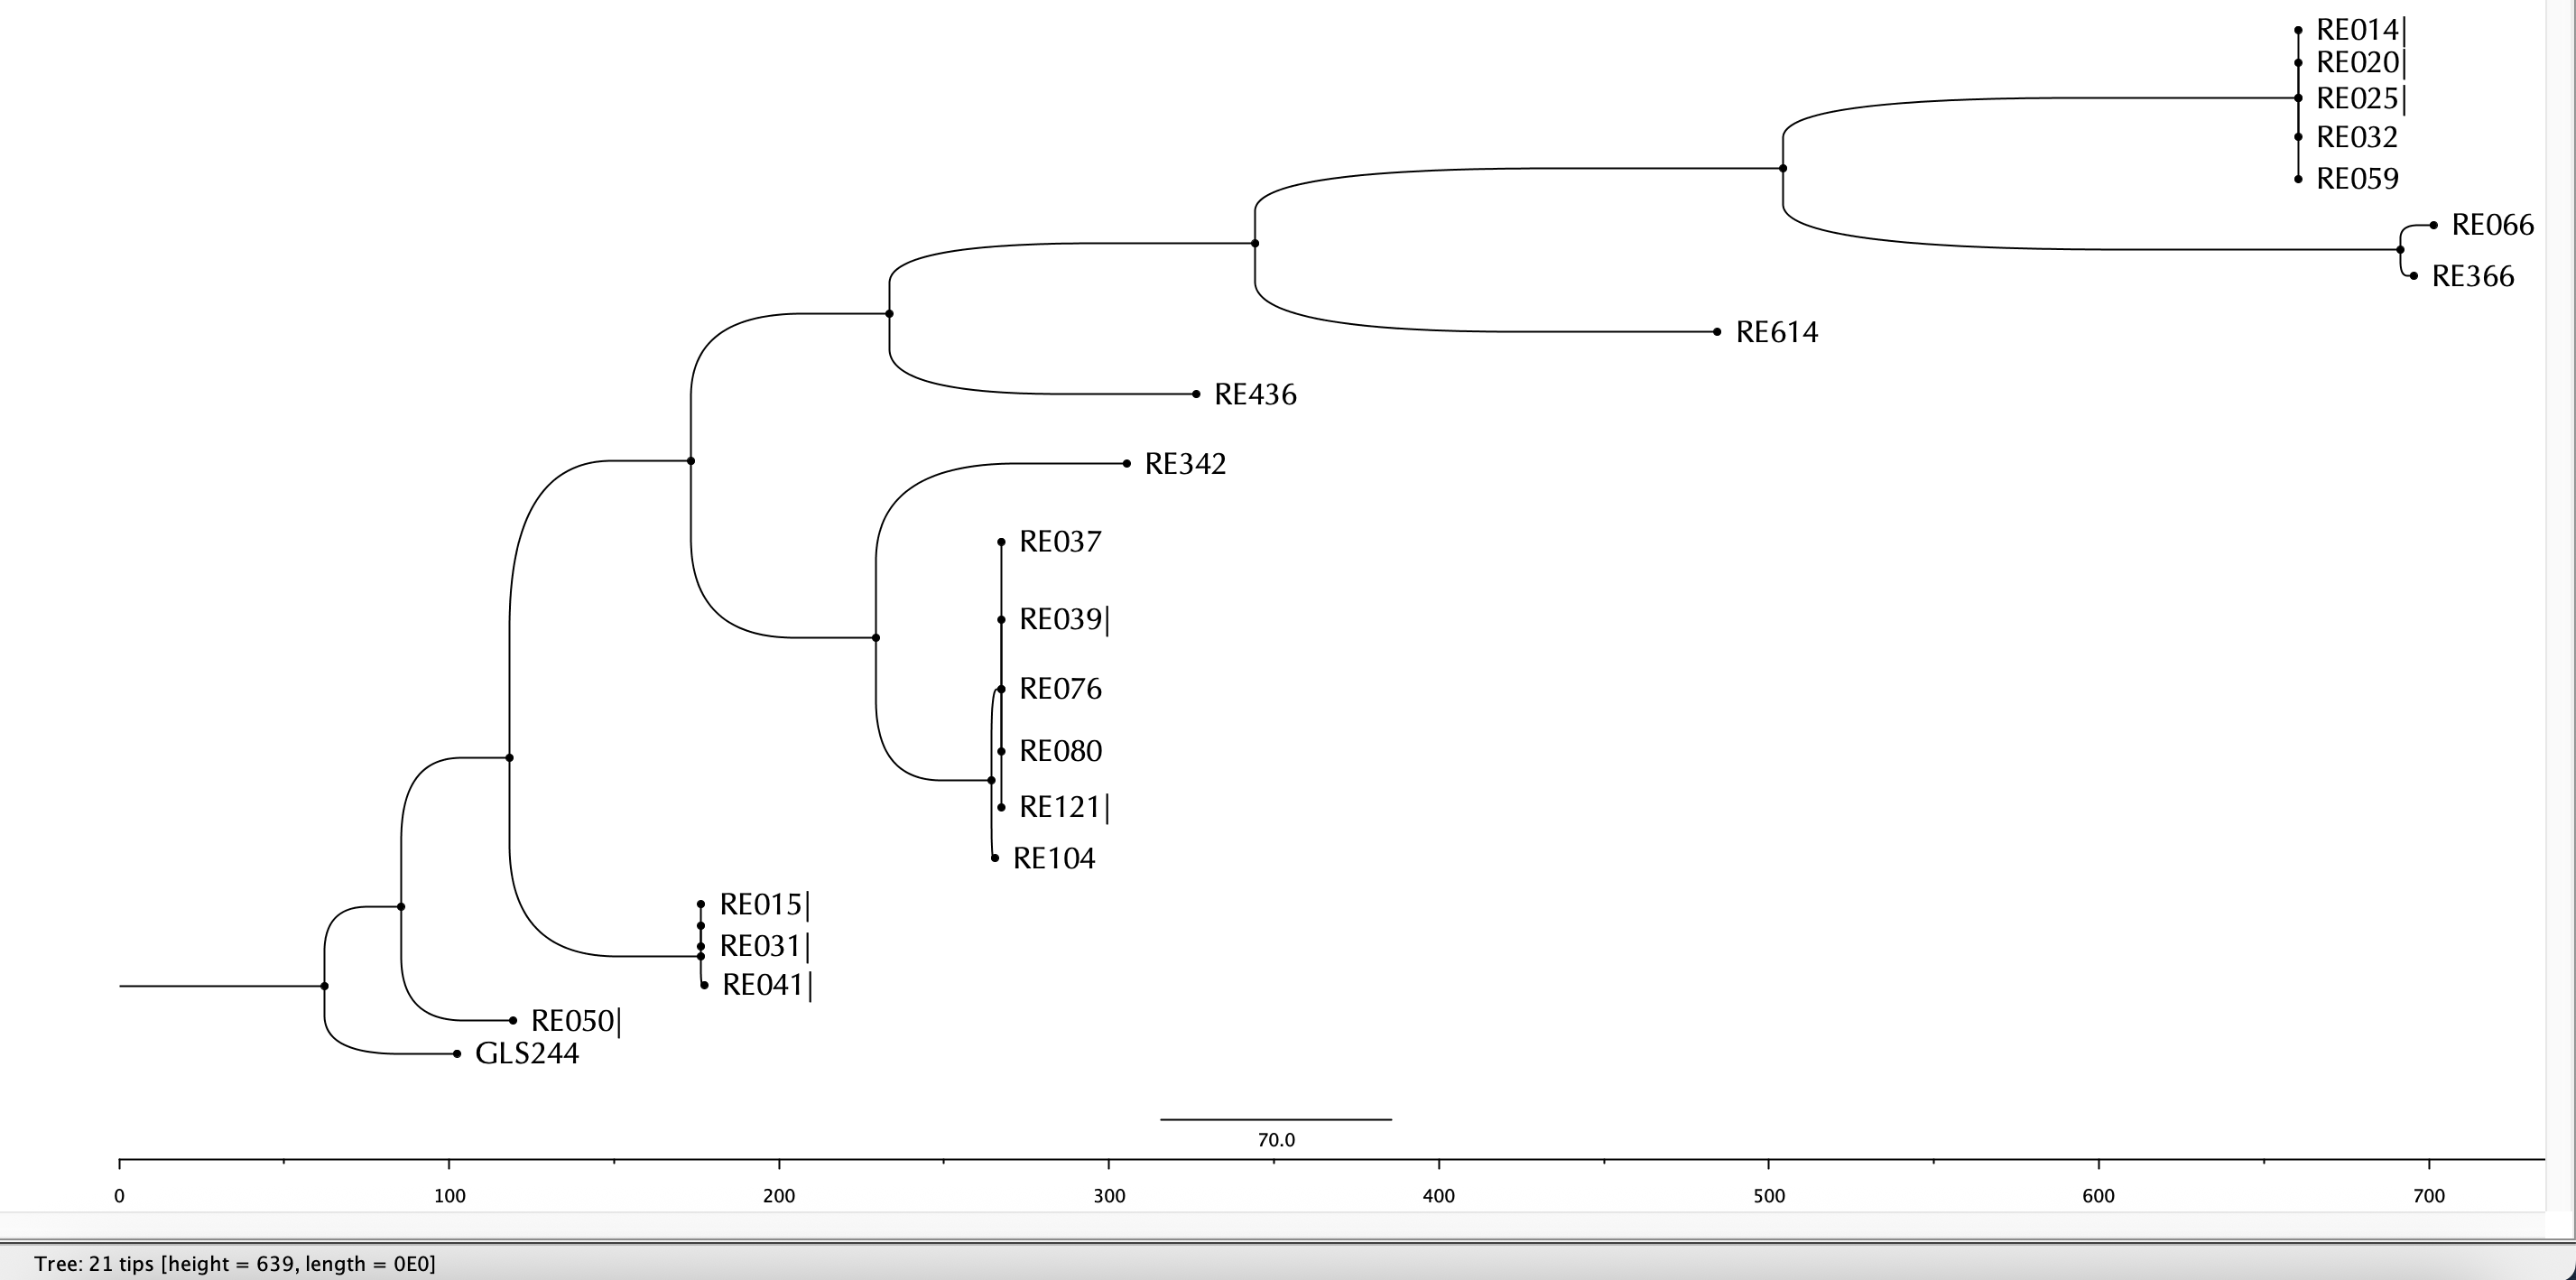
\includegraphics[width=1\linewidth]{Images/FigTree_Consensus_Tree} 

}

\caption{ Consensus Tree}\label{fig:unnamed-chunk-40}
\end{figure}

\newpage

\subsection{WebLogo}\label{weblogo}

To investigate patterns of sequence conservation and variability, a
sequence logo was generated using the aligned sequences as input. This
visualisation facilitated the identification of conserved motifs and
regions of high sequence variability. The sequence logo revealed that
the conservations was primarily limited to the N-terminal and C-
terminal regions while the central portion of the alignment exhibited
variation.

For clarity and relevance, only representative segments of the logo
corresponding to the highly conserved and highly variable regions are
presented herein, rather than displaying the full alignment.

These patterns support the interpretation that conserved regions may be
subject to purifying selection and thus potentially involved in
essential structural or functional roles. In contrast, variable regions
may reflect positive selection pressures, possibly contributing to
immune evasion mechanisms in the host-pathogen interaction.

\begin{figure}

{\centering 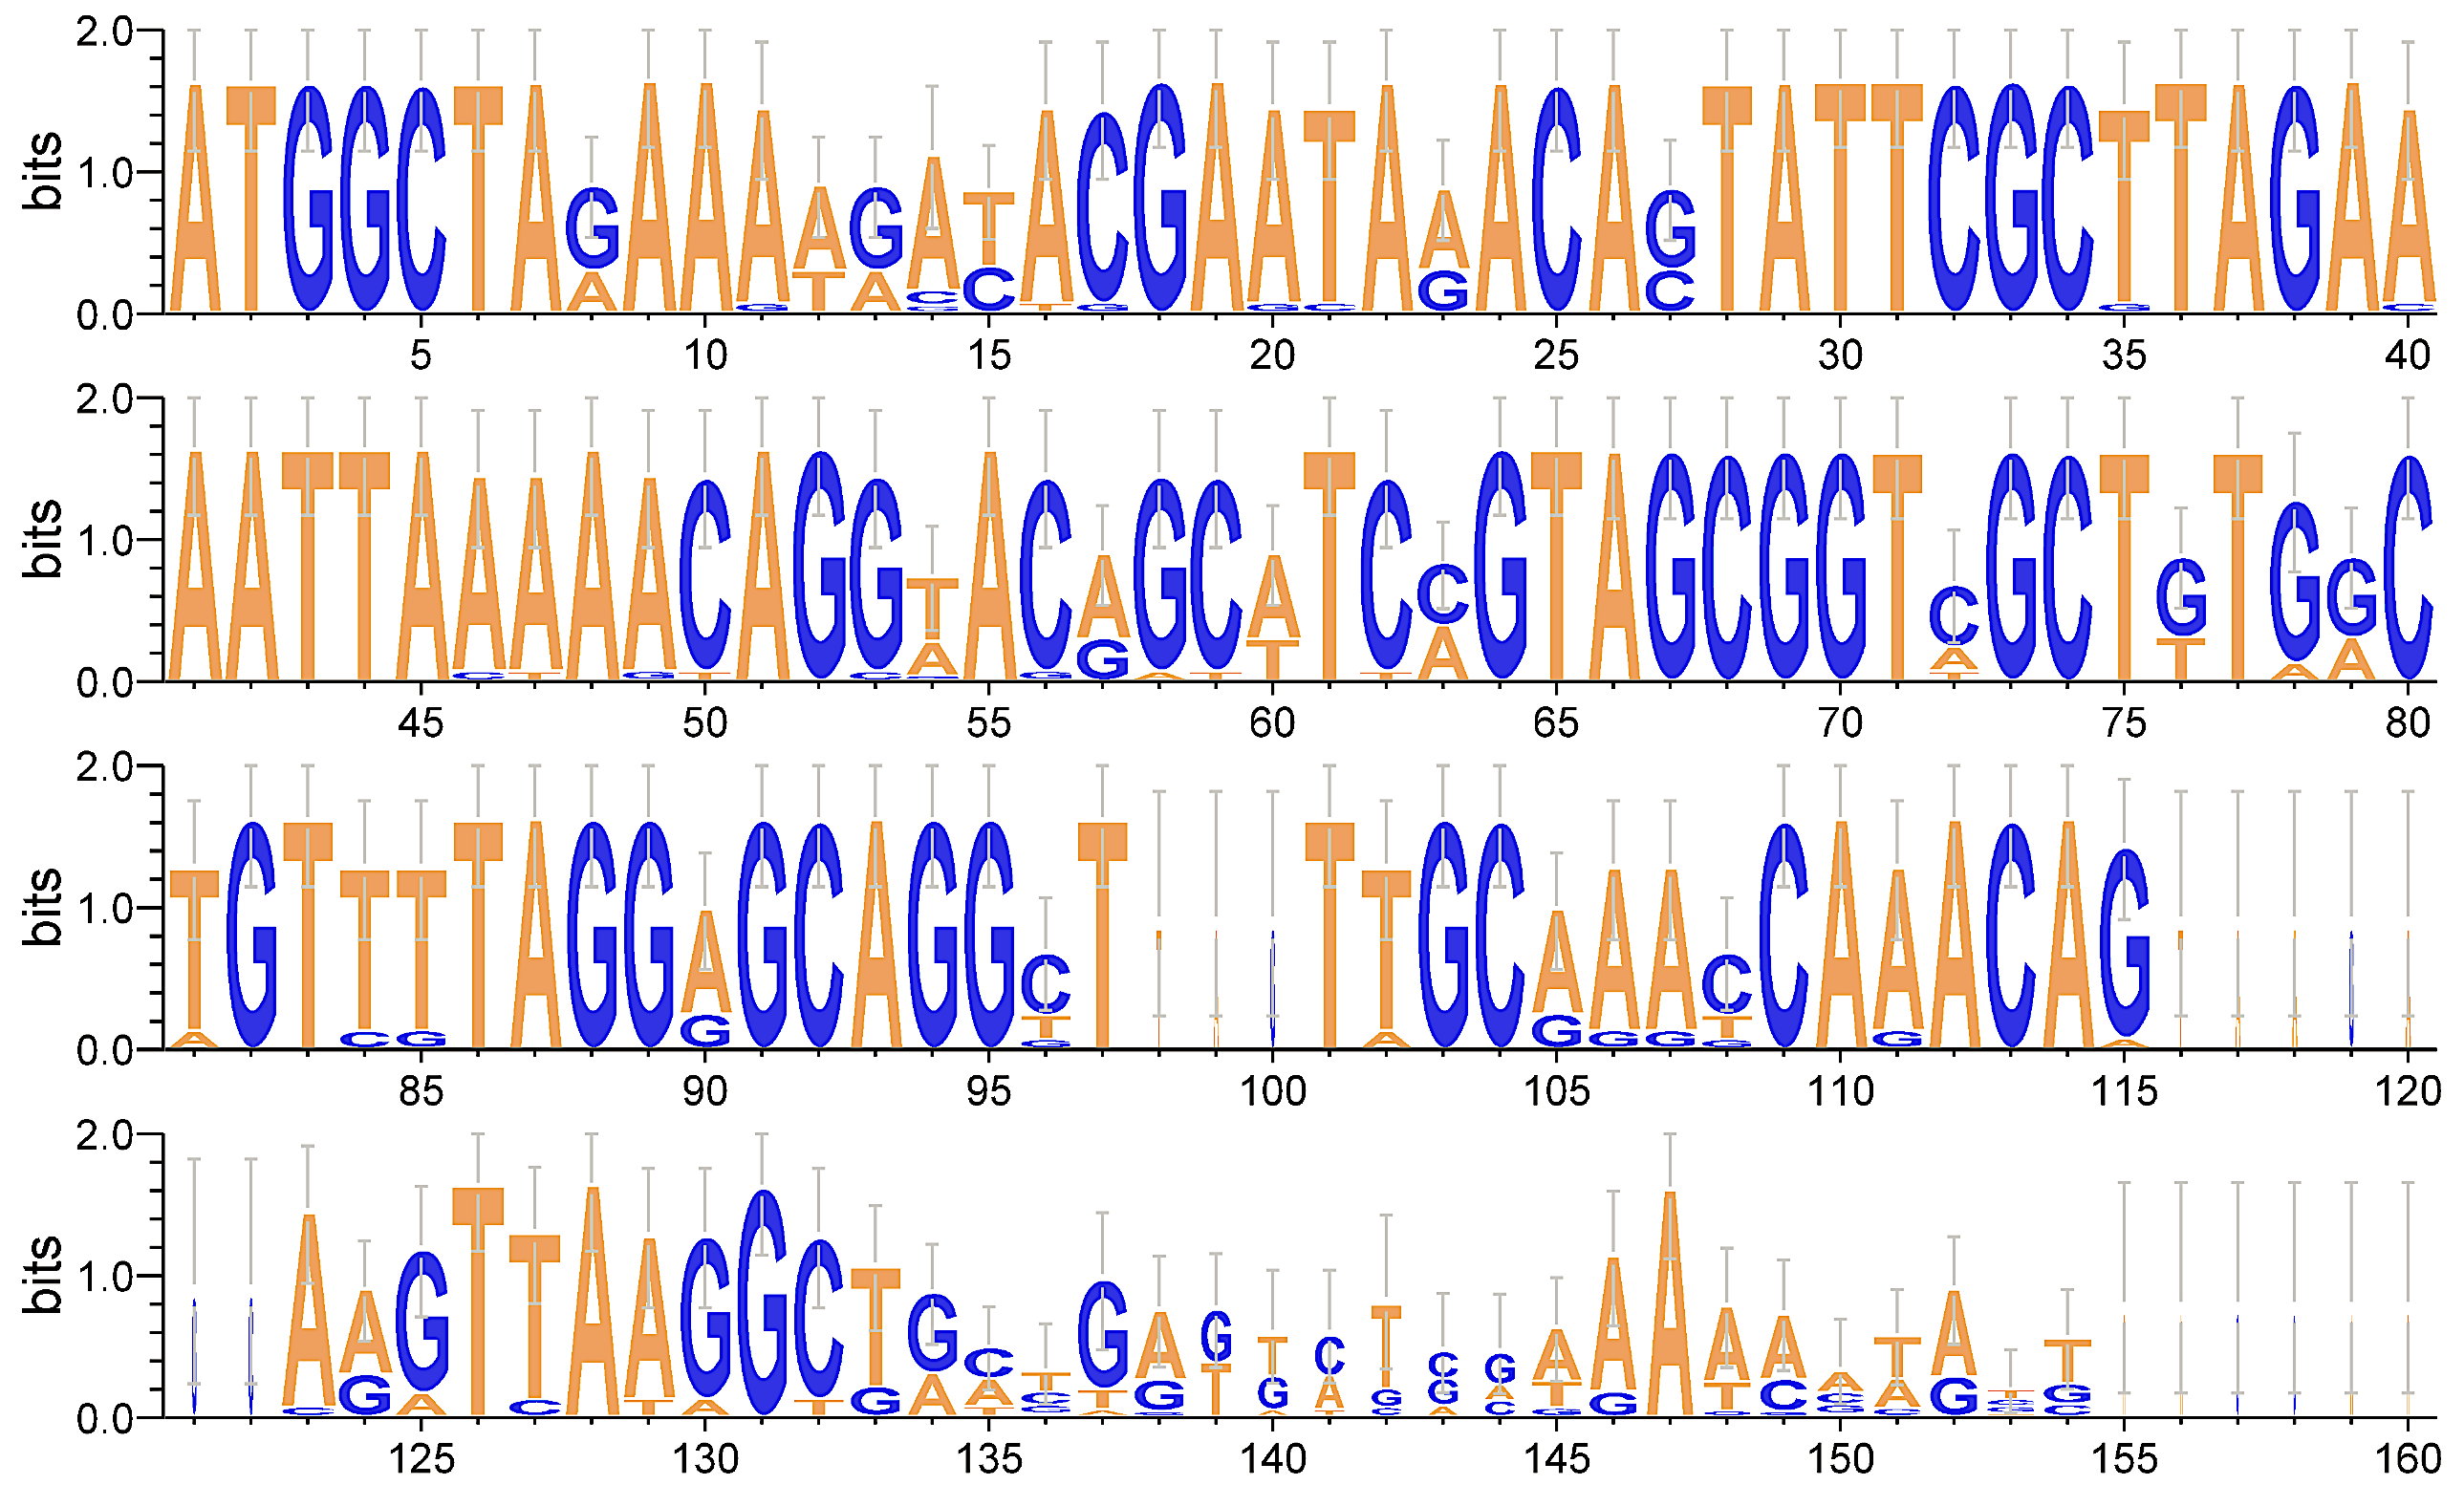
\includegraphics[width=0.6\linewidth]{Images/WebLogo1} 

}

\caption{Sequence Logo 1}\label{fig:unnamed-chunk-41}
\end{figure}

\begin{figure}

{\centering 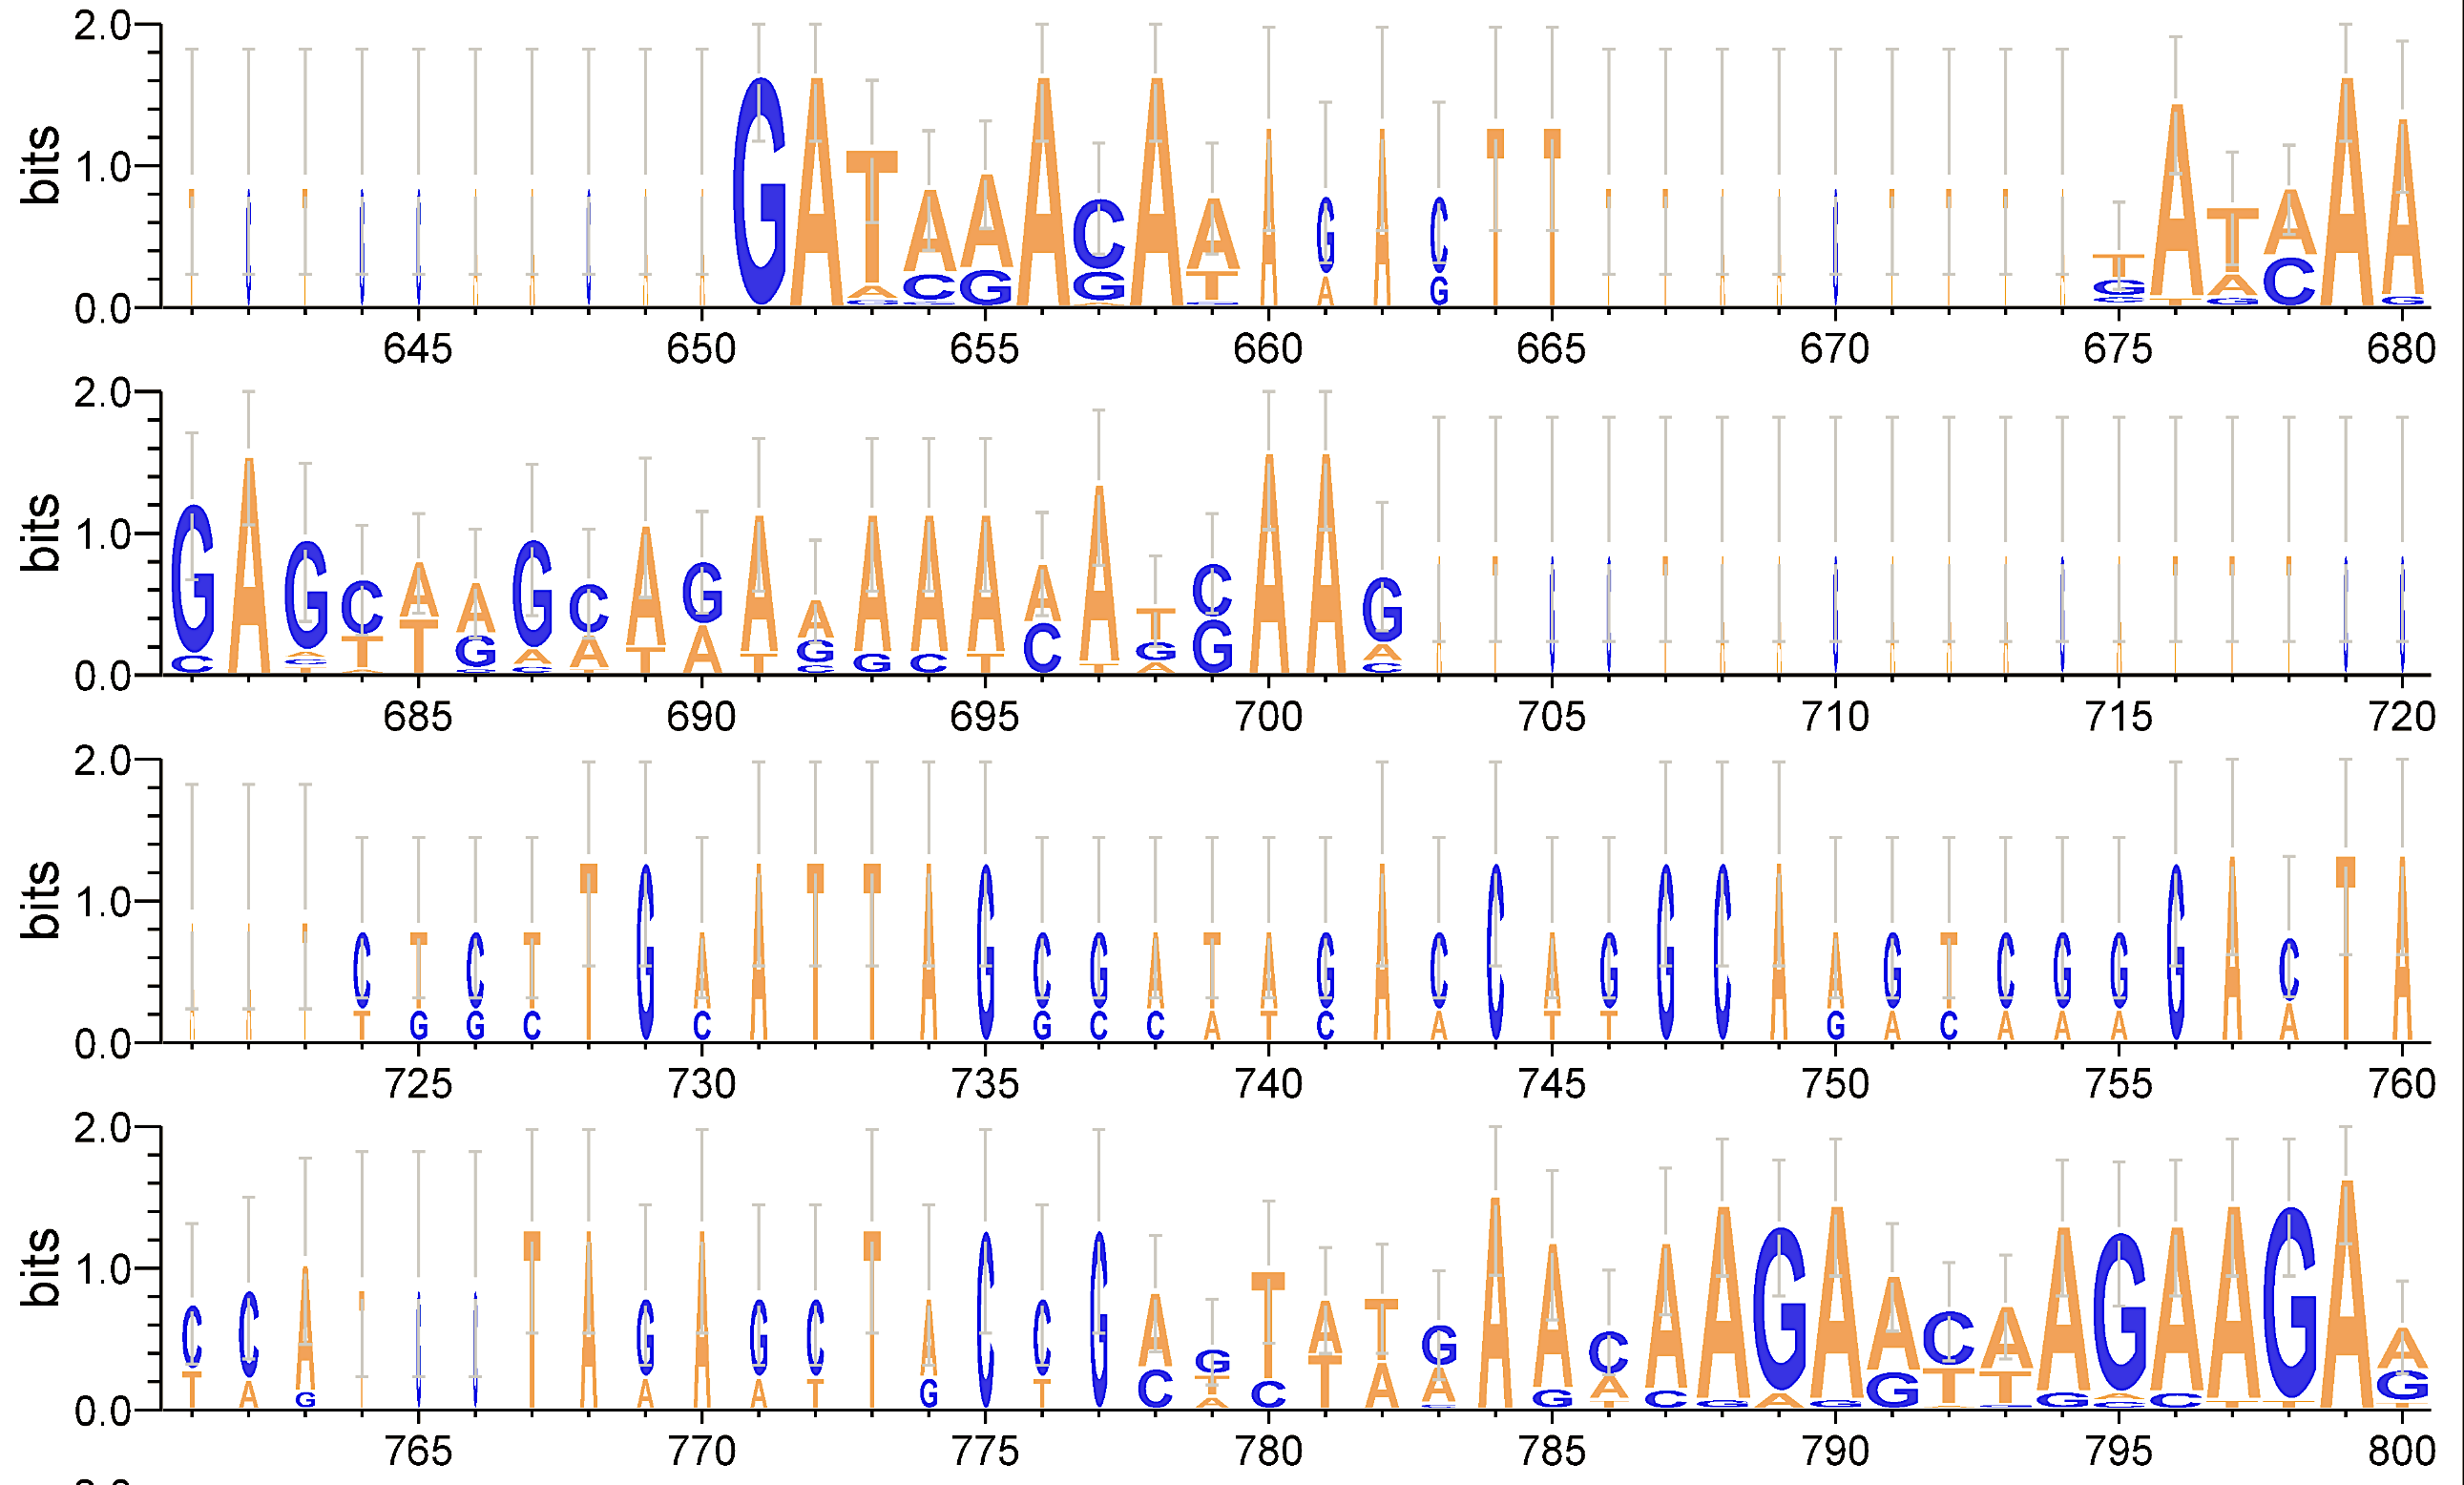
\includegraphics[width=0.6\linewidth]{Images/WebLogo2} 

}

\caption{ Sequence Logo 2}\label{fig:unnamed-chunk-42}
\end{figure}

\begin{figure}

{\centering 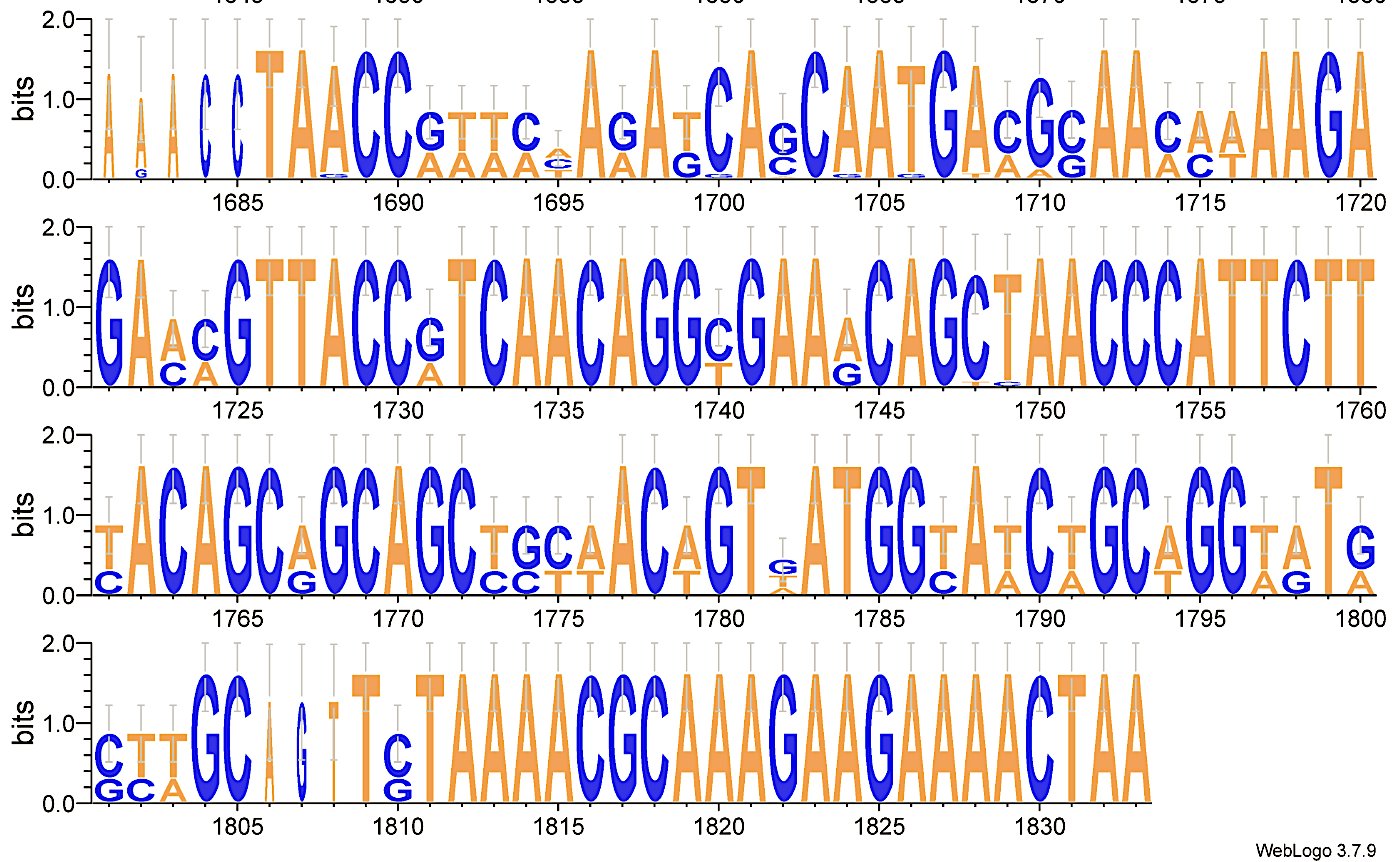
\includegraphics[width=0.6\linewidth]{Images/WebLogo3} 

}

\caption{ Sequence Logo 3}\label{fig:unnamed-chunk-43}
\end{figure}

\newpage

\subsection{AlphaFold three-dimensional protein structure
prediction}\label{alphafold-three-dimensional-protein-structure-prediction}

\begin{figure}

{\centering 
\includegraphics[width=1\linewidth]{Images/Alpha} 

}

\caption{AlphaFold}\label{fig:unnamed-chunk-44}
\end{figure}

Based on the amino acid sequence provided in the original FASTA file,
the corresponding M protein sequence was retrieved in FASTA format.

To predict the three-dimensional structure of the M protein, the amino
acid sequence was submitted to AlphaFold, which uses deep learning to
infer protein folding patterns.

A BLASTP search was performed against the protein structure database to
identify homologous structures. The search returned a 100\% identity
match with a known M protein sequence in UniProt (accession W0T1Y4).

The predicted structure was examined using PyMOL, a molecular
visualisation system. Screenshots of the structural model of the M
Protein are provided below\textsuperscript{32}.

The M protein is encoded by the emm28 gene from Streptococcus pyogenes,
has a UniProt ID of W0T1Y4, consists of 393 amino acids in length, and
is identified in the Protein Data Bank as AF-W0T1Y4-F1-v4.

\newpage

\begin{figure}

{\centering 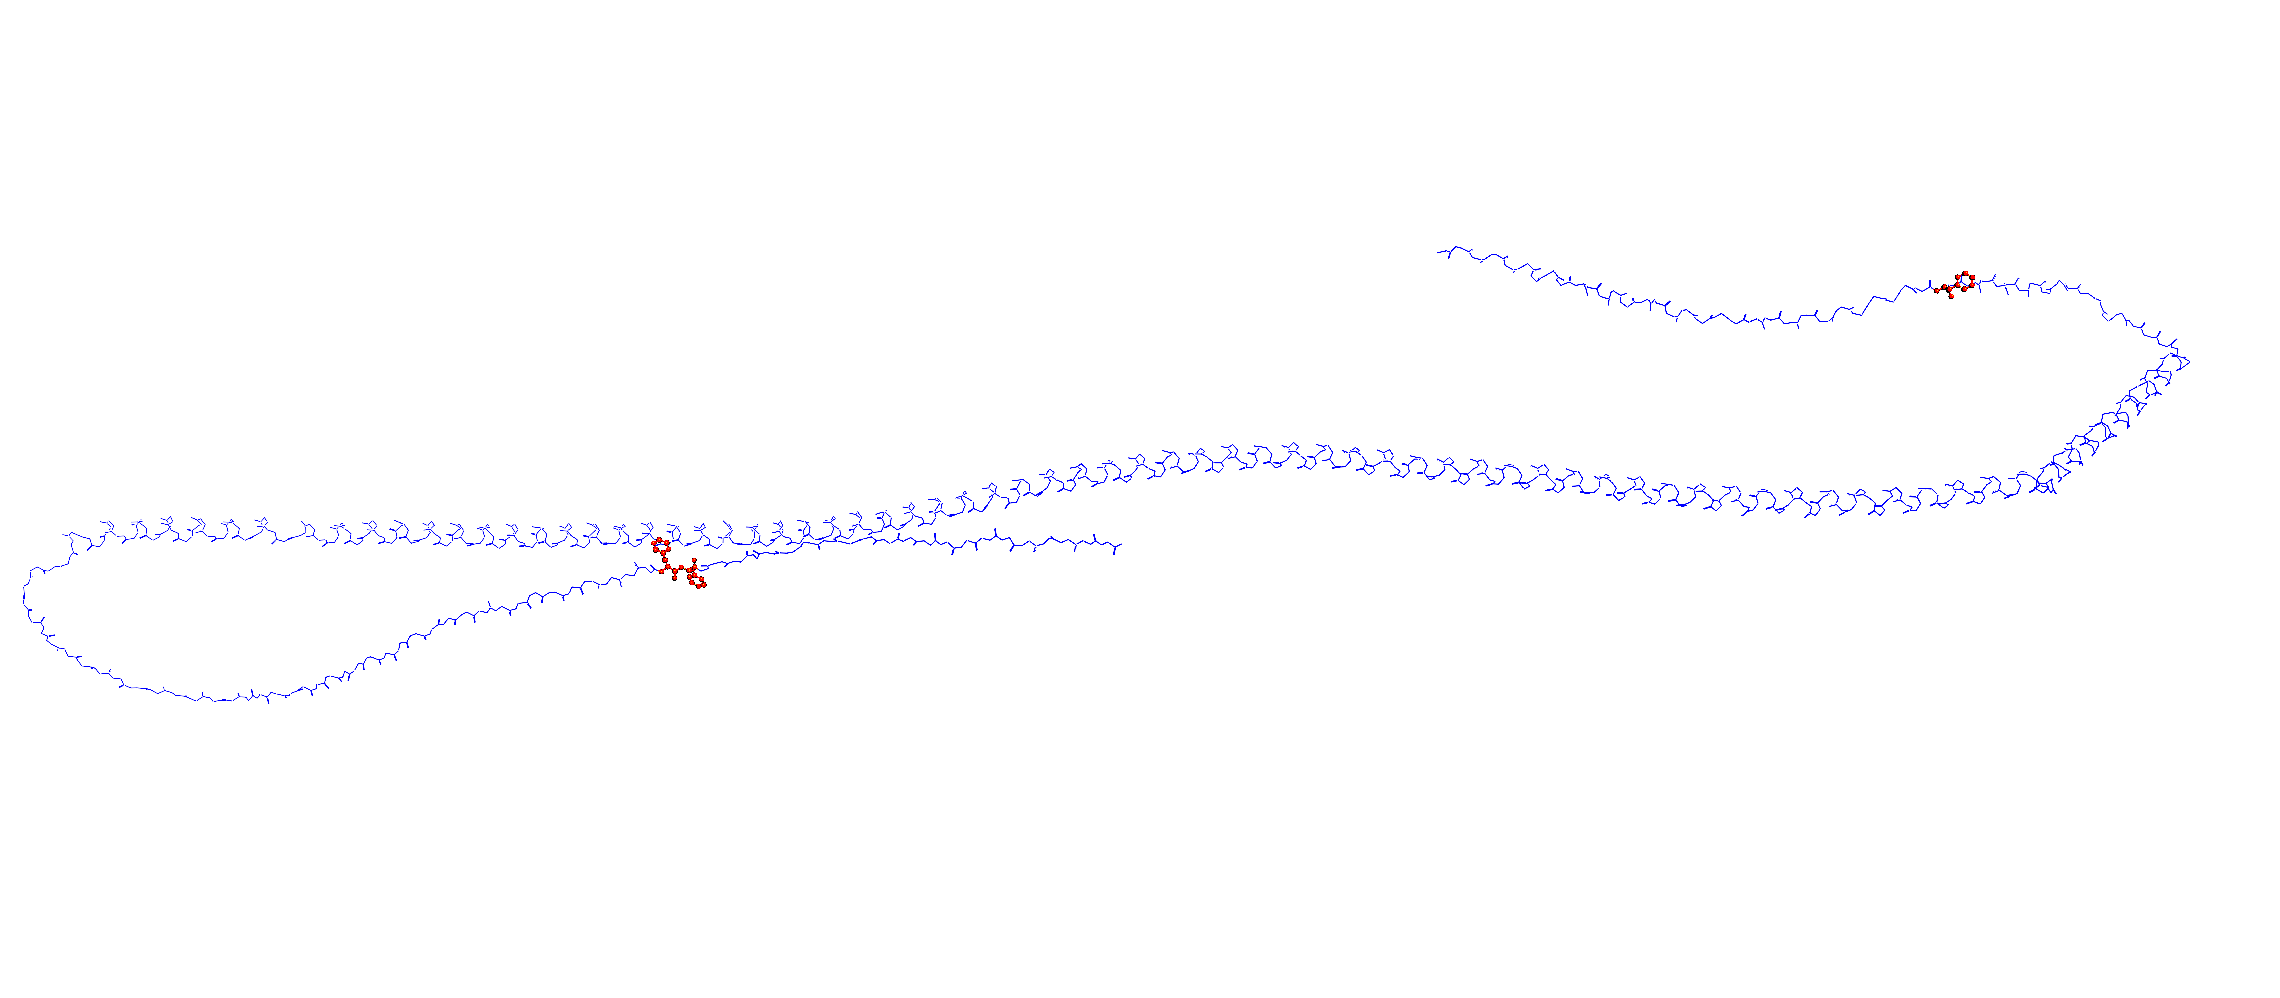
\includegraphics[width=1\linewidth]{Images/mprotein2} 

}

\caption{M Protein expressed from emm28 gene - Pymol}\label{fig:unnamed-chunk-46}
\end{figure}

\begin{figure}

{\centering 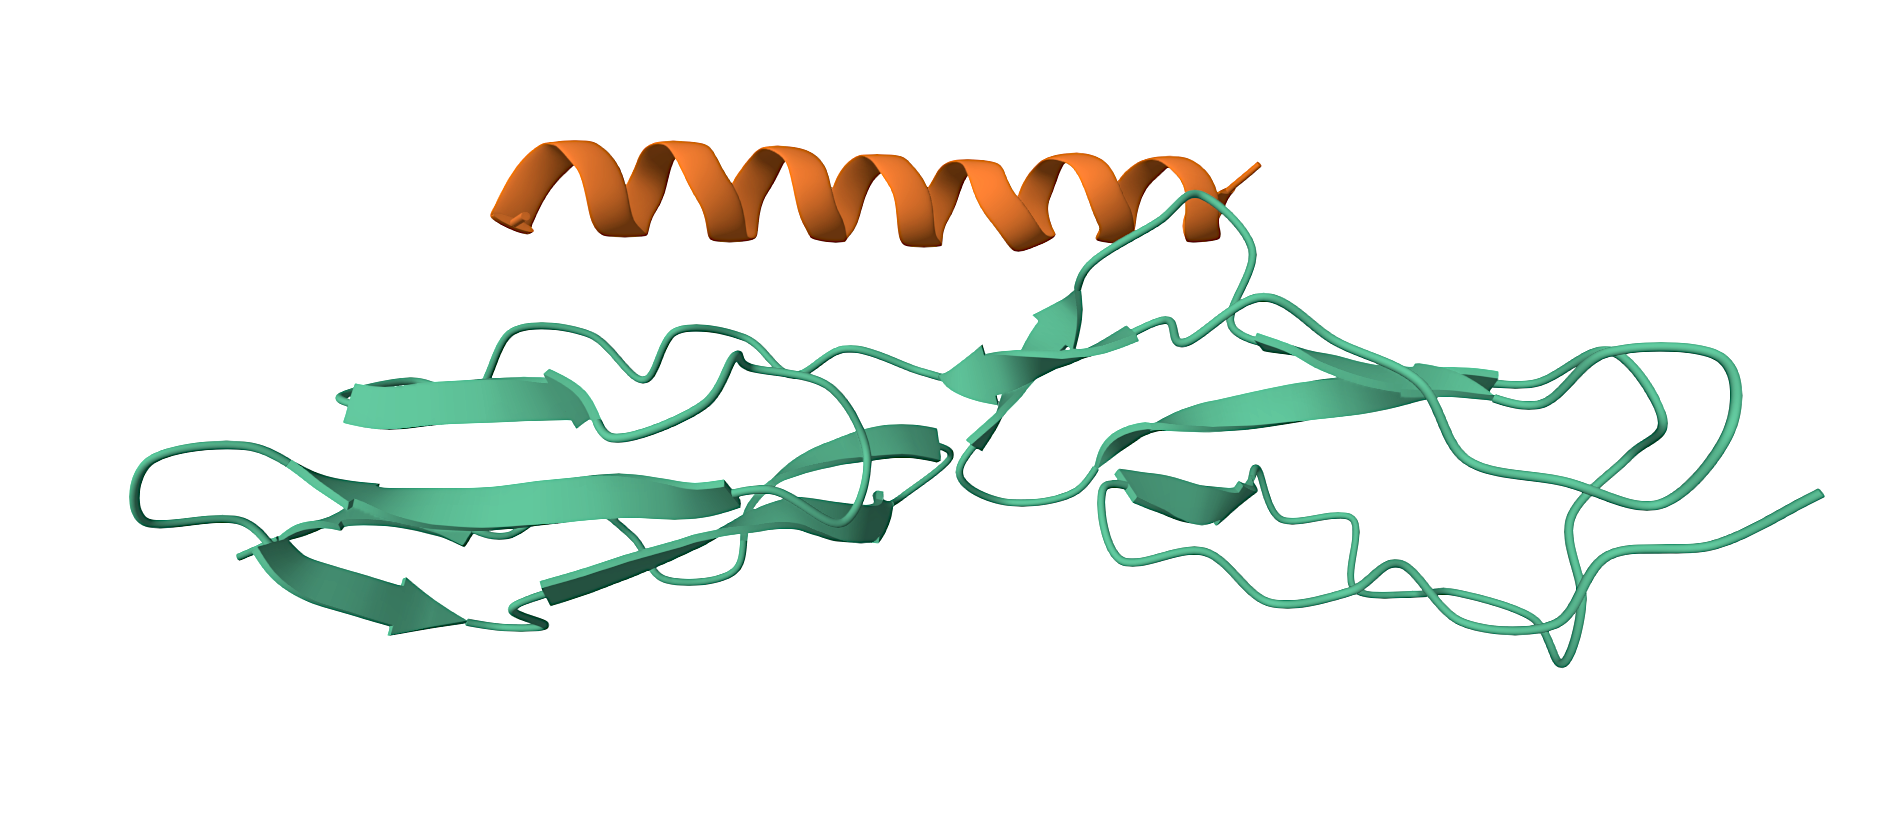
\includegraphics[width=1\linewidth]{Images/Uniprot_M_Protein} 

}

\caption{M Protein expressed from emm28 gene from UniProt}\label{fig:unnamed-chunk-47}
\end{figure}

\newpage

\section{CHAPTER V : CONCLUSION}\label{chapter-v-conclusion}

This bioinformatic investigation examined differential gene expression
profiles between melanoma and nevus skin samples, using analytical
approaches to reveal molecular signatures and pathways associated with
Melanoma. The thesis contains various visualisation methods and uses
computational tools to identify specific genes and characterise the
underlying biological processes governing the transition from benign to
malignant skin lesions.

The differential expression analysis revealed distinct molecular
signatures distinguishing melanoma from nevus samples. Volcano plot
visualisation demonstrated clear separation of significantly
up-regulated and down-regulated genes, with log₁₀ p-values plotted
against log₂ fold changes revealing robust statistical significance.
Among the most prominently unregulated genes in melanoma samples were
NTRK3, RASGRF1, SPP1, HEY1, GDF15, and BCL2A1, while genes including
KRT15, SERPINB5, LY6D, HOPX, SFN, CHL1, and FLG exhibited significant
down-regulation. These findings were corroborated by MA plot analysis,
which confirmed the magnitude and significance of expression changes.

Principal Component Analysis revealed intriguing clustering patterns,
with one melanoma sample demonstrating molecular similarity to nevus
samples, suggesting potential transitional states or heterogeneity
within the dataset. This observation was further supported by
correlation heatmap analysis, where melanoma sample GSM71709 clustered
with nevus samples GSM71680 and GSM71694, indicating shared expression
profiles that may represent intermediate stages of transformation. UMAP
dimensionality reduction analysis reinforced these findings, showing
that nevus sample GSM71680 clustered proximal to multiple melanoma
samples, implying potential early transformation characteristics or
biological similarity.

Gene Ontology enrichment analysis identified several key biological
processes significantly associated with the differentially expressed
genes. The analysis revealed enrichment of processes related to
epidermis development, regulation of nervous system development, neuron
projection development, and epithelial cell proliferation, while
keratinocyte differentiation pathways showed reduced enrichment. These
findings suggest that melanoma development involves dysregulation of
fundamental keratinocyte differentiation.

KEGG pathway analysis elucidated several crucial signalling cascades and
biological processes altered in melanoma progression. Significantly
enriched pathways included cornified envelope formation, PI3K-Akt
signalling, focal adhesion, proteoglycans in cancer, axon guidance, and
efferocytosis. Notably, genes associated with human papillomavirus
infection were also enriched, which may have clinical relevance given
the established relationship between HPV and various skin pathologies.

Gene Set Enrichment Analysis provided additional validation of the
differential expression patterns through examination of predefined gene
signatures. The analysis of the top 20 up-regulated genes in melanoma
demonstrated significant enrichment with a mean difference of 0.524 and
adjusted p-value of 4.53×10⁻¹⁴, confirming a distinct
melanoma-associated expression profile.

Tumour microenvironment analysis using the ESTIMATE algorithm provided
insights into the cellular composition of the samples. Melanoma samples
exhibited lower stromal scores, indicating reduced stromal cell
infiltration, while demonstrating higher immune scores suggestive of
increased immune cell presence. This pattern may reflect the
inflammatory response associated with malignant transformation or immune
surveillance mechanisms.

ESTIMATE scores, which integrate both stromal and immune components,
were marginally elevated in nevus samples. Tumour purity assessment
revealed high values (approximately 0.8) in both sample types.

The phylogenetic analysis revealed strain clustering based on emm gene
types, with emm1 and emm12 strains forming distinct evolutionary clades,
suggesting conservation of genetic features within specific emm
classifications. Sequence alignment and WebLogo analysis of the M
protein identified highly conserved regions at both N- and C-termini,
which likely play crucial roles in structural stability and functional
integrity. The identification of phenylalanine residues at terminal
positions is particularly noteworthy, as these aromatic, hydrophobic
amino acids are relatively uncommon and may contribute to important
structural or binding functions. The hydrophobic nature of phenylalanine
suggests potential roles in membrane anchoring, protein-protein
interactions, or tertiary structure stabilisation.

The presence of sulphur containing residues in the M protein , likely
cysteines, indicates the potential for disulphide bond formation, which
is known to confer mechanical stability and is particularly relevant in
skin and hair-associated proteins. The conservation of phenylalanine
residues across multiple protein homologs implies strong evolutionary
pressure for their maintenance, suggesting critical functional roles in
protein folding, membrane association, or binding specificity. PyMOL
visualisation confirmed the distinct positioning of these residues,
potentially highlighting important binding or anchoring sites within the
protein structure.

The molecular patterns observed in this study provide valuable insights
into the complex biological processes underlying melanoma development
and progression. However, several limitations must be acknowledged. The
dataset contained only seven normal skin samples, which limited the
statistical power for comprehensive comparisons with both nevus and
melanoma tissues. Future investigations should incorporate larger,
well-annotated cohorts including adequate numbers of normal skin samples
to better delineate the molecular changes occurring during early-stage
melanoma development. In conclusion, this comprehensive bioinformatic
analysis has successfully identified distinct molecular signatures
differentiating melanoma from nevus samples, revealed key pathways, and
characterised the tumour microenvironment composition.

\newpage

\section{Appendices}\label{appendices}

\subsubsection{Pymol Script to display M protein
structure}\label{pymol-script-to-display-m-protein-structure}

\begin{Shaded}
\begin{Highlighting}[]
\CommentTok{\# PyMOL script to display structure}

\CommentTok{\# Hide everything first}
\ExtensionTok{hide}\NormalTok{ everything}

\CommentTok{\# Show the carbon backbone as thin wire}
\ExtensionTok{show}\NormalTok{ wire, name CA}
\BuiltInTok{set}\NormalTok{ stick\_radius, 0.1, name CA}

\CommentTok{\# Alternatively, you can show the entire backbone as thin wire:}
\ExtensionTok{show}\NormalTok{ wire, backbone}
\BuiltInTok{set}\NormalTok{ stick\_radius, 0.1, backbone}

\CommentTok{\# Select phenylalanine residues}
\ControlFlowTok{select}\NormalTok{ phe\_residues}\ExtensionTok{,}\NormalTok{ resn PHE}

\CommentTok{\# Show phenylalanine residues as ball and stick}
\ExtensionTok{show}\NormalTok{ sticks, phe\_residues}
\ExtensionTok{show}\NormalTok{ spheres, phe\_residues}

\CommentTok{\# Color phenylalanine residues orange}
\ExtensionTok{color}\NormalTok{ orange, phe\_residues}

\CommentTok{\# Turn on valence display for phenylalanine residues}
\BuiltInTok{set}\NormalTok{ valence, on, phe\_residues}

\CommentTok{\# Optional: Adjust sphere and stick sizes for better visualization}
\BuiltInTok{set}\NormalTok{ sphere\_scale, 0.3, phe\_residues}
\BuiltInTok{set}\NormalTok{ stick\_radius, 0.15, phe\_residues}
\end{Highlighting}
\end{Shaded}

\newpage

Table: (Summary of MUSCLE Alignment Log for emm Genes Isolated from
Streptococcus pyogenes)

MUSCLE v3.8.1551 by Robert C. Edgar \textbar{}
\url{http://www.drive5.com/muscle}\textsuperscript{33}

\begin{longtable}[]{@{}lllll@{}}
\toprule\noalign{}
Time & Memory & Iteration & Progress & Step \\
\midrule\noalign{}
\endhead
\bottomrule\noalign{}
\endlastfoot
00:00:00 & 1 MB(0\%) & 1 & 100.00\% & K-mer dist pass 1 \\
00:00:00 & 1 MB(0\%) & 1 & 100.00\% & K-mer dist pass 2 \\
00:00:00 & 22 MB(0\%) & 1 & 100.00\% & Align node \\
00:00:00 & 22 MB(0\%) & 1 & 100.00\% & Root alignment \\
00:00:00 & 24 MB(0\%) & 2 & 100.00\% & Refine tree \\
00:00:00 & 24 MB(0\%) & 2 & 100.00\% & Root alignment \\
00:00:00 & 24 MB(0\%) & 2 & 100.00\% & Root alignment \\
00:00:01 & 24 MB(0\%) & 3 & 100.00\% & Refine biparts \\
00:00:03 & 24 MB(0\%) & 4 & 100.00\% & Refine biparts \\
00:00:03 & 24 MB(0\%) & 5 & 100.00\% & Refine biparts \\
00:00:03 & 24 MB(0\%) & 5 & 100.00\% & Refine biparts \\
\end{longtable}

PAUP Tree statistics

\begin{longtable}[]{@{}ll@{}}
\caption{( Tree Statistics from the Consensus Tree)}\tabularnewline
\toprule\noalign{}
Statistic & Value \\
\midrule\noalign{}
\endfirsthead
\toprule\noalign{}
Statistic & Value \\
\midrule\noalign{}
\endhead
\bottomrule\noalign{}
\endlastfoot
Tree length & 1336 \\
Consistency index (CI) & 0.8278 \\
Homoplasy index (HI) & 0.1722 \\
CI excluding uninformative characters & 0.7941 \\
HI excluding uninformative characters & 0.2059 \\
Retention index (RI) & 0.9095 \\
Rescaled consistency index (RC) & 0.7529 \\
\end{longtable}

\newpage

\section*{References}\label{references}
\addcontentsline{toc}{section}{References}

\phantomsection\label{refs}
\begin{CSLReferences}{0}{1}
\bibitem[\citeproctext]{ref-openai2023chatgpt}
\CSLLeftMargin{1. }%
\CSLRightInline{OpenAI, {``\emph{ChatGPT: Language model by OpenAI},''}
2023, accessed.}

\bibitem[\citeproctext]{ref-zoterobib2025}
\CSLLeftMargin{2. }%
\CSLRightInline{{``\emph{{ZoteroBib: Fast, Free Bibliography Generator -
MLA, APA, Chicago, Harvard Citations}},''} 2025, URL:
\url{https://zbib.org/}, accessed 13 May 2025.}

\bibitem[\citeproctext]{ref-noauthor_integumentary_nodate}
\CSLLeftMargin{3. }%
\CSLRightInline{{``\emph{Integumentary system: What it is, function \&
organs},''} \emph{Cleveland Clinic}, URL:
\url{https://my.clevelandclinic.org/health/body/22827-integumentary-system},
accessed 11 June 2025.}

\bibitem[\citeproctext]{ref-healthline2018layers}
\CSLLeftMargin{4. }%
\CSLRightInline{Healthline Editorial Team, {``\emph{Layers of skin: How
many, diagram, model, anatomy, in order},''} 5 January 2018, URL:
\url{https://www.healthline.com/health/layers-of-skin}, accessed.}

\bibitem[\citeproctext]{ref-microsoft_designer}
\CSLLeftMargin{5. }%
\CSLRightInline{Corporation, M., {``\emph{Microsoft designer},''} 2025,
URL: \url{https://designer.microsoft.com/}, accessed.}

\bibitem[\citeproctext]{ref-smith2016epidermis}
\CSLLeftMargin{6. }%
\CSLRightInline{Smith, Y., {``\emph{What is the epidermis?}''} 2016,
URL:
\url{https://www.news-medical.net/health/What-is-the-Epidermis.aspx},
accessed.}

\bibitem[\citeproctext]{ref-caon2020examination}
\CSLLeftMargin{7. }%
\CSLRightInline{Caon, M., {``\emph{Examination questions and answers in
basic anatomy and physiology: 2900 multiple choice questions and 64
essay topics},''} 2020,
DOI:\href{https://doi.org/10.1007/978-3-030-47314-3}{10.1007/978-3-030-47314-3},
URL: \url{https://doi.org/10.1007/978-3-030-47314-3}, accessed.}

\bibitem[\citeproctext]{ref-koike2018toll}
\CSLLeftMargin{8. }%
\CSLRightInline{Koike, S., K. Yamasaki, T. Yamauchi, M. Inoue, R.
Shimada-Ohmori, K. Tsuchiyama and S. Aiba, {``\emph{Toll-like receptors
2 and 3 enhance melanogenesis and melanosome transport in human
melanocytes},''} \emph{Pigment Cell \& Melanoma Research}, 2018,
DOI:\href{https://doi.org/10.1111/pcmr.12703}{10.1111/pcmr.12703}, URL:
\url{https://doi.org/10.1111/pcmr.12703}, accessed.}

\bibitem[\citeproctext]{ref-genome2025fibroblast}
\CSLLeftMargin{9. }%
\CSLRightInline{National Human Genome Research Institute,
{``\emph{Fibroblast},''} 2025, accessed.}

\bibitem[\citeproctext]{ref-clevelandclinic2025collagen}
\CSLLeftMargin{10. }%
\CSLRightInline{Cleveland Clinic, {``\emph{Collagen: What it is, types,
function \& benefits},''} 2025, URL:
\url{https://my.clevelandclinic.org/health/articles/23089-collagen},
accessed.}

\bibitem[\citeproctext]{ref-moon2021invitro}
\CSLLeftMargin{11. }%
\CSLRightInline{Moon, S. and others, {``\emph{In vitro models mimicking
immune response in the skin},''} \emph{Yonsei Medical Journal}, 2021,
DOI:\href{https://doi.org/10.3349/ymj.2021.62.11.969}{10.3349/ymj.2021.62.11.969},
URL: \url{https://doi.org/10.3349/ymj.2021.62.11.969}, accessed.}

\bibitem[\citeproctext]{ref-sweatglands_mayo}
\CSLLeftMargin{12. }%
\CSLRightInline{Mayo Clinic, {``\emph{Sweat glands},''} 2025, URL:
\url{https://www.mayoclinic.org/diseases-conditions/hyperhidrosis/multimedia/sweat-glands/img-20007980},
accessed.}

\bibitem[\citeproctext]{ref-verywell2025hypodermis}
\CSLLeftMargin{13. }%
\CSLRightInline{Verywell Health, {``\emph{What the hypodermis layer of
the skin does},''} 2025, URL:
\url{https://www.verywellhealth.com/the-hypodermis-is-the-lowermost-layer-of-skin-2710144},
accessed.}

\bibitem[\citeproctext]{ref-proctor2023_fibrinogen}
\CSLLeftMargin{14. }%
\CSLRightInline{Proctor, E.-J., H. R. Frost and B. Mantri,
{``\emph{Fibrinogen-binding m-related proteins facilitate the
recruitment of plasminogen by \emph{streptococcus pyogenes}},''}
\emph{Frontiers in Microbiology}, 2023,
DOI:\href{https://doi.org/10.3389/fmicb.2023.1069789}{10.3389/fmicb.2023.1069789},
URL: \url{https://doi.org/10.3389/fmicb.2023.1069789}, accessed.}

\bibitem[\citeproctext]{ref-abusaiba2023_review}
\CSLLeftMargin{15. }%
\CSLRightInline{Abusaiba, T. H. H., A. A. Hussein and T. F. Almahbob,
{``\emph{A review of \emph{streptococcus pyogenes}: Public health risk
factors, prevention and control},''} \emph{Qeios}, 2023,
DOI:\href{https://doi.org/10.32388/bcsybu}{10.32388/bcsybu}, URL:
\url{https://doi.org/10.32388/bcsybu}, accessed.}

\bibitem[\citeproctext]{ref-nci_streptococcus_pyogenes}
\CSLLeftMargin{16. }%
\CSLRightInline{National Cancer Institute, {``\emph{Streptococcus
pyogenes},''} 2025, URL: \url{https://ncithesaurus.nci.nih.gov},
accessed.}

\bibitem[\citeproctext]{ref-boutin2024_genomic}
\CSLLeftMargin{17. }%
\CSLRightInline{Boutin, S., B. Arnold, A. S. Alabi, S. Bélard, N.
Toepfner and D. Nurjadi, {``\emph{Genomic epidemiology of
\emph{streptococcus pyogenes} from pharyngeal and skin swabs in
gabon},''} \emph{Microbiology Spectrum}, 2024,
DOI:\href{https://doi.org/10.1128/spectrum.04265-23}{10.1128/spectrum.04265-23},
URL: \url{https://doi.org/10.1128/spectrum.04265-23}, accessed.}

\bibitem[\citeproctext]{ref-sinha2025nrp1}
\CSLLeftMargin{18. }%
\CSLRightInline{Sinha, A., A. Pouliot, F. Rizzolio and et al.,
{``\emph{Neuregulin-1 modulates melanoma invasiveness and therapeutic
response via ErbB signaling},''} \emph{Scientific Reports}, 2025,
DOI:\href{https://doi.org/10.1038/s41598-025-90917-0}{10.1038/s41598-025-90917-0},
URL: \url{https://www.nature.com/articles/s41598-025-90917-0},
accessed.}

\bibitem[\citeproctext]{ref-tao2024melanoma}
\CSLLeftMargin{19. }%
\CSLRightInline{Tao, R. E., J. N. Pixley, C. Ahn and S. R. Feldman,
{``\emph{Chapter 10: Melanoma biomarkers},''} \emph{Biomarkers in
dermatology}, 2024,
DOI:\href{https://doi.org/10.1007/978-3-031-66513-4_10}{10.1007/978-3-031-66513-4\_10},
URL: \url{https://doi.org/10.1007/978-3-031-66513-4_10}, accessed.}

\bibitem[\citeproctext]{ref-li2025integrating}
\CSLLeftMargin{20. }%
\CSLRightInline{Li, Q. and H. Li, {``\emph{Integrating bioinformatics
and machine learning to identify AhR-related gene signatures for
prognosis and tumor microenvironment modulation in melanoma},''}
\emph{Frontiers in Immunology}, 2025,
DOI:\href{https://doi.org/10.3389/fimmu.2024.1519345}{10.3389/fimmu.2024.1519345},
URL: \url{https://doi.org/10.3389/fimmu.2024.1519345}, accessed.}

\bibitem[\citeproctext]{ref-liu2022gene}
\CSLLeftMargin{21. }%
\CSLRightInline{Liu, M. and Y. Xu, {``\emph{Gene identification and
potential drug therapy for drug-resistant melanoma with bioinformatics
and deep learning technology},''} \emph{Disease Markers}, 2022,
DOI:\href{https://doi.org/10.1155/2022/2461055}{10.1155/2022/2461055},
URL: \url{https://doi.org/10.1155/2022/2461055}, accessed.}

\bibitem[\citeproctext]{ref-mayo2025melanoma}
\CSLLeftMargin{22. }%
\CSLRightInline{Mayo Clinic, {``\emph{Melanoma - symptoms and
causes},''} 2025, accessed.}

\bibitem[\citeproctext]{ref-jayaraj2024bioinformatics}
\CSLLeftMargin{23. }%
\CSLRightInline{Jayaraj, P., T. Bhimwal, K. Kaur, K. Gupta, S. Taluja
and A. Priyadarshani, {``\emph{A bioinformatics approach to reveal
common genes and molecular pathways shared by cutaneous melanoma and
uveal melanoma},''} \emph{Egyptian Journal of Medical Human Genetics},
2024,
DOI:\href{https://doi.org/10.1186/s43042-024-00526-1}{10.1186/s43042-024-00526-1},
URL: \url{https://doi.org/10.1186/s43042-024-00526-1}, accessed.}

\bibitem[\citeproctext]{ref-xie2025centromere}
\CSLLeftMargin{24. }%
\CSLRightInline{Xie, L., K. Shen, C. Wei, J. Xuan, J. Huang, Z. Gao, M.
Ren, L. Wang, Y. Zhu, S. Zheng and et al., {``\emph{Centromere protein f
is a potential prognostic biomarker and target for cutaneous
melanoma},''} \emph{Biomedicines}, 2025,
DOI:\href{https://doi.org/10.3390/biomedicines13040792}{10.3390/biomedicines13040792},
URL: \url{https://doi.org/10.3390/biomedicines13040792}, accessed.}

\bibitem[\citeproctext]{ref-tsetsos2025}
\CSLLeftMargin{25. }%
\CSLRightInline{Aikaterini Tsentemeidou, P. E., {``\emph{Melanoma ,
41},''} \emph{Otolaryngology study guide}, 2025,
DOI:\href{https://doi.org/10.1007/978-3-031-77374-7_41}{10.1007/978-3-031-77374-7\_41},
URL: \url{https://doi.org/10.1007/978-3-031-77374-7_41}, accessed.}

\bibitem[\citeproctext]{ref-xie2022identification}
\CSLLeftMargin{26. }%
\CSLRightInline{Xie, R., B. Li, L. Jia and Y. Li,
{``\emph{Identification of core genes and pathways in melanoma
metastasis via bioinformatics analysis},''} \emph{International Journal
of Molecular Sciences}, 2022,
DOI:\href{https://doi.org/10.3390/ijms23020794}{10.3390/ijms23020794},
URL: \url{https://doi.org/10.3390/ijms23020794}, accessed.}

\bibitem[\citeproctext]{ref-genbank_AB548438}
\CSLLeftMargin{27. }%
\CSLRightInline{Murayama, S. Y., M. Yoshino and K. Ubukata,
{``\emph{Streptococcus pyogenes emm28 gene for m protein, complete cds,
strain: RE015},''} 2014, URL:
\url{https://www.ncbi.nlm.nih.gov/nuccore/AB548438.1}, accessed.}

\bibitem[\citeproctext]{ref-larsson_aliview_2014}
\CSLLeftMargin{28. }%
\CSLRightInline{Larsson, A., {``\emph{{AliView}: A fast and lightweight
alignment viewer and editor for large datasets},''}
\emph{Bioinformatics}, 2014,
DOI:\href{https://doi.org/10.1093/bioinformatics/btu531}{10.1093/bioinformatics/btu531},
URL: \url{https://github.com/AliView/AliView}, accessed.}

\bibitem[\citeproctext]{ref-pedersen_seqconverter_2023}
\CSLLeftMargin{29. }%
\CSLRightInline{Pedersen, A. G., {``\emph{{seqconverter}: A command-line
tool for reading, writing, analyzing, and manipulating sequence
files},''} 2023,
DOI:\href{https://doi.org/10.5281/zenodo.10411474}{10.5281/zenodo.10411474},
URL: \url{https://github.com/agormp/seqconverter}, accessed.}

\bibitem[\citeproctext]{ref-swofford_paup_2003}
\CSLLeftMargin{30. }%
\CSLRightInline{Swofford, D. L., {``\emph{{PAUP\*}: Phylogenetic
analysis using parsimony (*and other methods)},''} 2003, accessed.}

\bibitem[\citeproctext]{ref-rambaut_figtree_2009}
\CSLLeftMargin{31. }%
\CSLRightInline{Rambaut, A., {``\emph{{FigTree} (version 1.4.x)},''}
2009, accessed.}

\bibitem[\citeproctext]{ref-uniprot_W0T1Y4}
\CSLLeftMargin{32. }%
\CSLRightInline{The UniProt Consortium, {``\emph{UniProtKB - W0T1Y4},''}
2025, URL: \url{https://www.uniprot.org/uniprotkb/W0T1Y4}, accessed.}

\bibitem[\citeproctext]{ref-edgar_muscle_2004}
\CSLLeftMargin{33. }%
\CSLRightInline{Edgar, R. C., {``\emph{{MUSCLE}: Multiple sequence
alignment with high accuracy and high throughput},''} \emph{Nucleic
Acids Research}, March 2004,
DOI:\href{https://doi.org/10.1093/nar/gkh340}{10.1093/nar/gkh340}, URL:
\url{http://www.drive5.com/muscle/}, accessed.}

\end{CSLReferences}

\end{document}
